%%%%%%%%%%%%%%%%%%%%%%%%%%%%%%%%%%%%%%%%%%%
%THIS FILE CONTAINS ALL COMMON COMMANDS NEEDED FOR COMPILATION INTO BOTH PDF AND HTML.
%THE EXTENSION file src/macros.sty CONTAINS ONLY COMMANDS NEEDED EXCLUSIVELY FOR COMPILATION INTO PDF
%THE DIRECTORY src/hva/ CONTAINS ONLY COMMANDS NEEDED EXCLUSIVELY FOR COMPILATION INTO HTML, WITH THREE EXTENSION FILES, imakeidx.hva, macros.hva AND picins.hva.
% This English Manual version was adapted from the orignail grisbi-manuel.tex by Bob Anderson, January 2018
%%%%%%%%%%%%%%%%%%%%%%%%%%%%%%%%%%%%%%%%%%%

\ifx\pdfoutput\undefined
\documentclass[a4paper,12pt,oneside]{book}
\else
\documentclass[pdftex,a4paper,12pt,twoside]{book}
\fi

\usepackage{ifpdf}

\usepackage[T1]{fontenc}			% the font encoding

\usepackage[utf8]{inputenc}			% the present input encoding
% Bob Anderson disabled the next 2 lines to prevent translation to french language ot LaTeX entries
%\usepackage[frenchb]{babel}			% the language TODO: make this customizable ; frenchb in place of french
\usepackage[frenchb]{translator}	% for translating the Fixed Names

\usepackage{textcomp}				% for special characters like \textcurrency
%\usepackage{txfonts}
%\usepackage{ae}
%\usepackage{cmbright}
\usepackage{times}					% changed from txfonts

% Web addresses
\usepackage{url}
%%%%%%%%%%%%%%%%%%%%%%%%%%%%%%%%%%%%%%%%%%%%%%%%%%%%%%%%%%%%%%%
% Contents: The url chapter
% $Id: grisbi-manuel-urldef.tex, modified from previous file :
% $Id: grisbi-manuel-urldef.tex, v 0.8.8 2011/XX/XX Jean-Luc Duflot
% $Id: grisbi-manuel-urldef.tex, v 1.0 2014/02/12 Jean-Luc Duflot
%%%%%%%%%%%%%%%%%%%%%%%%%%%%%%%%%%%%%%%%%%%%%%%%%%%%%%%%%%%%%%%


\urldef{\urlBob}%
\url{http://www.scilutions.co.uk}

\urldef{\urlMetonym}%
\url{https://literarydevices.net/metonymy/}

\urldef{\urlGitDoc}%
\url{https://github.com/grisbi/grisbi-documentation}

\urldef{\urlGtrans}%
\url{https://translate.google.com/}

\urldef{\urlGtransShell}%
\url{https://github.com/soimort/translate-shell}

\urldef{\urlBobDoc}%
\url{https://github.com/doubledodge/grisbi-documentation}




%%%%%%%%%%%%%%%%%%%%%%%%%%%%%%%%%%%%%%%%%%%%%%%%%%%%%%%%%%%%%%%
% Contents: The url chapter
% $Id: grisbi-manuel-urldef.tex, modified from previous file :
% $Id: grisbi-manuel-urldef.tex, v 0.8.8 2011/XX/XX Jean-Luc Duflot
% $Id: grisbi-manuel-urldef.tex, v 1.0 2014/02/12 Jean-Luc Duflot
%%%%%%%%%%%%%%%%%%%%%%%%%%%%%%%%%%%%%%%%%%%%%%%%%%%%%%%%%%%%%%%


\urldef{\urlGrisbi}%
\url{http://www.grisbi.org}

\urldef{\urlGrisbiTelechargement}%
\url{http://www.grisbi.org/download.fr.html}

\urldef{\urlBugTracker}%
\url{http://www.grisbi.org/bugsreports/}

\urldef{\urlGrisbiWiki}%
\url{http://wiki.grisbi.org/doku.php}

\urldef{\urlTuxFamily}%
\url{http://www.tuxfamily.org}

\urldef{\urlTuxFamilyMantis}%
\url{http://bugs.grisbi.org}

\urldef{\urlSourceForge}%
\url{http://sourceforge.net}

\urldef{\urlSourceForgeDocumentation}%
\url{http://sourceforge.net/projects/grisbi/files/Documentation}

\urldef{\urlGitGrisbi}%
\url{http://sourceforge.net/projects/grisbi/}

\urldef{\urlLinuxGraphic}%
\url{http://www.linuxgraphic.org}

\urldef{\urlFramasoftLogiciels}%
\url{http://www.framasoft.net/rubrique2.html}

\urldef{\urlGrisbiWin}%
\url{http://sourceforge.net/projects/grisbi4win/}

\urldef{\urlCygWin}%
\url{http://www.cygwin.com}

\urldef{\urlCyGnome}%
\url{http://cygnome.sourceforge.net}

\urldef{\urlAssociationsGouv}%
\url{http://www.associations.gouv.fr/704-comment-compter.html}

\urldef{\urlPlanComptable}%
\url{http://www.plancomptable.com/index.htm}

\urldef{\urlPlanDeComptes}%
\url{http://www.plancomptable.com/titre-IV/titre-IV_chapitre-III_section-1.htm#431-1}

\urldef{\urlListeComptes}%
\url{http://www.plancomptable.com/titre-IV/liste_des_comptes_sa.htm}

\urldef{\urlMaisonAssociations}%
\url{http://www.loi1901.com/regle_comptable.php}

\urldef{\urlComptaOnLine}%
\url{http://www.compta-online.com/pcg}

\urldef{\urlWikipedia}%
\url{http://fr.wikipedia.org/wiki/Wikipédia:Accueil_principal}

\urldef{\urlAndrePascualEmail}%
\url{andre@linuxgraphic.org}% without the leading "mailto:" for the DVI version

\urldef{\urlDanielCartronEmail}%
\url{daniel@cartron.org}    % without the leading "mailto:" for the DVI version

\urldef{\urlCedricAugerEmail}%
\url{cedric@grisbi.org}     % without the leading "mailto:" for the DVI version

\urldef{\urlSebastienBlondeelEmail}%
\url{sbi@april.org}% without the leading "mailto:" for the DVI version

\urldef{\urlGeraldNielEmail}%
\url{gerald@grisbi.org}% without the leading "mailto:" for the DVI version

\urldef{\urlBenjaminDrieuEmail}%
\url{bdrieu@april.org}     % without the leading "mailto:" for the DVI version

\urldef{\urlDionysosEmail}%
\url{dionysos@grisbi.org}     % without the leading "mailto:" for the DVI version

\urldef{\urlJulietteEmail}%
\url{juliette@grisbi.org}     % without the leading "mailto:" for the DVI version

\urldef{\urlFrancoisTerrotEmail}%
\url{grisbi@terrot.net}     % without the leading "mailto:" for the DVI version

\urldef{\urlLoicBreillouxEmail}%
\url{lbreilloux@users.sourceforge.net}    % without the leading "mailto:" for the DVI version

\urldef{\urlPierreBiavaEmail}%
\url{pierre.biava@nerim.net}     % without the leading "mailto:" for the DVI version

\urldef{\urlDidierChevalierEmail}%
\url{didier.chevalier35@gmail.com}     % without the leading "mailto:" for the DVI version

\urldef{\urlWilliamOllivierEmail}%
\url{guneeyoufix@gmail.com}     % without the leading "mailto:" for the DVI version

\urldef{\urlMickaelRemarsEmail}%
\url{grisbi@remars.com}     % without the leading "mailto:" for the DVI version

\urldef{\urlJeanLucDuflotEmail}%
\url{jl.duflot@laposte.net}     % without the leading "mailto:" for the DVI version

\urldef{\urlAlainLetientEmail}%
\url{al1.letient@free.fr}     % without the leading "mailto:" for the DVI version

\urldef{\urlGuyLebegueEmail}%
\url{guy@guy-lebegue.fr}     % without the leading "mailto:" for the DVI version

\urldef{\urlMicheleBondilEmail}%
\url{ciboulette05@club-internet.fr}     % without the leading "mailto:" for the DVI version

\urldef{\urlListInfoEmail}%
\url{grisbi-info@lists.sourceforge.net}     % without the leading "mailto:" for the DVI version

\urldef{\urlListDevelEmail}%
\url{devel@listes.grisbi.org}     % without the leading "mailto:" for the DVI version

\urldef{\urlListDocEmail}%
\url{grisbi-doc-fr@lists.sourceforge.net}     % without the leading "mailto:" for the DVI version

\urldef{\urlListTraductionEmail}%
\url{traduction@grisbi.org}  % without the leading "mailto:" for the DVI version

\urldef{\urlListWebmestre}%
\url{grisbi-website@lists.sourceforge.net}     % without the leading "mailto:" for the DVI version

\urldef{\urlListBugsreport}%
\url{bugsreports@listes.grisbi.org}     % without the leading "mailto:" for the DVI version

\urldef{\urlListSF}%
\url{http://lists.sourceforge.net/lists/listinfo/}     % without the leading "mailto:" for the DVI version





% --------------------------------------------
% Load graphicx package with pdf if needed
% --------------------------------------------
\ifpdf
\usepackage[pdftex]{graphicx}
%% Commented out to avoid errors in html, and put in the macros.sty file for pdf
%\pdfcompresslevel=9
\else
\usepackage{graphicx}
\fi

% Graphics Extensions
\ifpdf
\DeclareGraphicsExtensions{.pdf,.png,.jpg}
\else
\DeclareGraphicsExtensions{.eps}
\fi

% For illustrations
%\usepackage{picins}			% for text around image 
\usepackage{caption}		% for good references in table of figures


\usepackage{fancyhdr}
%\pagestyle{fancyplain}
%\usepackage{tabularx}
\usepackage{hhline}
\usepackage{layout}					% TODO: Only if DE mode
% Some of the following may also need to be commented out if more French creeps in to the English version?
\usepackage[french]{varioref}		% références in french
\usepackage{lastpage}
\usepackage{longtable}
\usepackage[dvips]{color}			% for a colored title page
%\usepackage{vmargin}				% for changing the title page margins
\usepackage{thumbpdf}


% Latex loads macros.sty for pdf output and Hevea loads /hva/macros.hva for html output
\usepackage{macros}


\definecolor{jaunegrisbi}{rgb}{1,1,.6}
\definecolor{bleugrisbi}{rgb}{.1,.1,.4}
\definecolor{vertgrisbi}{rgb}{0,.6,.4}
\definecolor{ocregrisbi}{rgb}{1,.7,0}


% Virtualization of fonts
\newcommand{\lang}[1]{\emph{#1}}
\newcommand{\familyname}[1]{\textsc{#1}}
\newcommand{\menu}[1]{\textsl{#1}}
\newcommand{\strong}[1]{\textsc{\textbf{#1}}}
\newcommand{\key}[1]{\texttt{<#1>}}
\newcommand{\cmd}[1]{\texttt{#1}}
\newcommand{\file}[1]{\textbf{#1}}
\newcommand{\xml}[1]{\texttt{#1}}


\newcommand{\actuality}{}	% to see places to watch when updating the doc, using  the command grep actuality *.tex
\newcommand{\og}{}  % Dummy command defintion, only available when \usepackage[frenchb]{babel} is enabled
\newcommand{\fg}{}  % Dummy command defintion, only available when \usepackage[frenchb]{babel} is enabled
%% Commented out because it doesn't work in html, and put in the macros.sty file for pdf
%% NE FONCTIONNE PAS POUR HTML
% redefine command listoffigures
%\ifpdf
%\makeatletter
%\renewcommand\listoffigures{%
%	% increases space between number and figure name for number >9 (see book.cls file)
%	\renewcommand\l@figure{\@dottedtocline{1}{1.5em}{2.8em}}%
%    \if@twocolumn
%     \@restonecoltrue\onecolumn
%    \else
%      \@restonecolfalse
%    \fi
%    \chapter*{\listfigurename}
%      \@mkboth{\MakeUppercase\listfigurename}{}
%    \@starttoc{lof}
%    \if@restonecol\twocolumn\fi
%    }
%\makeatother
%\else
%\fi


% For pdf only; for html, redefined  by an empty command in hva/macros.hva
% Glossary
\makeglossaries			% creates the glossary
% Entries of the glossary are in src/grisbi-manuel-glossary.tex
%%%%%%%%%%%%%%%%%%%%%%%%%%%%%%%%%%%%%%%%%%%%%%%%%%%%%%%%%%%%%%%
% Contents: The glossary entries
% $Id: grisbi-manuel-glossary.tex, v 1.0 2014/02/12 Jean-Luc Duflot
%%%%%%%%%%%%%%%%%%%%%%%%%%%%%%%%%%%%%%%%%%%%%%%%%%%%%%%%%%%%%%%% fichier d'entrées de glossaire

%example
%%\newglossaryentry{exemple}{name=exemple, description={essai d'une entrée de glossaire}}

\newglossaryentry{Langage C}{name=Langage C, description={Le C est un langage de programmation impératif, qui a été inventé au début des années 1970 pour écrire le système d'exploitation UNIX. Il a conservé de cela une très grande efficacité pour tout ce qui concerne le développement système. Ainsi le noyau de grands systèmes d'exploitation comme Windows et Linux sont développés en grande partie en C. Il est devenu un des langages les plus utilisés, et de nombreux langages plus modernes comme C++, Java et PHP reprennent des aspects de C}}
\newglossaryentry{Grisbi}{name=Grisbi, description={Grisbi est un logiciel libre de comptabilité personnelle. L’origine de son nom se trouve ici}}
\newglossaryentry{logiciel libre}{name=logiciel libre, description={Un logiciel libre est un logiciel dont l'utilisation, l'étude, la modification et la duplication en vue de sa diffusion sont possibles techniquement et permises légalement. Ces droits sont le plus souvent définis par une licence. Par exemple, Grisbi est placé sous la licence \lang{GPL} (\lang{General Public License}) ou Licence Publique Générale GNU}}
\newglossaryentry{GTK}{name=GTK, description={est un ensemble de bibliothèques logicielles, c'est-à-dire un ensemble de fonctions informatiques permettant de réaliser des interfaces graphiques}}
\newglossaryentry{GNU/Linux}{name=GNU/Linux, description={\lang{GNU} est un système d'exploitation libre lancé en 1984 par Richard Stallman et maintenu par le projet \lang{GNU}. Son nom est un acronyme récursif qui signifie en anglais \og \lang{GNU's Not UNIX} \fg{} (littéralement, \og GNU n'est pas UNIX \fg{}). Il reprend les concepts et le fonctionnement d'UNIX. Le système \lang{GNU} permet l'utilisation de tous les logiciels libres, pas seulement ceux réalisés dans le cadre du projet \lang{GNU}. GNU/Linux, ou plus familièrement Linux, est un système d'exploitation libre fonctionnant avec le noyau Linux, qui est une implémentation libre du système UNIX respectant les spécifications POSIX. Son nom vient du prénom de son créateur, Linus Torvalds, avec un petit clin d'\oe il à Unix}}
\newglossaryentry{portage}{name=portage, description={Un portage est l'adaptation d'un programme dans un système d'exploitation autre que celui pour lequel il a été créé à l'origine}}
\newglossaryentry{distributions Linux}{name=distributions Linux, description={Une distribution Linux, appelée aussi distribution GNU/Linux pour faire référence aux logiciels du projet \lang{GNU}, est un ensemble cohérent de logiciels, la plupart sous licence libre, assemblés autour du noyau Linux. Il existe une très grande variété de distributions, chacune ayant des objectifs et une philosophie particulière}}
\newglossaryentry{QIF}{name=QIF, description={(\lang{Quicken Interchange Format}) est un format d'échange de données financières; c'est le format utilisé par le logiciel Quicken et aussi par plusieurs banques en ligne}}
\newglossaryentry{OFX}{name=OFX, description={(\lang{Open Financial Exchange}) est un format ouvert utilisé par des institutions financières et des éditeurs de logiciels; il s'agit d'un formatage XML de données financières}}
\newglossaryentry{Gnucash}{name=Gnucash, description={est un logiciel libre de comptabilité personnelle; il n'utilise pas obligatoirement d'extension pour ses fichiers de données, mais peut utiliser les extensions \file{.xac}, \file{.gnc} et \file{.gnucash}}}
\newglossaryentry{CSV}{name=CSV, description={(\lang{Comma-Separated Values}) est un format ouvert de données représentant celles-ci sous forme de valeurs séparées par des virgules}}
\newglossaryentry{SVG}{name=SVG, description={(\lang{Scalable Vector Graphics}, soit en français \og graphique vectoriel adaptable \fg{}), est un format de données conçu pour décrire des ensembles de graphiques vectoriels, et est basé sur XML}}
\newglossaryentry{Git}{name=Git, description={est un logiciel de gestion décentralisée de versions logicielles. C'est un logiciel libre créé par Linus Torvalds, le créateur du noyau Linux, et distribué selon les termes de la Licence Publique Générale GNU version 2}}
\newglossaryentry{CVS}{name=CVS, description={(\lang{Concurrent Versions System}) est un système de gestion de versions logicielles. Puisqu'il aide les sources à converger vers la même destination, on dira que CVS fait de la gestion de versions concurrentes}}
\newglossaryentry{UTF-8}{name=UTF-8, description={(\lang{UCS Transformation Format 8 bits}) est un codage informatique de caractères, conçu pour coder l'ensemble des caractères internationaux d'Unicode, tout en restant compatible avec la norme ASCII limitée à l'anglais}}
\newglossaryentry{LaTeX}{name=\LaTeX, description={est un langage et un système de composition de documents. Il s'agit d'une collection de macro-commandes destinées à faciliter l'utilisation du \og processeur de texte \fg{} TeX. Son nom vient de son auteur Leslie Lamport et est l'abréviation de Lamport TeX. On écrit souvent \LaTeX, son logo, ce logiciel permettant ce type de mise en forme}}
\newglossaryentry{HTML}{name=HTML, description={(\lang{Hypertext Markup Language}), soit Langage de Balisage Hypertexte, est le format de données conçu pour représenter les pages web. C’est un langage à balises de formatage qui permet d’écrire des liens hypertexte, de structurer sémantiquement et de mettre en forme le contenu des pages, d’inclure des ressources multimédias (dont des images), des formulaires de saisie et des éléments programmables tels que des applets}}
\newglossaryentry{XML}{name=XML, description={(\lang{eXtensible Markup Language}), soit en français \og langage extensible à balises \fg{}, est un langage informatique de balisage générique qui dérive du langage SGML}}
\newglossaryentry{Debian}{name=Debian, description={est une organisation communautaire et démocratique dont le but est le développement de systèmes d'exploitation basés exclusivement sur des logiciels libres. Les systèmes d'exploitation Debian sont aussi utilisés comme base par de nombreuses autres distributions comme Knoppix ou Ubuntu, qui rencontrent un grand succès. Son nom vient de la contraction de deux prénoms : Debra, la femme du créateur du projet, et Ian, le créateur lui-même}}
\newglossaryentry{RedHat}{name=Red Hat, description={est une société multinationale d'origine états-unienne éditant la distribution GNU/Linux éponyme. Elle est l’une des entreprises dédiées aux logiciels Open Source les plus importantes et les plus reconnues. Elle constitue également le premier distributeur du système d’exploitation GNU/Linux}}
\newglossaryentry{Slackware}{name=Slackware, description={est une distribution Linux qui, à la différence d'autres distributions populaires, a longtemps été maintenue par une seule personne. Elle est connue pour suivre au mieux la \og philosophie Unix \fg{} et se veut être une distribution légère, rapide et sans fioritures; elle est fort appréciée sur les serveurs}}
\newglossaryentry{Licence Publique Generale GNU}{name=Licence Publique Générale GNU, description={est le nom en français de la \lang{GNU General Public License} en anglais, communément abrégé en \lang{GPL}}}
\newglossaryentry{GNU General Public License}{name=\lang{GNU General Public License}, description={est le nom anglais officiel, communément abrégé en \lang{GNU GPL}, voire simplement \lang{GPL}, de la Licence Publique Générale GNU. C'est une licence qui fixe les conditions légales de distribution des logiciels libres du projet \lang{GNU}. Richard Stallman et Eben Moglen, deux des grands acteurs de la \lang{Free Software Foundation}, en furent les premiers rédacteurs. Sa dernière version est la \lang{GNU GPL} version 3 publiée le 29 juin 2007}}
\newglossaryentry{Licence de Documentation Libre GNU}{name=Licence de Documentation Libre GNU, description={est le nom en français de la \lang{GNU Free Documentation License} en anglais, abrégé en \lang{GFDL}}}
\newglossaryentry{GNU Free Documentation License}{name=\lang{GNU Free Documentation License}, description={est le nom anglais officiel, abrégé en \lang{GFDL}, de la Licence de Documentation Libre GNU. C'est une licence relevant du droit d'auteur, produite par la \lang{Free Software Foundation}. Elle a pour but de protéger la diffusion de contenus libres et peut être utilisée par chacun afin de déterminer le mode de diffusion de son \oe uvre. L'objet de cette licence est de rendre un document, écrit sur tout support (manuel, livre, etc.), \og libre \fg{} au sens de la liberté d'utilisation, à savoir : assurer à chacun la liberté effective de le copier ou de le redistribuer, avec ou sans modifications, commercialement ou non}}
\newglossaryentry{Free Software Foundation}{name=\lang{Free Software Foundation}, description={abrégé en \lang{FSF}, soit Fondation pour le Logiciel Libre, est une organisation états-unienne à but non lucratif fondée par Richard Stallman le 4 octobre 1985, dont la mission mondiale est la promotion du logiciel libre et la défense des utilisateurs. La \lang{FSF} aide également au financement du projet \lang{GNU} depuis l'origine. Son nom est associé au mouvement du logiciel libre}}
\newglossaryentry{formateur de texte}{name=formateur de texte, description={est le nom donné aux logiciels destinés à mettre en page du texte, laissant le rédacteur concentré sur son texte, et sans que l'affichage du résultat ne perturbe son activité créatrice. Le résultat sera obtenu ultérieurement par compilation du document source dans le format désiré, par exemple PDF ou PostScript. \LaTeX\space{} est un exemple de formateur de texte. Il s'agit d'un concept opposé à celui du traitement de texte, où rédaction et mise en forme peuvent être créés au cours du même processus}}
\newglossaryentry{PDF}{name=PDF, description={(\lang{Portable Document Format}) est un langage de description de page créé par la société Adobe Systems et dont la spécificité est de préserver la mise en forme d’un document (polices de caractères, images, objets graphiques, etc.) telle qu'elle a été définie par son auteur, et cela quels que soient le logiciel, le système d'exploitation et l'ordinateur utilisés pour l’imprimer ou le visualiser}}
\newglossaryentry{liens hypertexte}{name=liens hypertexte, description={ou hyperliens, ou simplement liens sont de références dans un système hypertexte, permettant de passer automatiquement d'un document consulté à un document lié, ou d’une partie à une autre dans un même document. Les liens hypertexte sont notamment utilisés dans Internet pour permettre le passage d'une page Web à une autre d'un seul clic de souris}}
\newglossaryentry{extension}{name=extension, description={C'est une courte chaîne de caractères (le plus souvent 3 caractères), précédée d'un point, qui est ajoutée à la fin du nom d'un fichier pour permettre d'identifier rapidement son format. Par exemple, le fichier lisez-moi.pdf  est un fichier au format PDF}}
\newglossaryentry{chiffrer}{name=chiffrer, description={Chiffrer ou crypter un document est en cryptographie le procédé grâce auquel on souhaite rendre la compréhension de ce document impossible à toute personne qui ne connaît pas la clé de (dé)chiffrement}}
\newglossaryentry{format de fichier}{name=format de fichier, description={C'est une convention, éventuellement normalisée, utilisée pour représenter des données (des informations représentant un texte, une page, une image, un son, un fichier exécutable, etc.). Une telle convention permet d'échanger des données entre différents logiciels. On peut identifier le format d'un fichier par son extension, si le nom de ce fichier en comporte une, ce qui n'est pas obligatoire}}
\newglossaryentry{locale}{name=locale, description={Les paramètres régionaux, aussi appelés \lang{locales} en anglais, sont un ensemble de définitions de textes et de formats utiles à la régionalisation du logiciel. Ils permettent au logiciel d’afficher les données selon les attentes culturelles et linguistiques propres à la langue et au pays de l’utilisateur: le type de virgule, la représentation des chiffres, le format de la date et de l'heure, les unités monétaires, l'encodage par défaut, l'ordre alphabétique des lettres (qui peut différer selon les régions), etc}}
\newglossaryentry{encodage des caracteres}{name=encodage des caractères, description={C'est un système de codage qui associe, pour chaque caractère abstrait d’un système d’écriture (comme un alphabet ou un syllabaire), une représentation numérique, la seule compréhensible par un ordinateur. Par exemple, les codes ASCII ou UTF-8 sont des encodages de caractères}}
\newglossaryentry{compression}{name=compression, description={La compression d'un fichier consiste à transformer, en utilisant un algorithme particulier, un fichier composé de la suite de bits A en un autre fichier composé d'une autre suite de bits B, plus courte et contenant les mêmes informations. Il s'agit d'une opération de codage, qui change la représentation de l'information. La décompression est l'opération inverse de la compression}}
\newglossaryentry{partition}{name=partition, description={L'espace de stockage d'un disque dur peut être fractionné en plusieurs partitions. Celles-ci apparaissent au système d'exploitation comme des disques (ou volumes) séparés. Chaque partition possède son propre système de fichiers, qui permet de stocker les fichiers. Les systèmes de fichiers les plus connus sont FAT32, NTFS, ext2, ext3 et ext4}}
\newglossaryentry{GSB}{name=GSB, description={est l'extension donnée aux fichiers des comptes de Grisbi}}
\newglossaryentry{IBAN}{name=IBAN, description={acronyme anglais pour \lang{International Bank Account Number}. C'est un ensemble de nombres qui identifient précisément et de manière unique un compte bancaire, quel que soit l'endroit où il est tenu dans le monde}}
\newglossaryentry{methodes de saisie}{name=méthodes de saisie, description={Ce sont des manières alternatives de saisir du texte pour obtenir des caractères de différents environnements linguistiques}}
\newglossaryentry{caractere de controle Unicode}{name=caractère de contrôle Unicode, description={Les caractères de contrôle Unicode sont des caractères non imprimables qui permettent de donner des ordres à l'ordinateur, par exemple aller à la ligne, faire biper le haut-parleur, etc }}
\newglossaryentry{tri}{name=tri, description={Faire un tri signifie, en informatique, organiser une collection de données selon un ordre déterminé et suivant un critère défini, appelé clé de tri}}
\newglossaryentry{tri primaire}{name=tri primaire, description={est le terme employé dans Grisbi pour désigner un tri basé sur une clé primaire de tri, c'est-à-dire un tri de premier niveau. S'il n'y a que le tri primaire sans tri secondaire, il s'agit alors d'un simple tri, basé sur un seul critère de tri}}
\newglossaryentry{PostScript}{name=PostScript, description={est un langage informatique spécialisé dans la description de pages, mis au point par la société Adobe Systems. Ce langage interplateformes permet d'obtenir un fichier unique comportant tous les éléments décrivant la page (textes, images, polices, couleurs, etc.). PostScript est devenu pratiquement un standard, la plupart des imprimantes laser haut de gamme peuvent traiter directement le format PostScript}}
\newglossaryentry{Gnome}{name=Gnome, description={acronyme de \lang{GNU Network Object Model Environment}, est un environnement de bureau libre et convivial dont l'objectif est de rendre accessible l'utilisation du système d'exploitation \lang{GNU} au plus grand nombre; cette interface graphique est populaire sur les systèmes GNU/Linux et fonctionne également sur la plupart des systèmes de type UNIX}}
\newglossaryentry{KDE}{name=KDE, description={est un projet de logiciel libre historiquement centré autour d'un environnement de bureau pour systèmes UNIX. Ce projet a évolué et il se compose maintenant d'un ensemble de technologies, parmi lesquelles un environnement de bureau et de nombreuses applications, qui sont utilisés principalement avec les systèmes d'exploitation Linux et BSD. Ce projet est également disponible sous Mac~OS~X, quelques autres UNIX (notamment Solaris) ainsi que Windows. KDE est inclus dans la plupart des distributions GNU/Linux les plus populaires}}
\newglossaryentry{plan comptable}{name=plan comptable, description={C'est l'ensemble des règles d'évaluation et de tenue des comptes qui constitue la norme de la comptabilité française. Le plan de comptes, c'est-à-dire la liste ordonnée des comptes, est un des éléments du plan comptable. C'est à tort que le langage usuel réduit souvent le plan comptable au seul plan de comptes}}
\newglossaryentry{GZ}{name=GZ, description={est l'extension usuelle des fichiers compressés par le logiciel libre de compression gzip (acronyme de GNU zip). Les logiciels UNIX sont souvent distribués par des fichiers dont l'extension est .tar.gz ou .tgz, appelés \lang{tarball}. Ce sont des fichiers archivés avec le logiciel tar et compressés ensuite avec gzip. Cependant, depuis la fin des années 1990, de plus en plus de logiciels sont distribués par des fichiers d'extension .tar.bz2, archivés avec le logiciel tar et compressés ensuite avec le logiciel bzip2, parce que bzip2 permet de meilleurs taux de compression que gzip, au prix d'un temps de compression plus long}}
\newglossaryentry{PNG}{name=PNG, description={(\lang{Portable Network Graphics}) est un format ouvert d’images numériques qui a été créé pour remplacer le format GIF, à l’époque propriétaire et dont la compression était soumise à un brevet. Le PNG est un format non destructeur spécialement adapté pour publier des images simples comprenant des aplats de couleurs}}
\newglossaryentry{tri secondaire}{name=tri secondaire, description={est le terme employé dans Grisbi pour désigner un tri basé sur une clé secondaire de tri, c'est-à-dire un tri de deuxième niveau. Par exemple, vous pouvez faire un tri primaire sur la date de valeur, et un tri secondaire sur le tiers}}
\newglossaryentry{chiffrement}{name=chiffrement, description={voir \og chiffrer \fg}}
\newglossaryentry{editeur de texte}{name=éditeur de texte, description={C'est un logiciel destiné à la création et l'édition de fichiers au format texte. Chaque système d'exploitation fournit au moins un éditeur de texte, tant son usage est courant, voire incontournable pour certaines tâches informatiques de base comme l'administration de système et le développement de logiciels. Un éditeur de texte se distingue d’un traitement de texte par le fait qu’il est orienté ligne (de code) plutôt que paragraphe, et que ses fichiers ne contiennent que du texte pur et aucune indication de sa mise en forme (styles de titre, taille ou genre de la police, etc.). Au contraire de l'éditeur de texte, le traitement de texte utilise des fichiers au format élaboré, contenant toutes les informations de présentation du document, donc n'étant plus du texte pur}}
\newglossaryentry{URL}{name=URL, description={abréviation de l'anglais \lang{Uniform Resource Locator}, littéralement \og localisateur uniforme de ressource \fg, souvent appelé \og adresse web \fg, désigne une chaîne de caractères utilisée pour adresser les ressources du World Wide Web : document HTML, image, son, forum Usenet, boîte aux lettres électronique, entre autres}}



%% end of glossary entries
%%%%%%%%%%%%%%%%%%%%%%%%%%%%%%%%%%%%%%%%%%%%%%%%%%%%%%%%%%%%%%%
% Contents: The glossary entries
% $Id: grisbi-manuel-glossary.tex, v 1.0 2014/02/12 Jean-Luc Duflot
%%%%%%%%%%%%%%%%%%%%%%%%%%%%%%%%%%%%%%%%%%%%%%%%%%%%%%%%%%%%%%%% fichier d'entrées de glossaire

%example
%%\newglossaryentry{exemple}{name=exemple, description={essai d'une entrée de glossaire}}

\newglossaryentry{Langage C}{name=Langage C, description={Le C est un langage de programmation impératif, qui a été inventé au début des années 1970 pour écrire le système d'exploitation UNIX. Il a conservé de cela une très grande efficacité pour tout ce qui concerne le développement système. Ainsi le noyau de grands systèmes d'exploitation comme Windows et Linux sont développés en grande partie en C. Il est devenu un des langages les plus utilisés, et de nombreux langages plus modernes comme C++, Java et PHP reprennent des aspects de C}}
\newglossaryentry{Grisbi}{name=Grisbi, description={Grisbi est un logiciel libre de comptabilité personnelle. L’origine de son nom se trouve ici}}
\newglossaryentry{logiciel libre}{name=logiciel libre, description={Un logiciel libre est un logiciel dont l'utilisation, l'étude, la modification et la duplication en vue de sa diffusion sont possibles techniquement et permises légalement. Ces droits sont le plus souvent définis par une licence. Par exemple, Grisbi est placé sous la licence \lang{GPL} (\lang{General Public License}) ou Licence Publique Générale GNU}}
\newglossaryentry{GTK}{name=GTK, description={est un ensemble de bibliothèques logicielles, c'est-à-dire un ensemble de fonctions informatiques permettant de réaliser des interfaces graphiques}}
\newglossaryentry{GNU/Linux}{name=GNU/Linux, description={\lang{GNU} est un système d'exploitation libre lancé en 1984 par Richard Stallman et maintenu par le projet \lang{GNU}. Son nom est un acronyme récursif qui signifie en anglais \og \lang{GNU's Not UNIX} \fg{} (littéralement, \og GNU n'est pas UNIX \fg{}). Il reprend les concepts et le fonctionnement d'UNIX. Le système \lang{GNU} permet l'utilisation de tous les logiciels libres, pas seulement ceux réalisés dans le cadre du projet \lang{GNU}. GNU/Linux, ou plus familièrement Linux, est un système d'exploitation libre fonctionnant avec le noyau Linux, qui est une implémentation libre du système UNIX respectant les spécifications POSIX. Son nom vient du prénom de son créateur, Linus Torvalds, avec un petit clin d'\oe il à Unix}}
\newglossaryentry{portage}{name=portage, description={Un portage est l'adaptation d'un programme dans un système d'exploitation autre que celui pour lequel il a été créé à l'origine}}
\newglossaryentry{distributions Linux}{name=distributions Linux, description={Une distribution Linux, appelée aussi distribution GNU/Linux pour faire référence aux logiciels du projet \lang{GNU}, est un ensemble cohérent de logiciels, la plupart sous licence libre, assemblés autour du noyau Linux. Il existe une très grande variété de distributions, chacune ayant des objectifs et une philosophie particulière}}
\newglossaryentry{QIF}{name=QIF, description={(\lang{Quicken Interchange Format}) est un format d'échange de données financières; c'est le format utilisé par le logiciel Quicken et aussi par plusieurs banques en ligne}}
\newglossaryentry{OFX}{name=OFX, description={(\lang{Open Financial Exchange}) est un format ouvert utilisé par des institutions financières et des éditeurs de logiciels; il s'agit d'un formatage XML de données financières}}
\newglossaryentry{Gnucash}{name=Gnucash, description={est un logiciel libre de comptabilité personnelle; il n'utilise pas obligatoirement d'extension pour ses fichiers de données, mais peut utiliser les extensions \file{.xac}, \file{.gnc} et \file{.gnucash}}}
\newglossaryentry{CSV}{name=CSV, description={(\lang{Comma-Separated Values}) est un format ouvert de données représentant celles-ci sous forme de valeurs séparées par des virgules}}
\newglossaryentry{SVG}{name=SVG, description={(\lang{Scalable Vector Graphics}, soit en français \og graphique vectoriel adaptable \fg{}), est un format de données conçu pour décrire des ensembles de graphiques vectoriels, et est basé sur XML}}
\newglossaryentry{Git}{name=Git, description={est un logiciel de gestion décentralisée de versions logicielles. C'est un logiciel libre créé par Linus Torvalds, le créateur du noyau Linux, et distribué selon les termes de la Licence Publique Générale GNU version 2}}
\newglossaryentry{CVS}{name=CVS, description={(\lang{Concurrent Versions System}) est un système de gestion de versions logicielles. Puisqu'il aide les sources à converger vers la même destination, on dira que CVS fait de la gestion de versions concurrentes}}
\newglossaryentry{UTF-8}{name=UTF-8, description={(\lang{UCS Transformation Format 8 bits}) est un codage informatique de caractères, conçu pour coder l'ensemble des caractères internationaux d'Unicode, tout en restant compatible avec la norme ASCII limitée à l'anglais}}
\newglossaryentry{LaTeX}{name=\LaTeX, description={est un langage et un système de composition de documents. Il s'agit d'une collection de macro-commandes destinées à faciliter l'utilisation du \og processeur de texte \fg{} TeX. Son nom vient de son auteur Leslie Lamport et est l'abréviation de Lamport TeX. On écrit souvent \LaTeX, son logo, ce logiciel permettant ce type de mise en forme}}
\newglossaryentry{HTML}{name=HTML, description={(\lang{Hypertext Markup Language}), soit Langage de Balisage Hypertexte, est le format de données conçu pour représenter les pages web. C’est un langage à balises de formatage qui permet d’écrire des liens hypertexte, de structurer sémantiquement et de mettre en forme le contenu des pages, d’inclure des ressources multimédias (dont des images), des formulaires de saisie et des éléments programmables tels que des applets}}
\newglossaryentry{XML}{name=XML, description={(\lang{eXtensible Markup Language}), soit en français \og langage extensible à balises \fg{}, est un langage informatique de balisage générique qui dérive du langage SGML}}
\newglossaryentry{Debian}{name=Debian, description={est une organisation communautaire et démocratique dont le but est le développement de systèmes d'exploitation basés exclusivement sur des logiciels libres. Les systèmes d'exploitation Debian sont aussi utilisés comme base par de nombreuses autres distributions comme Knoppix ou Ubuntu, qui rencontrent un grand succès. Son nom vient de la contraction de deux prénoms : Debra, la femme du créateur du projet, et Ian, le créateur lui-même}}
\newglossaryentry{RedHat}{name=Red Hat, description={est une société multinationale d'origine états-unienne éditant la distribution GNU/Linux éponyme. Elle est l’une des entreprises dédiées aux logiciels Open Source les plus importantes et les plus reconnues. Elle constitue également le premier distributeur du système d’exploitation GNU/Linux}}
\newglossaryentry{Slackware}{name=Slackware, description={est une distribution Linux qui, à la différence d'autres distributions populaires, a longtemps été maintenue par une seule personne. Elle est connue pour suivre au mieux la \og philosophie Unix \fg{} et se veut être une distribution légère, rapide et sans fioritures; elle est fort appréciée sur les serveurs}}
\newglossaryentry{Licence Publique Generale GNU}{name=Licence Publique Générale GNU, description={est le nom en français de la \lang{GNU General Public License} en anglais, communément abrégé en \lang{GPL}}}
\newglossaryentry{GNU General Public License}{name=\lang{GNU General Public License}, description={est le nom anglais officiel, communément abrégé en \lang{GNU GPL}, voire simplement \lang{GPL}, de la Licence Publique Générale GNU. C'est une licence qui fixe les conditions légales de distribution des logiciels libres du projet \lang{GNU}. Richard Stallman et Eben Moglen, deux des grands acteurs de la \lang{Free Software Foundation}, en furent les premiers rédacteurs. Sa dernière version est la \lang{GNU GPL} version 3 publiée le 29 juin 2007}}
\newglossaryentry{Licence de Documentation Libre GNU}{name=Licence de Documentation Libre GNU, description={est le nom en français de la \lang{GNU Free Documentation License} en anglais, abrégé en \lang{GFDL}}}
\newglossaryentry{GNU Free Documentation License}{name=\lang{GNU Free Documentation License}, description={est le nom anglais officiel, abrégé en \lang{GFDL}, de la Licence de Documentation Libre GNU. C'est une licence relevant du droit d'auteur, produite par la \lang{Free Software Foundation}. Elle a pour but de protéger la diffusion de contenus libres et peut être utilisée par chacun afin de déterminer le mode de diffusion de son \oe uvre. L'objet de cette licence est de rendre un document, écrit sur tout support (manuel, livre, etc.), \og libre \fg{} au sens de la liberté d'utilisation, à savoir : assurer à chacun la liberté effective de le copier ou de le redistribuer, avec ou sans modifications, commercialement ou non}}
\newglossaryentry{Free Software Foundation}{name=\lang{Free Software Foundation}, description={abrégé en \lang{FSF}, soit Fondation pour le Logiciel Libre, est une organisation états-unienne à but non lucratif fondée par Richard Stallman le 4 octobre 1985, dont la mission mondiale est la promotion du logiciel libre et la défense des utilisateurs. La \lang{FSF} aide également au financement du projet \lang{GNU} depuis l'origine. Son nom est associé au mouvement du logiciel libre}}
\newglossaryentry{formateur de texte}{name=formateur de texte, description={est le nom donné aux logiciels destinés à mettre en page du texte, laissant le rédacteur concentré sur son texte, et sans que l'affichage du résultat ne perturbe son activité créatrice. Le résultat sera obtenu ultérieurement par compilation du document source dans le format désiré, par exemple PDF ou PostScript. \LaTeX\space{} est un exemple de formateur de texte. Il s'agit d'un concept opposé à celui du traitement de texte, où rédaction et mise en forme peuvent être créés au cours du même processus}}
\newglossaryentry{PDF}{name=PDF, description={(\lang{Portable Document Format}) est un langage de description de page créé par la société Adobe Systems et dont la spécificité est de préserver la mise en forme d’un document (polices de caractères, images, objets graphiques, etc.) telle qu'elle a été définie par son auteur, et cela quels que soient le logiciel, le système d'exploitation et l'ordinateur utilisés pour l’imprimer ou le visualiser}}
\newglossaryentry{liens hypertexte}{name=liens hypertexte, description={ou hyperliens, ou simplement liens sont de références dans un système hypertexte, permettant de passer automatiquement d'un document consulté à un document lié, ou d’une partie à une autre dans un même document. Les liens hypertexte sont notamment utilisés dans Internet pour permettre le passage d'une page Web à une autre d'un seul clic de souris}}
\newglossaryentry{extension}{name=extension, description={C'est une courte chaîne de caractères (le plus souvent 3 caractères), précédée d'un point, qui est ajoutée à la fin du nom d'un fichier pour permettre d'identifier rapidement son format. Par exemple, le fichier lisez-moi.pdf  est un fichier au format PDF}}
\newglossaryentry{chiffrer}{name=chiffrer, description={Chiffrer ou crypter un document est en cryptographie le procédé grâce auquel on souhaite rendre la compréhension de ce document impossible à toute personne qui ne connaît pas la clé de (dé)chiffrement}}
\newglossaryentry{format de fichier}{name=format de fichier, description={C'est une convention, éventuellement normalisée, utilisée pour représenter des données (des informations représentant un texte, une page, une image, un son, un fichier exécutable, etc.). Une telle convention permet d'échanger des données entre différents logiciels. On peut identifier le format d'un fichier par son extension, si le nom de ce fichier en comporte une, ce qui n'est pas obligatoire}}
\newglossaryentry{locale}{name=locale, description={Les paramètres régionaux, aussi appelés \lang{locales} en anglais, sont un ensemble de définitions de textes et de formats utiles à la régionalisation du logiciel. Ils permettent au logiciel d’afficher les données selon les attentes culturelles et linguistiques propres à la langue et au pays de l’utilisateur: le type de virgule, la représentation des chiffres, le format de la date et de l'heure, les unités monétaires, l'encodage par défaut, l'ordre alphabétique des lettres (qui peut différer selon les régions), etc}}
\newglossaryentry{encodage des caracteres}{name=encodage des caractères, description={C'est un système de codage qui associe, pour chaque caractère abstrait d’un système d’écriture (comme un alphabet ou un syllabaire), une représentation numérique, la seule compréhensible par un ordinateur. Par exemple, les codes ASCII ou UTF-8 sont des encodages de caractères}}
\newglossaryentry{compression}{name=compression, description={La compression d'un fichier consiste à transformer, en utilisant un algorithme particulier, un fichier composé de la suite de bits A en un autre fichier composé d'une autre suite de bits B, plus courte et contenant les mêmes informations. Il s'agit d'une opération de codage, qui change la représentation de l'information. La décompression est l'opération inverse de la compression}}
\newglossaryentry{partition}{name=partition, description={L'espace de stockage d'un disque dur peut être fractionné en plusieurs partitions. Celles-ci apparaissent au système d'exploitation comme des disques (ou volumes) séparés. Chaque partition possède son propre système de fichiers, qui permet de stocker les fichiers. Les systèmes de fichiers les plus connus sont FAT32, NTFS, ext2, ext3 et ext4}}
\newglossaryentry{GSB}{name=GSB, description={est l'extension donnée aux fichiers des comptes de Grisbi}}
\newglossaryentry{IBAN}{name=IBAN, description={acronyme anglais pour \lang{International Bank Account Number}. C'est un ensemble de nombres qui identifient précisément et de manière unique un compte bancaire, quel que soit l'endroit où il est tenu dans le monde}}
\newglossaryentry{methodes de saisie}{name=méthodes de saisie, description={Ce sont des manières alternatives de saisir du texte pour obtenir des caractères de différents environnements linguistiques}}
\newglossaryentry{caractere de controle Unicode}{name=caractère de contrôle Unicode, description={Les caractères de contrôle Unicode sont des caractères non imprimables qui permettent de donner des ordres à l'ordinateur, par exemple aller à la ligne, faire biper le haut-parleur, etc }}
\newglossaryentry{tri}{name=tri, description={Faire un tri signifie, en informatique, organiser une collection de données selon un ordre déterminé et suivant un critère défini, appelé clé de tri}}
\newglossaryentry{tri primaire}{name=tri primaire, description={est le terme employé dans Grisbi pour désigner un tri basé sur une clé primaire de tri, c'est-à-dire un tri de premier niveau. S'il n'y a que le tri primaire sans tri secondaire, il s'agit alors d'un simple tri, basé sur un seul critère de tri}}
\newglossaryentry{PostScript}{name=PostScript, description={est un langage informatique spécialisé dans la description de pages, mis au point par la société Adobe Systems. Ce langage interplateformes permet d'obtenir un fichier unique comportant tous les éléments décrivant la page (textes, images, polices, couleurs, etc.). PostScript est devenu pratiquement un standard, la plupart des imprimantes laser haut de gamme peuvent traiter directement le format PostScript}}
\newglossaryentry{Gnome}{name=Gnome, description={acronyme de \lang{GNU Network Object Model Environment}, est un environnement de bureau libre et convivial dont l'objectif est de rendre accessible l'utilisation du système d'exploitation \lang{GNU} au plus grand nombre; cette interface graphique est populaire sur les systèmes GNU/Linux et fonctionne également sur la plupart des systèmes de type UNIX}}
\newglossaryentry{KDE}{name=KDE, description={est un projet de logiciel libre historiquement centré autour d'un environnement de bureau pour systèmes UNIX. Ce projet a évolué et il se compose maintenant d'un ensemble de technologies, parmi lesquelles un environnement de bureau et de nombreuses applications, qui sont utilisés principalement avec les systèmes d'exploitation Linux et BSD. Ce projet est également disponible sous Mac~OS~X, quelques autres UNIX (notamment Solaris) ainsi que Windows. KDE est inclus dans la plupart des distributions GNU/Linux les plus populaires}}
\newglossaryentry{plan comptable}{name=plan comptable, description={C'est l'ensemble des règles d'évaluation et de tenue des comptes qui constitue la norme de la comptabilité française. Le plan de comptes, c'est-à-dire la liste ordonnée des comptes, est un des éléments du plan comptable. C'est à tort que le langage usuel réduit souvent le plan comptable au seul plan de comptes}}
\newglossaryentry{GZ}{name=GZ, description={est l'extension usuelle des fichiers compressés par le logiciel libre de compression gzip (acronyme de GNU zip). Les logiciels UNIX sont souvent distribués par des fichiers dont l'extension est .tar.gz ou .tgz, appelés \lang{tarball}. Ce sont des fichiers archivés avec le logiciel tar et compressés ensuite avec gzip. Cependant, depuis la fin des années 1990, de plus en plus de logiciels sont distribués par des fichiers d'extension .tar.bz2, archivés avec le logiciel tar et compressés ensuite avec le logiciel bzip2, parce que bzip2 permet de meilleurs taux de compression que gzip, au prix d'un temps de compression plus long}}
\newglossaryentry{PNG}{name=PNG, description={(\lang{Portable Network Graphics}) est un format ouvert d’images numériques qui a été créé pour remplacer le format GIF, à l’époque propriétaire et dont la compression était soumise à un brevet. Le PNG est un format non destructeur spécialement adapté pour publier des images simples comprenant des aplats de couleurs}}
\newglossaryentry{tri secondaire}{name=tri secondaire, description={est le terme employé dans Grisbi pour désigner un tri basé sur une clé secondaire de tri, c'est-à-dire un tri de deuxième niveau. Par exemple, vous pouvez faire un tri primaire sur la date de valeur, et un tri secondaire sur le tiers}}
\newglossaryentry{chiffrement}{name=chiffrement, description={voir \og chiffrer \fg}}
\newglossaryentry{editeur de texte}{name=éditeur de texte, description={C'est un logiciel destiné à la création et l'édition de fichiers au format texte. Chaque système d'exploitation fournit au moins un éditeur de texte, tant son usage est courant, voire incontournable pour certaines tâches informatiques de base comme l'administration de système et le développement de logiciels. Un éditeur de texte se distingue d’un traitement de texte par le fait qu’il est orienté ligne (de code) plutôt que paragraphe, et que ses fichiers ne contiennent que du texte pur et aucune indication de sa mise en forme (styles de titre, taille ou genre de la police, etc.). Au contraire de l'éditeur de texte, le traitement de texte utilise des fichiers au format élaboré, contenant toutes les informations de présentation du document, donc n'étant plus du texte pur}}
\newglossaryentry{URL}{name=URL, description={abréviation de l'anglais \lang{Uniform Resource Locator}, littéralement \og localisateur uniforme de ressource \fg, souvent appelé \og adresse web \fg, désigne une chaîne de caractères utilisée pour adresser les ressources du World Wide Web : document HTML, image, son, forum Usenet, boîte aux lettres électronique, entre autres}}



%% end of glossary entries

% Bob Anderson adjusted the next line so the "no illustrations" logic works correctly for the English Manual
% Note the two files grisbi-manuel-en-boolean-illustration-false.tex and grisbi-manuel-en-boolean-illustration-true.tex
% also need to be present for the next line to work correctly as a link to one of the above files is automatically created

\input{grisbi-manuel-en-boolean-illustration}

% Beginning of title page
\ifIllustration
\title{\Huge \textsc{Grisbi user manual}\\
\begin{figure}[h!]
\begin{center}
\includegraphics[scale=1.0]{image/manuel-logo}
\end{center}
\end{figure}}
\else
\title{Grisbi user manual}
\fi

\author{Copyright © 2001-2003 Daniel \familyname{Cartron}\\
Copyright © 2004 Alain \familyname{Portal}\\
Copyright © 2004 Loïc \familyname{Breilloux}\\
Copyright © 2004 Benjamin \familyname{Drieu}\\
Copyright © 2011-2014 Jean-Luc \familyname{Duflot}}


\actuality{} \date{Software Version 1.0 - 12th February 2014}
% End of title page

\pagestyle{headings}



\begin{document}

% For pdf only; for html, redefined  by an empty command in hva/macros.hva
\frontmatter

% not used
%%%%%%%%%%%%%%%%%%%%%%%%%%%%%%%%%%%%%%%%%%%%%%%%%%%%%%%%%%%%%%%%%%
% Contents: The title page
% $Id: grisbi-manuel-title.tex,v 0.4 2002/10/27 Daniel Cartron
%%%%%%%%%%%%%%%%%%%%%%%%%%%%%%%%%%%%%%%%%%%%%%%%%%%%%%%%%%%%%%%%%

%\begin{titlepage}

%\pagecolor{jaunegrisbi}

%\thispagestyle{empty}

%\title{
%\begin{center}
%\textcolor{bleugrisbi}{
%	\fontsize{28mm}{0mm}\selectfont
%	Manuel\\
%	\fontsize{10mm}{10mm}\selectfont
%	de\\
%	\fontsize{18mm}{18mm}\selectfont
%	l'utilisateur\\
%	\fontsize{10mm}{10mm}\selectfont
%	de\\
%	\fontsize{32mm}{10mm}\selectfont
%	\textsc{ Grisbi}
%	}
%\begin{figure}[htbp]
%\begin{center}
%\includegraphics{image/screenshot/logo_grisbi_grand}
%\end{center}
%\end{figure}
%\end{center}
%}

%\author{\textcolor{ocregrisbi}{Copyright © 2001-2002 Daniel \familyname{Cartron}}}

%\date{\textcolor{vertgrisbi}{\small{Version 0.3.3 du 15 octobre 2002}}}

%\end{titlepage}

%\maketitle

%\newpage

%\thispagestyle{empty}

%\vspace*{8cm}

%\textbf{

%Grisbi est un logiciel de comptabilité personnelle pour Linux.

%Son utilisation est particulièrement intuitive, à tel point que la lecture de ce manuel est presqu'inutile pour un usage courant \dots 

%Par contre Grisbi intègre également des fonctionnalités avancées très performantes accessibles par les nombreuses options de configuration et de personnalisation. Et là il devient très intéressant de lire attentivement ce manuel, pour pouvoir tirer parti de toute la puissance du logiciel.

%Grisbi est ainsi tout à fait adapté pour la comptabilité de petites associations, utilisation facilitée par le \emph{Guide de la comptabilité d'associations} dédié à ce logiciel. 
%}

%\vspace*{2cm}

%\begin{flushleft}

%\begin{figure}[htbp]
%\begin{flushleft}
%\includegraphics{image/screenshot/logo_grisbi_petit}
%\end{flushleft}
%\end{figure}

%\textbf{www.grisbi.org}

%\end{flushleft}
\maketitle

%\tableofcontents
%\newpage

%\ifIllustration
%\listoffigures
%\newpage
%\else
%\fi


\maketitle				% title
\myclearemptydoublepage

\tableofcontents			% table of contents
\myclearemptydoublepage


% List of figures for pdf only ; for html, the addcontentsline is redefined by an empty command in hva/macros.hva
% Adds reference to lof in the toc
\ifIllustration
	\listoffigures
		\ifpdf
		\addcontentsline{toc}{chapter}{Table des figures}
		\myclearemptydoublepage
		\else
		\fi
	\else
\fi

%% mis dans le \mainmatter pour lien correct des entrées d'index dans le préambule en html
%% voir aussi le chapitre Préambule
%%%%%%%%%%%%%%%%%%%%%%%%%%%%%%%%%%%%%%%%%%%%%%%%%%%%%%%%%%%%%%%%%%
% Contents: The preamble chapter
% $Id: grisbi-manuel-preamble.tex, v 0.4 2002/10/27 Daniel Cartron
% $Id: grisbi-manuel-preamble.tex, v 0.6.0 2011/11/17 Jean-Luc Duflot (no change)
% $Id: grisbi-manuel-preamble.tex, v 0.8.9 2012/04/27 Jean-Luc Duflot (typo changes)
% $Id: grisbi-manuel-preamble.tex, v 1.0 2014/02/12 Jean-Luc Duflot
%%%%%%%%%%%%%%%%%%%%%%%%%%%%%%%%%%%%%%%%%%%%%%%%%%%%%%%%%%%%%%%%%

% supprimé car inopérant en pdf et crée un problème en html
%\begin{small}

%commande étoilée : étoile supprimée pour entrées d'index avec affichage du lien correct en html
\chapter{Préambule\label{preamble}}

%% commenté pour entrées d'index avec affichage du lien correct en html
%% voir aussi le chapitre préambule déplacé dans le \mainmatter dans manuel.tex
%\markboth{}{Préambule}
%\ifpdf
%\addcontentsline{toc}{chapter}{Préambule}
%\else
%\fi

Plusieurs utilisateurs de \gls{Grisbi} m'ont demandé d'insérer dans le Manuel un bref
rappel de la signification de ce mot, qui, à mon grand dam, est retombé en
désuétude.

Mes premières (brèves) recherches ne m'ayant pas ramené de résultats valant la peine d'\^etre publiés, j'avais laissé tomber jusqu'à ce qu'un jour je prenne le temps de passer quelques moments dans une bibliothèque bien fournie en dictionnaires de toutes sortes. Et là, la moisson fut abondante. Tellement abondante que j'ai hésité longuement pour savoir ce que j'allais garder et ce que j'allais éliminer\ldots

Finalement j'ai décidé de tout garder, m\^eme si on passe ainsi d'un paragraphe à quatre pages. J'ai juste opéré un classement des articles les plus courts vers les plus longs.

En effet je trouve intéressant d'étudier les divergences entre les différents
dictionnaires, mais plus encore de constater les ressemblances, à ce point
frappantes que l'on pourrait intituler ce chapitre non \emph{Le jeu des sept
erreurs} mais \emph{Qui a copié qui?} À vous de trouver\dots

Et j'ai aussi rajouté un passage sur le film puisque pour ceux qui savent encore
ce que \indexword{grisbi}\index{Grisbi} veut dire cela tient essentiellement à la renommée méritée de cette \oe uvre.


\section*{Étymologie}


Voici donc quelques sources sur l'étymologie\index{etymologie@étymologie} du mot grisbi :


\subsection*{Dictionnaire de la langue française --- Hachette}

[grizbi] n. m. Arg. Argent --- De gris (monnaie grise ; cd. rouchi griset [1834], \og liard \fg{}), et suff. pop. -bi ; 1895, répandu en 1953.


\subsection*{Grand Larousse de la langue française}

[grizbi] n. m. (de \emph{gris[et]}, pièce de six liards [1834, Esnault] --- dér.
de \emph{gris}, à cause de la couleur [cf. aussi \emph{grisette}, \og monnaie \fg{} --- XVIIe s. ---, et \emph{monnaie blanche et grise}, 1784, Esnault] --- avec le suff.arg. \emph{-bi} ; 1896, Delesalle).

\emph{Arg.} Argent : \emph{Touchez pas au grisbi} (titre d'un roman d'Albert
Simonin [1953]).


\subsection*{Dictionnaire historique de la langue française --- Robert}

n.m. apparu en 1895 (\emph{grisbis}) et répandu à partir de 1953 par le roman
\emph{Touchez pas au grisbi} de A. Simonin, serait composé de \emph{gris}
\og monnaie grise \fg{} (1784 : cf. le rouchi \emph{griset} \og pièce de six liards \fg{}, 1834 ; et \emph{grisette} \og monnaie \fg{}, v. 1634) et de l'élément \emph{bi} d'origine obscure : \emph{grisbi}, \og argent \fg{} en argot, pourrait être un composé tautologique de \emph{gris} et \emph{bis}.


\subsection*{Dictionnaire de l'argot français et de ses origines --- Larousse}

Origine très controversée : soit de griset, \og pièce de monnaie \fg, et d'un
mystérieux suffixe -bi, ou du pain à la fois gris et bis, ou du slang anglais
crispy, argent ; nous proposons d'y voir un emploi métonymique de gripis 1628
[Cheneau], grispin, grisbis 1849 [Halbert], \og meunier \fg{}, c'est-à-dire \og celui qui a chez lui du blé \fg{} 1895 [Delsalle] mais remis en circulation par \og Touchez pas au grisbi \fg{}, célèbre roman de A. Simonin, paru en 1953.

VARIANTES ---  grijbi : 1902 [Esnault] --- grèzbi : vers 1926 [id.]

DÉRIVÉS --- grisbinette n.f. Pièce de cent anciens francs : 1957
[Sandry-Carrère].


\subsection*{Trésors de la langue française}

\emph{Arg.} Argent. Synon. pop. \emph{fric, galette, pèze, pognon. Le grisbi je suis assez grand pour aller le chercher moi-même ! (\ldots) Riton qu'avait même pas su se tenir en homme (\ldots) dès qu'il s'était senti assez de grisbi} (\familyname{Simonin}, \emph{Touchez pas au grisbi}, 1953, p. 231).

\strong{Prononc.} : [grizbi].  \strong{Étymol. et Hist.} 1896 \emph{grisbis}
arg. \og argent \fg{} (\familyname{Delesalle}, \emph{Dict. arg.-fr. et fr.-arg.}). Mot composé du rad. de \emph{griset}, au sens de \og pièce de six liards \fg{} (1834 ds \familyname{Esn.}), dér. de \emph{gris}, à cause de la couleur (\emph{cf.} aussi \emph{ca} 1634 \emph{grisette} \og monnaie \fg{}, \emph{La Muse Normande} de D. Ferrand, éd. A. Héron, II, 91 ; 1784, Brest, \emph{monnaie blanche et grise} ds \familyname{Esn.}), et d'une seconde partie d'orig. obsc. qui représente peut-être le suff. pop. -bi, à rapprocher de \emph{nerbi} \og très noir \fg{} (d'apr. \familyname{Esn.}). Il n'est pas impossible que \emph{grisbi} (anciennement \emph{grisbis}) soit un composé tautologique de \emph{gris} et de \emph{bis}.
\strong{Bbg.} \familyname{Rigaud} (A.). L'arg. litt. \emph{Vie lang.} 1972, pp. 114-117.


\subsection*{Grand Robert de la langue française}

[grizbi] n. m. --- 1895 : répandu 1953 par le roman de Simonin \emph{Touchez pas au grisbi} ; le mot était rare ou archaïque v. 1950 : de \emph{gris} \og monnaie grise \fg{} (cf. rouchi \emph{griset} \og liard \fg{}, 1834), et suff. pop.

\strong{Argot.} Argent. \emph{T'as du grisbi ?}

1 --- Cette expression : \og Ne touchez pas au grisbi \fg{} devient une variante de \og Ne chahutez pas avec les nippes \fg{}. C'est le maître mot qui dirige la chronique de ces chevaliers de fortune mal acquise qui donnèrent de la mobilité aux romans de cape et de mitraillette de Peter Cheyney.

			\familyname{P. Mac Orlan}, \emph{in} Albert \familyname{Simonin}, Touchez pas au grisbi, Préface, p. 6.

2 --- \og Te casse pas la tête pour les politesses\ldots{ } D'abord on a pas le temps si tu veux que je te trouve Ali. Tout dépend de ce qu'il a de grisbi en fouille ; s'il est armé, on a une chance de le trouver au flambe, à la partie du Carillon.\fg{}

			Albert \familyname{Simonin}, Touchez pas au grisbi, p. 147.


\subsection*{Dictionnaire du français non conventionnel --- Hachette}

n.m. (grisby)

Argent (intrinsèquement).

\emph{Au petit caïd de l'équipe, un mouflet à casquette torpédo, bleu de
chauffe et pompes vernies, la môme venait d'affirmer qu'elle me frimait
seulement pour le bon motif, pour me soulager de mes cent sacs. Il avait
répliqué, le vilain jalmince :
--- Le \emph{grisbi}, je suis assez grand pour aller le chercher moi-même !
Ils disaient vrai tous les deux, l'un et l'autre également prêts à tout pour le
\emph{grisbi}. Eux et leurs petits potes. Pareil Angelo-la-Tante et
Josy-la-Peau-de-Vache ; pareil Ali-le-Fumier et ses ordures d'espingos ;
pareil Riton qu'avait même pas su se tenir en homme avec sa môme, dès qu'il
s'était senti assez de \emph{grisbi} ; pareil Marco et sa petite Wanda, si
honnête, mais qu'hésitait pas à se faire enjamber par le bonhomme \emph{grisbi} ! pareil aussi la môme Lulu sans doute, qu'attendait patiemment chez moi que je rabatte, avec mon \emph{grisbi} !}

			A. \familyname{Simonin}, Touchez pas au grisbi, p. 233

HIST. ---1895, mais sans doute peu usité : A. Bruant et L. Blédort, qui
accumulent à l'occasion les synonymes (\emph{pèse, os,} etc.), n'emploient pas \emph{grisbi}, bien que Bruant l'enregistre en 1901 (\emph{grisbis}). Le succès mérité du roman d'A. Simonin en 1953 a rendu une jeunesse au mot, qui ne paraît pas pour autant véritablement intégré à la série des désignants de l'argent, comme \emph{blé, oseille, flouze} ou \emph{fric}.

Du rouchi \emph{griset}, \og pièce de six liards \fg{} (1834), ainsi dénommée à cause de sa couleur. Mais l'explication donnée par Esnault, actuellement seule 
disponible, n'est pas satisfaisante ; d'une part, l'élément \emph{bi} reste
inexpliqué, sinon par un \og suffixe \fg{} inconnu ; d'autre part, Bruant écrit
\emph{grisbis}, et il est possible (sinon probable) que le \emph{s} central ne
soit prononcé que depuis 1953 ; ce qui amènerait à une explication :
\emph{gris-bis}, dans la série des désignants issus d'un nom du pain,
\emph{blé, carme, biscuit, galette}, etc.

Enfin, si la métonymie de la couleur est effectivement utilisée pour dénommer
l'argent, il s'agit toujours d'une catégorie d'argent précise : des \og espèces \fg{}.
Ainsi \emph{jaunet, blanc, blanche, cuivre}, ne sont pas interchangeables, ni 
utilisables pour \og de l'argent \fg{} abstrait.

On rappellera par ailleurs le sens de \emph{gris} : \og cher \fg{} (V. \emph{grisol}) et la possibilité du pseudo-suffixe augmentatif \emph{bi}, \og très \fg{}, même rare. On aurait alors : \emph{gris-bi}, \og très cher \fg{} ? Mais l'hypothèse est aventurée.


\section*{Bibliographie}


\emph{Touchez pas au Grisbi !} par Albert \familyname{Simonin}

\begin{itemize}
	\item Carré Noir \no 94, première édition en 1972, (toujours édité)
	\item Folio \no 2068, première édition en 1989, (toujours édité)
	\item Folio Policier, première édition en 2000, (toujours édité)
	\item Le Livre de Poche \no 1152, première édition en 1964 ;
	\item Série Noire \no 148, première édition en 1953
\end{itemize}


\section*{Filmographie}


\strong{Touchez pas au grisbi !}

Film italien, français (1953). Policier. Durée : 1h 34 min

Titre Original : Grisbi

Distribution :

\begin{itemize}
	\item Jean \familyname{Gabin} : Max le menteur	
	\item René \familyname{Dary} : Riton ;
	\item Dora \familyname{Doll} : Lola	
	\item Vittorio \familyname{Sanipoli} : Ramon	
	\item Marilyn \familyname{Buferd} : Betty	
	\item Gaby \familyname{Basset} : Marinette	
	\item Paul \familyname{Barge} : Eugène
\end{itemize}

Réalisateur : Jacques \familyname{Becker}


\subsection*{Synopsis}

Max-le-menteur et Riton viennent de réussir le coup de leur vie : voler 50
millions de francs en lingots d'or à Orly. Avec ce \og grisbi \fg{}, les deux
gangsters comptent bien profiter d'une retraite paisible. Mais Riton ne peut
s'empêcher de parler du magot à sa maîtresse Josy. L'entraîneuse transmet la
précieuse information à Angelo, un trafiquant de drogue avec lequel elle trompe Riton. Angelo kidnappe le vieux truand et demande le \og grisbi \fg{} à Max comme rançon\dots


\subsection*{Anecdotes}

\paragraph{Un tandem bien huilé :} Jean \familyname{Gabin} et René 
\familyname{Dary} sont considérés comme deux monstres sacrés du cinéma de
l'avant-guerre.

\paragraph{\familyname{Becker} père et fils :} Le fils de Jacques 
\familyname{Becker}, Jean, fait ici ses débuts au cinéma en tant qu'assistant
réalisateur. Il n'a pourtant que quinze ans !

\paragraph{Albert \familyname{Simonin} :} L'écrivain et scénariste Albert
\familyname{Simonin}, qui adapte ici son propre roman, fera quatre autres films avec \familyname{Gabin}, tous dialogués par \familyname{Audiard} : \emph{Le cave se rebiffe} (1961) et \emph{Le gentleman d'Epsom} (1962) de Gilles \familyname{Grangier}, \emph{Mélodie en sous-sol} (1963) d'Henri 
\familyname{Verneuil} et \emph{Le pacha} (1967) de Georges \familyname{Lautner}. Après avoir adapté son \oe uvre \emph{Les Tontons flingueurs} pour Georges \familyname{Lautner} (1963), il devient son scénariste pour \emph{Les Barbouzes}
(1964).


\subsection*{Version DVD}

\begin{itemize}
	\item Interactivité : Menu d'accueil, accès aux scènes, filmographies
	déroulantes du réalisateur, de Lino \familyname{Ventura} et Jean
	\familyname{Gabin}
	\item Format cinéma : plein écran
	\item Version sonore : VF en mono
	\item Sous-titres : aucun
	\item France --- 1953 --- Noir \& blanc --- 92 min --- Film Office --- 1~disque --- 1~face --- 1~couche
	\item Date de parution : 19 septembre 2001
	\item Éditeur : Studio Canal
\end{itemize}

% supprimé car inopérant en pdf et crée un problème en html
%\end{small}
%\myclearemptydoublepage

% For pdf only; for html, redefined  by an empty command in hva/macros.hva
\mainmatter

%%%%%%%%%%%%%%%%%%%%%%%%%%%%%%%%%%%%%%%%%%%%%%%%%% %%%%%%%%%%%%%%%
% Contents: The preamble chapter
% $ Id: gray-manual-preamble.tex, v 0.4 2002/10/27 Daniel Cartron
% $ Id: gray-manual-preamble.tex, v 0.6.0 2011/11/17 Jean-Luc Duflot (no change)
% $ Id: gray-manual-preamble.tex, v 0.8.9 2012/04/27 Jean-Luc Duflot (typo changes)
% $ Id: gray-manual-preamble.tex, v 1.0 2014/02/12 Jean-Luc Duflot
%%%%%%%%%%%%%%%%%%%%%%%%%%%%%%%%%%%%%%%%%%%%%%%%%% %%%%%%%%%%%%%%%
% deleted because it does not work in pdf and creates a problem in html
% \Begin{small}
% star command: deleted star for index entries with correct link display in html
\chapter{Preamble \label{preamble}}

%% commented for index entries with correct link display in html
%% see also the preamble chapter moved in \mainmatter in manuel.tex
% \markboth{}{Preamble}
% \ifpdf
% \addcontentsline{toc}{chapter}{Preamble}
% \else
% \fi

\section*{Forward to the English Translation}
This English translation is a work in progress.  It was started by me - Bob Anderson\footnote{\url{http://www.scilutions.co.uk}}  in order to give a little back to the Free and Open Source Software (FOSS) Community.  I have neither special financial or linguistic skills but as a long time user of the software and muddling through without the aid of the manual I know how much this translation is needed.

Occasionally I have been unsure about the faithfulness of the English translation to the original French.  Any uncertainties are marked at the beginning and end of the problem passage with pairs of question marks ??thus??.

This translation is a strict paragraph by paragraph  translation, it is important to keep to this translation format in order to simplify the addition to the English translation of any changes made to the original French Manual.  In some places you will also come across a short paragraph or footnote introduced by the phrase \\
\strong{Translators Note:} \\
where an extra paragraph or footnote has had to be added to explain a problem with the translation, something specific to the English language interface or flag a section which needs revision in both the French and English manual versions.  However in order to ensure the strict one to one correspondence between the French and English translations; it is essential that the French Manual remains the authoritative document and thus revisions to the English Manual will only be made \strong{AFTER} the French revision is accepted.

\subsection*{How to assist in the production of an English manual}

I hope this preliminary attempt at this English user manual will be improved upon by others as time goes on. Please visit the Github site at \\ \url{https://github.com/grisbi/grisbi-documentation} \\to contribute and improve upon this translation project. 

To ensure you are not duplicating the (yet to be submitted as a git pull request) efforts of another contributor please first email the owner of the git repo {Jean-Luc \familyname{Duflot}}\footnote{ \urlJeanLucDuflotEmail{}}. You can also ask Jean-Luc to subscribe you to the grisbi-documentation list so you are in touch with the rest of the documentation contributors. If you do join this list then out of courtesy to the rest of the developers please communicate on this list in French.  


To create a new chapter in the English version of the manual copy the original chapter's French .tex file and add -en to the end of the file name.  Replace the existing dummy file of the same name with your new file (the existing short files that have the names ending in -en were just created as a temporary fix so the full manual generation \cmd{make} file runs without errors).  Take care not to change any of the LaTeX commands that the copied-from-the-French .tex file contains and carefully replace all the French text with a suitable English translation.  You can then test your newly edited file with a suitable LaTeX file viewer or simply run \\\cmd{ make distclear} \\followed by 
\\\cmd{make FILE=grisbi-manuel-en html\_txt}
\\to preview just the html version without the images.

\strong{Warning} If you use your own LaTeX file viewer, you will find that there are many special LaTeX macros that have been defined specially for Grisbi and these will cause processing errors until you define quite a few dummy macros to supress these. You are strongly advised to stick to the \cmd{make FILE=grisbi-manuel-en html\_txt} method to check your work unless you are very comfortable working with LaTeX files.

Eventually the goal of the English translation will be to be able to run the complete manual generation make file to nclude the pdf output and all the images but the first step along this path is to produce only a readable English html manual with no images.

\subsection*{Acknowledgements and a dedication}
Most of my translations were done with the aid of \\ Google Translate (\url{https://translate.google.com/}) \\
using Translate Shell (\url{https://github.com/soimort/translate-shell})  

The English translation of this manual is dedicated to the memory of my father John Anderson FCA\footnote{FCA = Fellow of the Institute of Chartered Accountants.  John Anderson (AJ)  studied accountancy while serving in the Royal Air-force as a Radar Technician during the second World War.  On being demobbed at the end of the war he then joined the accountancy firm started by my Grandfather: H J Anderson and Co.  Any accountancy skills I may have picked up are thanks to him.}

\subsection*{The translation from the French Manual begins on the following page}
The translation from the French Manual starts with a the next section heading \strong{Why call it Grisbi?}. I have changed the section heading from the original \strong{Préambule} .  This section is a commentary by the original author on the etymology of the word Grisbi.

I should give a word of warning about my translation efforts on this first section about the origin of the word Grisbi.  I have tried to retain the sense of the various French dictionary entries,  although most of the words are translated to English the accuracy of the translation should not be relied upon for more than giving the reader an overall feel of the original French text.  If you are very interested in the etymology then you had better read the original French version of this section of the manual.  
\newpage 
\section*{Why call it Grisbi?}

Several \gls{Grisbi} users have asked me to insert in the manual a brief
reminder of the meaning of this word, which, to my chagrin, fell back into disuse.


My first (brief) research did not bring me any results worth publishing, I had then dropped it until one day I had the opportunity to spend some time in a well-stocked library containing dictionaries of all kinds, there the harvest was abundant. It was so abundant that I hesitated a long time to know what I was going to keep and what I was going to eliminate \ldots
Finally I decided to keep everything, even if we go from a paragraph to four pages. I just made a compilation of the shortest items to the longest ones.
Indeed I find it interesting to study the differences between the different
dictionaries, but even more to note the similarities, at this point
striking that one could title this chapter not \emph{The game of the seven
errors} but \emph{Who copied who?} It's up to you to find\dots
And I also added a passage on the film because for those who still know
what \indexword{grisbi}\index{Grisbi} means is essentially due to the deserved reputation of this work.

Here are some sources on the etymology \index{etymology@etymology} of the word grisbi:

\subsection*{Dictionary of French language --- Hachette}

[grizbi] n. m. Slang. Silver --- Of grey (grey money, cd rouchi griset [1834], \og liard \fg{}), and suff. pop. -bi; 1895, spread in 1953.

\subsection*{Grand Larousse of the French language}

[grizbi] n. m. (of \emph{grey [and]}, piece of six liards [1834, Esnault] --- der.
from \emph{grey}, because of the color [cf. also \emph{grisette}, \og coin \fg{} --- 17th century. ---, and \emph{white and grey coin}, 1784, Esnault] --- with the suffix.slang. \emph{-bi}; 1896, Delesalle).
\emph{Slang.} Money: \emph{Do not touch the grisbi} (title of a novel by Albert
Simonin [1953]).

\subsection*{Historical Dictionary of the French language --- Robert}

n.m. appeared in 1895 (\emph{grisbis}) and spread from 1953 by the novel
\emph{Do not touch the grisbi} by A. Simonin, would be composed of \emph{gris}
\og grey money \fg{} (1784: see le rouchi \emph{griset} \og six-liard coin \fg{}, 1834, and \emph{grisette} \og coin \fg{}, v. 1634 ) and the \emph{bi} element of obscure origin: \emph{grisbi}, \og silver \fg{} in slang, could be a tautological compound of \emph{grey} and \emph{bis}.

\subsection*{Dictionary of French slang and its origins --- Larousse}

Very controversial origin: either of griset, \og coin \fg, and a
mysterious suffix -bi, or bread both grey and bis, or English slang
crispy, silver; we propose to see a metonymic use of gripis 1628
[Cheneau], grispin, grisbis 1849 [Halbert], \og meunier \fg{}, that is to say, \og one who has at his home wheat \fg{} 1895 [Delsalle] but ??recirculated?? by \og Touch the grisbi \fg{}, famous novel of A. Simonin, published in 1953.

VARIANTS --- grijbi: 1902 [Esnault] --- grèzbi: around 1926 [id.]

DERIVATIVES --- grisbinette n.f. One hundred old franc coins: 1957 [Sandry-Carrère].

\subsection*{Treasures of the French language}

\emph{Slang.} Silver. Synon. pop. \emph{money, cake, pèze, cash. The grisbi I'm big enough to pick it myself! (\ldots) Riton who had not even known how to behave like a man (\ldots) as soon as he felt enough grisbi} (\familyname{Simonin}, \emph{Touch not to the grisbi}, 1953, p 231).
\strong{Pronunciation}: [grizbi]. \strong{Étymol. and Hist.} 1896 \emph{grisbis}
slang. \og money \fg{} (\familyname{Delesalle}, \emph{Dict, ?? of French slang??}). Word composed of rad. of \emph{griset}, in the sense of this six-liard piece \fg{} (1834 ds \familyname{Esn.}), der. of \emph{grey}, because of the color (\emph{cf.} also \emph{ca} 1634 \emph{grisette} \og coin \fg{}, \emph{The Norman Muse} by D. Ferrand , Ed A. Heron, II, 91, 1784, Brest, \emph{white and grey coin} in \familyname{Esn.}, and a second part of obscure origin which represents maybe the suff. pop. -bi, to be close to \emph{nerbi} \og very black \fg{} (from \familyname{Esn.}). It is not impossible that \emph{grisbi} (formerly \emph{grisbis}) is a tautological compound of \emph{grey} and \emph{bis}.
\strong{Bbg.} \familyname{Rigaud} (A.). L'arg. litt. \emph{Life lang.} 1972, pp. 114-117.

\subsection*{Grand Robert of the French language}

[grizbi] n. m. --- 1895: spread 1953 by Simonin's novel \emph{Touch not to grisbi}; the word was rare or archaic v. 1950: from \emph{grey} \og grey money \fg{} (see rouchi \emph{griset} \og liard \fg{}, 1834), and suff. pop.
\strong{Slang} Money. \emph{T'as du grisbi?}

1 --- This expression: \og Do not touch the grisbi \fg{} becomes a variation of \og Do not mess with the nippes \fg{}. This is the keyword that leads the chronicle of these knights of ill-gotten fortune ??which inspired??  Peter Cheyney's cape and machine gun novels.
\familyname{P. Mac Orlan}, \emph{in} Albert \familyname{Simonin}, Do not touch the grisbi, Preface, p. 6.

2 --- ??\og Do not break your head for politeness \ldots{} First we have no time if you want me to find you Ali. It all depends on what he has of grisbi digging; if he is armed, one has a chance to find him in the flames, in the Carillon part. \fg{}??
Albert \familyname{Simonin}, do not touch the grisbi, p. 147.

\subsection*{Dictionary of Unconventional French --- Hachette}

n.m. (Grisby)

Silver (intrinsically).

??\emph{To the little boss of the team, a muffle with a torpedo cap, blue
heaters and pumps varnished, the kid had just said she was frying
only for the right motive, to relieve me of my hundred bags. He had
replicated, the naughty jealousy:
--- The \emph{grisbi}, I'm big enough to pick it up myself!
They both said they were both, and they were equally ready for anything
\emph{grisbi} Loot. They and their little friends. Like Angelo-la-Tante and
Josy-la-Peau-de-Vache; like Ali-le-Fumier and his garbage of espingos;
like Riton, who had not even known how to be a man with his child, as soon as he
had felt enough of \emph{grisbi}; like Marco and his little Wanda, if
honest, but not hesitating to be stepped over by the man \emph{grisbi}! like the same Lulu, no doubt, waiting patiently for me to turn down with my \emph{grisbi}!}??

A. \familyname{Simonin}, Do not touch the grisbi, p. 233

HIST. --- 1895, but probably little used: A. Bruant and L. Blédort, who
occasionally accumulate synonyms (\emph{weigh, bone,}, etc.), do not use \emph{grisbi}, although Bunting records it in 1901 (\emph{grisbis}). The deserved success of A. Simonin's novel in 1953 ??made first use of?? the word, which does not seem really integrated in the series of alternative words for money, like \emph{wheat, sorrel, flouze} or \emph{fric}.

Rouchi \emph{griset}, \og a six-liard piece \fg{} (1834), so called because of its color. But the only explanation currently available given by Esnault,  is not satisfactory; on the one hand, the element \emph{bi} remains
unexplained, if not by a \og suffix \fg{} unknown; on the other hand, Bunting writes
\emph{grisbis}, and it is possible (if not probable) that the central \emph{s}
pronounced only since 1953; which would lead to an explanation:
\emph{gris-bis}, in the series of alternative words for bread,
\emph{wheat, carmine, biscuit, pancake}, etc.

Finally, if the metonymy\footnote{\url{https://literarydevices.net/metonymy/}
}  of color is actually used to denominate
money, it is always a precise category of money: \og types \fg{}.
Thus \emph{jaunet, white, white, copper}, are not interchangeable nor
usable for \og money \fg{} abstract.

We will also recall the meaning of \emph{grey}: \og expensive \fg{} (V. \emph{grisol}) and the possibility of the pseudo-suffix augmentative \emph{bi}, \og very \fg{} , even rare. We would then have: \emph{grey-bi}, \og very expensive \fg{}? But the hypothesis is speculative.

\section*{Bibliography}

\emph{Do not touch the Grisbi!} by Albert \familyname{Simonin}

\begin{itemize}
\item Black Square \# 94, first edition in 1972, (??still edited??)
\item Folio \no 2068, first edition in 1989, (??still edited??)
\item Folio Policier, first edition in 2000, (??still edited??)
\item The Pocketbook \No. 1152, first edition in 1964;
\item Black Series \no 148, first edition in 1953

\end{itemize}

\section*{Filmography}

\strong{Do not touch the grisbi!}

Italian, French film (1953). Police officer. Duration: 1h 34 min

Original title: Grisbi

Distribution:

\begin{itemize}
    \item John \familyname{Gabin}: Max the liar
    \item Rene \familyname{Dary}: Riton;
    \item Dora \familyname{Doll}: Lola
    \item Vittorio \familyname{Sanipoli}: Ramon
    \item Marilyn \familyname{Buferd}: Betty
    \item Gaby \familyname{Basset}: Marinette
    \item Paul \familyname{Barge}: Eugene
\end{itemize}

Director: Jacques \familyname{Becker}

\subsection*{Synopsis}

Max-le-lieur and Riton have just pulled off the greatest heist of their lives: stealing 50
million francs worth of gold bars at Orly. With this \og grisbi \fg{}, both
gangsters expect to enjoy a peaceful retirement. But Riton can not
resist telling his mistress Josy about money. The ??entraîneuse?? passes the
valuable information to Angelo, a drug dealer with whom she is cheating on Riton with. Angelo kidnaps the old mobster and demands \og grisbi \fg{} from Max as ransom \dots

\subsection*{Trivia} 

\paragraph{A well-oiled tandem:} Jean \familyname{Gabin} and René
\familyname{Dary} are considered two sacred figures of cinema 
before the war.
\paragraph{\familyname{Becker} father and son:} Jacques' son
 \familyname{Becker}, Jean, makes his film debut here as an assistant
director. He is only fifteen years old!
\paragraph{Albert \familyname{Simonin}:} Writer and screenplay by Albert
\familyname{Simonin}, who here adapts  his own novel, will make four more movies with \familyname{Gabin}, all dialogues by \familyname{Audiard}: \emph{Le cave se rebiffe} (1961) and \emph{The gentleman of Epsom} (1962) by Gilles \familyname{Grangier}, \emph{Mélodie en sous-sol} (1963) by Henri
\familyname{Verneuil} and \emph{The Pasha} (1967) by Georges \familyname{Lautner}. After adapting his \emph{Les Tontons flingueurs} for Georges \familyname{Lautner} (1963), he became his screenwriter for \emph{Les Barbouzes}
(1964).

\subsection*{DVD Version}

\begin{itemize}
    \item Interactivity: Home menu, access to scenes, filmographies
drop-downs from the director, from Lino \familyname{Ventura} and John
    \familyname Gabin{}
    \item Cinema format: full screen
    \item Sound version: VF in mono
    \item Subtitles: none
    \item France --- 1953 --- Black \& white
     \item Length: 92 min --- 1 ~ disc --- 1 ~ side --- 1 ~ layer
    \item Release date: September 19, 2001
    \item Publisher: Studio Canal
\end{itemize}
% deleted because it does not work in pdf and creates a problem in html
% \End{small}

\myclearemptydoublepage

%%%%%%%%%%%%%%%%%%%%%%%%%%%%%%%%%%%%%%%%%%%%%%%%%% %%%%%%%%%%%%%%%

% Contents: The introduction chapter

% $ Id: graybi-manual-intro.tex, v 0.4 2002/10/27 Daniel Cartron

% $ Id: gray-manual-intro.tex, v 0.5.0 2004/06/01 Loic Breilloux

% $ Id: gray-manual-intro.tex, v 0.6.0 2011/11/17 Jean-Luc Duflot

% $ Id: gray-manual-intro.tex, v 0.8.9 2012/04/27 Jean-Luc Duflot

% $ Id: gray-manual-intro.tex, v 1.0 2014/02/12 Jean-Luc Duflot

%%%%%%%%%%%%%%%%%%%%%%%%%%%%%%%%%%%%%%%%%%%%%%%%%% %%%%%%%%%%%%%%%

\chapter{Introduction\label{introduction}}

\section{General \label{introduction-General}}

Grisbi is a free accounting program, developed in the \gls{C language} with support for \gls{GTK} 2, originally for the \gls{GNU / Linux} platform. There is now a \indexword{ \gls{build}} \index{port} on Windows, Mac OSX, FreeBSD, packages for different  \gls{Linux distributions}, and other possibilities to discover on \lang{Grisbi}\footnote{\urlGrisbi{}} or 
 \lang{Sourceforge}\footnote{\urlSourceForge{}}.

The basic principle is to allow you to classify in a simple and intuitive way your financial operations, whatever they are, in order to be able to exploit them in the best way according to your needs.

Grisbi emphasises simplicity and efficiency, without excluding the sophistication needed by more advanced users. Future features will always try to meet these criteria.

\section{Features \label{introduction-features}}

\strong{Translators Note:} In this translation, the French word tiers in general has been replaced by the English word Payees, however the French version of Grisbi also caters for small business use. In the French version any third party i.e. a creditor or debtor could be implied by the word tiers/payee. \strong{Warning:} French business accounting rules may be incompatible with the rules of any English speaking territories, Grisbi should be used \strong{only} for personal financial record keeping outside of France.



\subsection{What Grisbi knows how to do}

\begin{itemize}

\item Software developed by French programmers, so in full compliance with the logic of French accounting

\item Simple and intuitive interface, with full-screen display control

\item Multi-account and multi-user management

\item Local Settings Management (Dates, Decimal Separators and Thousands)

\item Bank accounts, cash, assets and liabilities

\item Multi-currency management, with support for exchange rates and exchange fees

\item Credit card management (immediate or deferred debit)

\item Description of transactions with: date, valuation date, fiscal year, Payee amount, currency, category and sub-category, budget allocation and sub-allocation (for analysis of expenditure), note, entry number (assigned by Grisbi), part number, account number, bank reference

\item  Budget classifications and attribution with automatic recall of operations and sub-operations for a given Payee

\item Clear Credit and Flow fields option for auto-complete

\item Calculation of the balance according to the date of the transaction or its valuation date

\item Transfer between accounts, including different currencies, with automatic cross posting

\item Scheduling operations with automatic or manual validation

\item Deadline monitoring

\item Moving and Cloning Operations

\item Cloning scheduled operations

\item Shading of different periods in the scheduler

\item Analysis and financial reports thanks to the powerful report templates module


\item Several pre-formatted report templates available and customizable

\item ??Tiers virtuels créés par les états??

\item Printing of  ??états??

\item Simulation of loans and depreciation tables with printing and data export

\item Estimated budget with charts on forecasts and historical data

\item Credit card management (immediate or deferred debit)

\item Business Accounting with Chart of Accounts

\item Account order by drag and drop in the account list

\item Import files in the following formats: \gls{QIF}, \gls{OFX}, \gls{Gnucash} or \gls{CSV}

\item Importing category files into budget allocations

\item Export files in the \gls{QIF} or \gls{CSV} formats

\item Choice of custom icons for your different accounts

\item Icons in the \indexword{ \gls{SVG}} \index{svg} formats

\item Even more context menus on the right mouse button (navigation pane)

\item Numerous keyboard shortcuts for good ergonomics

\end{itemize}

\subsection{What Grisbi does not know yet}

\begin{itemize}

\item Automatic breakdown of loan repayments

\item Internet reconciliation

\end{itemize}

\section{Software Evolution}

\subsection{Development and versions}

Grisbi is software in active development, any feedback (idea, bug, documentation\dots) is welcome. You can send it to the relevant lists referenced in the  \vref{introduction-contacts} \menu{Contacts} section or on the  \lang{Grisbi}\footnote{\urlGrisbi{}} site.


You can, if you have the taste of adventure, download the versions in 
development on the Grisbi content management system based on \gls{Git}.
Indeed, the code of a new versions of Grisbi is typically frozen several weeks before its final release, in order to allow the development team time to check and eradicate the latest bugs. During this period, the format of the account file no longer changes, and you can, with a minimum of precautions (frequent backups, etc.), benefit from the latest improvements several weeks in advance, and also participate in debugging.

Finally you also have access to all the evolutions of the code after version 0.3.2 (the version from which we set up a \gls{CVS} on the Grisbi site.

Note that as of version 0.6, even numbered minor number versions (e.g. 0. \underline8) are stable versions, whereas odd number minor number versions are unstable and should not be used under normal conditions; therefore only stable versions are mentioned here.

% page break for solidarity title

\newpage

\subsection{What's new in version 0.6, since version 0.4.5}

\begin{itemize}

\item Revamped GUI

\item GTK + 2 library support for a nicer environment and simplified porting on Windows

\item No more dependencies on Gnome

\item Native Windows version (thanks to François Terrot)

\item Native \gls{UTF-8} support 

\item Printing reports by \gls{LaTeX}

\item Export reports in \gls{HTML}

\item Improved user interface:

\begin{itemize}

\item message enhancement, users can select "ignore",

\item improved management of segmentation errors,

\item improvement of the preferences window,

\item pop-up menu on the list of operations,

\item ?? amélioration des items ??;

\end{itemize}

\item Completely clickable list of accounts with summaries

\item Global configuration in \gls{XML} (thanks to Axel Rousseau)

\item Rewrite of the file import:

\begin{itemize}

\item support for the \gls{QIF} ,\gls{OFX}, \gls{Gnucash} or \gls{CSV}  formats

\item incremental import,

\item automatic reconciliation;

\end{itemize}

\item Beginning of the Italian translation by Giorgio Mandolfo

\item ?? Taux de change cachés sur une session pour éviter de les ressaisir ??

\item Support for text attributes (bold, italic, large, small) for states

\item New logo with mascot Grisbi on a Euro sign (thanks to André Pascual)

\item Editable animated waiting logo

\item Completely case-sensitive lists of characters

\item Improved entry of bank details

\item Keyboard support for Payee ??trees, categories and budget allocations??

\item Clickable automatic term maturities

\item ??Échéances ventilables??

\item Transactions convertible into instalments

\item Operations that can be moved to another account

\end{itemize}

\subsection{What's new in version 0.8}

\begin{itemize}

\item Budget module in the basic version

\item Credit simulator and amortization tables with the possibility to print and export the data in a spreadsheet

\item Amortization table for liability accounts with the ability to print and export data in a spreadsheet

\item Local Settings Management (Date Format, Decimal Separators and Thousands)

\item Embedding custom icons in the accounts file

\item Shading of different periods in the scheduler

\item Cloning scheduled operations

\end{itemize}

% page break for solidarity title

\newpage

\subsection{What's new in version 1.0}

\begin{itemize}

\item Graphics on forecasts

\item Credit card management (immediate or deferred debit)

\item Business accounting with a Chart of Accounts

\item Grisbi icon in the \indexword{ \gls{SVG}} \index{svg} formats 

\item Even more context menus on the right mouse button

\item Importing category files into budget allocations

\item Changing the account display order by drag and drop in the account list

\item Calculation of the balance according to the date of the transaction or its valuation date

\item ??Clear Credit and Flow fields option for auto-complete??

\item View unused payees

\item Full-screen display command by function key \key{F11}

\item Keyboard shortcut \key{Ctrl} \key{T} for the call of a new operation

\item Direct access to the user manual through the menu \menu{Help} or the keyboard shortcut \key{Ctrl} \key{H}

\end{itemize}

\subsection{And for the future?}

Future releases (unstable 1.1 and stable 1.2) will still use the \gls{GTK} version~2 library.

Future versions (unstable 1.3 and stable 1.4) will benefit from the new GTK version~3 library.

\section{Contacts\label{introduction-contacts}}

\strong{Translators Note:} Many of the following links are now out of date or invalid.  These links will be fixed once the French version of the manual has been updated.

In addition to emailing the authors, you have several mailing lists you can contact us or obtain information through.

To keep abreast of developments in Grisbi, you can register on the \lang{Information list}\footnote{\urlListInfoEmail{}} provided for this purpose.  You will then receive an email at the release of each new version.

If you want to participate in the development of Grisbi, there is a \lang{development list}\footnote{\urlListDevelEmail{}}.

If you want to regularly compile the latest version of Grisbi's code from \gls{Git}, you will find it advantageous to subscribe to the \lang{Git information list}\footnote{\urlListCVSEmail{}} to be notified of the latest \cmd{commit}.

In addition, we decided to undertake the internationalization of Grisbi and, if you wish to help us, you can first contact us on the development list.

Specialized lists will be created for each language as needed.

For now, only the \lang{English translation list}\footnote{\urlListAnglaiseEmail{}} exists.

To subscribe to one of these lists, simply go to the page
\urlListSF{}\emph{list} replacing \emph{list} with the name of the list you are interested in. Or go to 
\lang{Grisbi}\footnote{\urlGrisbi{}} and look for \cmd{Contacts} there.

In addition do not hesitate to regularly consult Grisbi's official website.

% page break for solidarity title

\newpage

\section{Authors and contributors\label{introduction-authors}}

{Cédric \familyname{Auger}}\footnote{\urlCedricAugerEmail{}} is the basis of the project, and continues to be a developer.

{Daniel \familyname{Cartron}}\footnote{\urlDanielCartronEmail{}} wrote the documentation up to version 0.4.0, provided accounting advice and ergonomics, and created the first Grisbi site. His passion for ultra-compliant accounts files brings an undeniable bonus to the discovery of unpublished bugs.

{André \familyname{Pascual}}\footnote{\urlAndrePascualEmail{}},

\lang{Linuxgraphic}\footnote{\urlLinuxGraphic{}}, is the author of our logo.

{Sébastien \familyname{Blondeel}}\footnote{\urlSebastienBlondeelEmail{}} wrote the scripts to produce the different formats of the documentation and those related to the conversion of images to the appropriate formats. He is also the architect of the adoption of \gls{LaTeX} for writing the documentation. In addition, his experience in electronic publishing makes him a valuable advisor and source of many suggestions.

{Benjamin \familyname{Drieu}}\footnote{\urlBenjaminDrieuEmail{}}, developer for Grisbi and official packager for \gls{Debian}.

{Alain \familyname{Portal}}\footnote{\urlDionysosEmail{}}, who was starting to get bored in \gls{RedHat} packaging. His love of a job well done and his obstinacy make him, for the moment, a bug fixer. He also participates in the compilation of the documentation. He wants to start coding in the unstable version.

{Loic \familyname{Breilloux}}\footnote{\urlLoicBreillouxEmail{}} has updated the documentation for version 0.5.1 and will try to update the documentation for future releases.

{Gerald \familyname{Niel}}\footnote{\urlGeraldNielEmail{}} replaced {Daniel \familyname{Cartron}} in the role of webmaster and is therefore the creator of the new version of \lang{Grisbi}\footnote{\urlGrisbi{}}. He is also responsible for \gls{Slackware} packages.

{Juliette \familyname{Martin}}\footnote{\urlJulietteEmail{}} has the thankless task of proofreading of the documentation. If there are any mistakes, it's certainly they were well hidden for escaping his attentive eyes

{François \familyname{Terrot}}\footnote{\urlFrancoisTerrotEmail{}} joined the team to ensure Grisbi's \gls{porting} to Windows.

{Pierre \familyname{Biava}}\footnote{\urlPierreBiavaEmail{}} joined the development team in 2008.

{Didier\familyname{Chevalier}}\footnote{\urlDidierChevalierEmail{}},{William \familyname{Ollivier}}\footnote{\urlWilliamOllivierEmail{}} and {Mickael \familyname{Remars}}\footnote{\urlMickaelRemarsEmail{}} have also participated in development.

{Jean-Luc \familyname{Duflot}}\footnote{\urlJeanLucDuflotEmail{}} made a big update of the manual for the 0.6 version, which was needed since 2004, and continued on with the 0.8 and the 1.0 versions too.

{Alain \familyname{Letient}}\footnote{\urlAlainLetientEmail{}} tenaciously re-read the 0.6 manual and created its iconography, and also continued with versions 0.8 and 1.0.

{Guy \familyname{Lebègue}}\footnote{\urlGuyLebegueEmail{}}, first for version 0.8, then with {Michèle\familyname{Bondil}}\footnote{\urlMicheleBondilEmail{}} for 1.0, created the business accounting option, which requires many specialist accounting skills.

\section{Acknowledgments \label{introduction-thanks}}

Thanks to \lang{TuxFamily}\footnote{\urlTuxFamily{}} who has long made available to us all the tools we needed to develop Grisbi 
(website, ftp, CVS, mailing lists, etc.). Alas, the attacks inflicted by hackers in late 2003 - early 2004 on \lang{TuxFamily} have forced us to seek a new web home. So today we thank \lang{SourceForge}\footnote{\urlSourceForge{}}, the platform to which we migrated.  We wish a quick and quick recovery to \lang{TuxFamily} that is sorely lacking hundreds of free projects.

A big thank you also to all the contributors on the development list who helped Grisbi's evolution through their suggestions, remarks and bug reports, as well as to the many readers of the \menu{User Manual}, which contribute to make it a better tool.

\section{Licenses \label{introduction-licenses}}

The program is subject to the terms of the \gls{GNU General Public License}.  Bug fixes and updates are not guaranteed.  The manual is subject to the terms of the \gls{GNU Free Documentation License}.

Permission is granted to copy, distribute and / or modify this document under the terms of the GNU Free Documentation License Version 1.1 or any later version published by the Free Software Foundation.

\section{About this manual \label{introduction-manual}}

This is version \actuality{} 1.0 of the manual, dated \actuality{} February 12, 2014, which corresponds to the version 1.0 of Grisbi software.  This manual was written with the \gls{LaTeX} \index{latex @ \LaTeX} \gls{text formatter}.
% and is available in PDF or HTM \gls{file formats}}, with or without illustrations ( screenshots) in these two formats.

It can be accessed directly in the Grisbi software via the menu under \menu{Help - Manual} from the menu bar, in HTML format.
% and with illustrations.

%However, all these different formats and versions can be downloaded from the  \lang{Grisbi}\footnote{\urlGrisbi{}} site or the \lang{Sourceforge}\footnote{\urlSourceForgeDocumentation{}} site.

The tools needed to read the various manual formats are presented in the  \vref{introduction-manual-readers} section \menu{Reading software}.

\subsection{Introduction \label{introduction-manual-presentation}}

Although Grisbi is designed to be as intuitive as possible and most functions are immediately understandable, a reference manual is needed. This manual has been designed according to the following principles:

\begin{itemize}

\item the most comprehensive possible, covering all the program features;

\item to facilitate navigation through the manual its chapters are organized as closely as possible according to a uniform format: presentation of the chapter - description of the display, description of the functions, 

\item Editing recurring paragraphs from one chapter to another in the most identical way possible, to facilitate quick reading;

\item search for information facilitated by numerous \gls{hyperlinks}, an index and a glossary.

\end{itemize}

% space for theme change: 5 mm

\vspacepdf{5mm}

Here is a brief description of the different chapters:

\begin{itemize}

\item \menu{Preamble} Introduces the English translation and explains the origin of the name given to this software;

\item \menu{Introduction} Introduces the software, the manual, their authors and contacts;

\item \menu{First start Grisbi} is the \emph{essential} chapter to help you to start using the software;

\item \menu{Home} describes the main elements of the GUI and their manipulation with the mouse and the keyboard (shortcuts);

\item \menu{Export and Import Accounts} describes how to exchange data with other software;

\item \menu{Data Management} presents the options of the account files, backups and archives and their management;

\item \menu{Account Management} describes the properties of accounts, their management and the different types of accounts with their use;

\item \menu{Account Operations} describes the operations on accounts, the information and input fields used and their management

\item \menu{Bank Reconciliation} details the procedure for reconciling an account and managing reconciliations;

\item \menu{Schedule} describes the planning of future entries and their manipulation;

\item \menu{Searches} takes stock of data search possibilities;

\item \menu{Payees}, \menu{Categories}, \menu{budgetary allocations} and \menu{Exercises} describe the management of this data;

\item \menu{Credit Simulation} describes methods and simulation management;

\item \menu{Forecast Budgets} describes the tools and procedures for budget creation and depreciation tables, as well as their management;

\item \menu{Credit card management and their prediction} describes the management of these cards, including deferred debit cards, and forecasting methods;

\item \menu{Business Accounting} presents two introductions for business managers;

\item \menu{Reports} and \menu{Report creation} describe the management and creation of reports;

\item \menu{Configuration of Grisbi} details all the possibilities of setting the software;

\item \menu{Maintenance Tools} gives some tips to use in case of errors or bugs.

\end{itemize}

\subsection{Typographical conventions of this manual \label{introduction-manual-conventions}}

The following list defines and illustrates the typographic conventions used as visual aids for identifying particular elements of the text of the document:

\begin{itemize}

\item the interface components are window titles, icon and button names, menu names, and other options that appear on the monitor screen; they are presented as follows: \newline

\hspace {1.5cm} click \menu{Back};

\item the keyboard key label represents what is written on the keyboard keys; it is presented as follows: \newline

\hspace {1.5cm} press the \key{Enter} key;

\item key combinations are a series of keys to be pressed simultaneously (unless otherwise specified) to perform a single function; they are presented as follows: \newline

\hspace {1.5cm} press the key combination \key{Ctrl} \key{R};

\item The commands that are part of an instruction and that must be entered are presented as follows:\newline

\hspace {1.5cm} type \cmd{grisbi} to start the program;

\item file and directory names are shown as: \newline

\hspace {1.5cm} \file{graybi-n.n.n.rpm} and \file{/ usr / local / bin};

\item the command lines consist of a command and can include one or more possible parameters of the command; they are presented as follows: \newline

\hspace {1.5cm} \cmd{rpm -Uvh graybi-n.n.n.rpm};

\item any sequence of alphanumeric characters in blue, in the document in PDF or HTML format, is a hypertext link, referring to either an image, another part of the document, an indexed word or to the glossary (for PDF only);

\item The words or groups of words referenced in the index are highlighted in the chapters as follows:\newline

\hspace {1.5cm} \textsf{referenced term} for PDF format; \newline

\hspace {1.5cm} in brown for HTML.

\end{itemize}

% space before Attention or Note: 5 mm

\vspacepdf{5mm}

In addition, a \textbf{Note} underlines a particular point to take into account, while a \strong{Attention} indicates either a very important point for the understanding, or an error not to do under pain of important damage for your data ; a \strong{Warning} is \emph{to be respected}.

\subsection{Reading software \label{introduction-manual-readers}}

To read this document, we recommend the use of free software, which respects all your privacy and the confidentiality of your data; the following software has the features of \gls{hyperlinks}:

\begin{itemize}

\item for PDF format:

\begin{itemize}

\item Linux: Evince, Epdfviewer, Firefox, Ghostscript, MuPDF, Okular,

\item Mac: Okular, Vindaloo, Xpdf,

\item Windows: Evince, Firefox, MuPDF, Okular, SumatraPdf;

\end{itemize}

\item for the HTML format:

\begin{itemize}

\item Linux: Arora, Dillo, Firefox, Kazehakase, Links2, Midori, SeaMonkey,

\item Mac: Arora, Camino, Firefox, SeaMonkey, Shiira,

\item Windows: Arora, Firefox, Iron, K-Meleon, Midori, SeaMonkey.

\end{itemize}

\end{itemize}

% space for theme change: 5 mm

\vspacepdf{5mm}

In short, you have the choice!

% space for theme change: 5 mm

\vspacepdf{5mm}

These programs are all downloadable on their own website and are all under a license of \gls{free software}, and you can also find them on the \lang{Framasoft}\footnote{\urlFramasoftLogiciels{}} site.

\myclearemptydoublepage

%%%%%%%%%%%%%%%%%%%%%%%%%%%%%%%%%%%%%%%%%%%%%%%%%%%%%%%%%%%%%%%%%
% Contents : The first start chapter
% $Id : grisbi-manuel-start.tex, v 0.4 2002/10/27 Daniel Cartron
% $Id : grisbi-manuel-start.tex, v 0.5.0 2004/06/01 Loic Breilloux
% $Id : grisbi-manuel-start.tex, v 0.6.0 2011/11/17 Jean-Luc Duflot
% $Id : grisbi-manuel-start.tex, v 0.8.9 2012/04/27 Jean-Luc Duflot
% $Id : grisbi-manuel-start.tex, v 1.0 2014/02/12 Jean-Luc Duflot
%%%%%%%%%%%%%%%%%%%%%%%%%%%%%%%%%%%%%%%%%%%%%%%%%%%%%%%%%%%%%%%%%


\chapter{Initial set-up of Grisbi\label{start}}


\section{Initial Set-up Wizard\label{start-first}}


When Grisbi first starts, the Initial Set-up Wizard is displayed to
help you configure the application. It consists of two stages, which concern
management of the  \indexword{account file}\index{account file} (automatic loading and saving,
encryption and backups).
It is advisable to check the options:

\begin{itemize}
 \item automatic loading of the last used file  ;
 \item automatic save on close ;
 \item make a backup copy before saving the file.
\end{itemize}

This wizard is automatically followed by a second wizard, for creating the \indexword{account file}\index{account file} . Then a third assistant starts, the account creation wizard, to create the first account. All of this is described in detail in section \ref{start-newfile}  below.

At any time you can exit any wizard with the \menu{Cancel} button.

If you do not want to use the Set-up Wizard, you can open a sample file instead (see the next section).

\section{Sample file\label{start-example}}
\strong{Translators Note:} The only sample files currently available are in French only, these can now also be found at \url{https://github.com/LudovicRousseau/grisbi-examples}.

If you want to use Grisbi immediately without having to go through the full set-up, for example to get an idea of the possibilities of this program, you can download the  \file{Example\_1.0.gsb} file, either from Grisbi's website in the Download section{\siteGrisbiTelechargement}, or on the {Sourceforge}{\siteSourceForgeDocumentation} site.

% espace avant Attention ou Note  :  mm
\vspacepdf{3mm}
\textbf{Note} : in this example file, the names of the payees etc are pure invention; any similarity with a real person or business is entirely accidental.

\section{Creation of a new set of accounts\label{start-newfile}}

The first time you use Grisbi, you will need to create a first
\indexword{accounts file}\index{accounts file}. The \gls{extension} of this file will be \file{.gsb} and its name will be \file{your-file-name.gsb}.

Immediately afterwards, you will need to create at least one account, and then some other accounts (current accounts, savings, credit, possibly a cash account and some transition accounts) that will contain their respective transactions.

For personal accounting, you will normally have only one account file, as this supports all the links between your different accounts. If you manage a busniess, or another personal account without a financial relationship with the first one, you will create another account file, which will have another name \file{your-second-file.gsb}. Thus \indexword{accounting entities}\index{accounting entity} will remain well separated.


% espace avant Attention ou Note  : 5 mm
\vspacepdf{5mm}

\strong{Caution}: for a given reporting entity, it is necessary and important to distinguish between the  \og \indexword{accounts file}\index{accounts file}  \fg{} and the  \og \indexword{account files}\index{account files} \fg{}:
\begin{itemize}

\item The \og accounts file  \fg{} you have created will have the extension \file{.gsb} and the name of \file{your-file.gsb}; it contains all the data of all the accounts created for the management of an accounting entity;

\item The \og account files  \fg{} are files that you may need to use or create to import or export data from one accounting application to another; these files will only contain data from one account (current or otherwise) at a time; they will have different extensions (\file{.ofx}, \file{.csv} or \file{.qif}) depending on their content; for more details, see the chapter \vref{move}, \menu{Export and import of accounts}.
\end{itemize}

% espace aprs Attention ou Note  : 5 mm
\vspacepdf{5mm}
In other words, all the accounts in your household accounts are recorded in a single accounts file, and all the accounts in your business are stored in a separate accounts file; and an account in Grisbi can correspond to an account file, but only when talking about importing or exporting data.

% espace pour changement de thme
\vspacepdf{5mm}

The general procedure for creating an account file is as follows: click on the menu File - New Account File; the account file creation wizard opens, which includes six steps. In the sixth step, the assistant offers you:

\begin{itemize}
\item  create a new account, and then follow the account creation wizard, which itself includes five steps, to create the first account (because it is essential to have at least one account);
\item or to use pre existing data, then use the import wizard, which also includes five steps, to import existing account operations.
\end{itemize}

After creating this first account or importing existing account transactions, if you want to create other accounts, you will return to the end of the process of creating the account file, which will return you in both cases to the create a new account option.


% espace pour changement de thme
\vspacepdf{5mm}
To create your accounts file, click the File - New Account File menu; the detailed procedure is as follows:
enumerate
welcome window: confirm with the Forward button;

To create your accounts file, click the \menu{File - New Account File} menu ; the detailed procedure is as follows:

\begin{enumerate}
\item New file assistant welcome window: confirm with the \menu{Forward} button ;
\item General configuration
\ifIllustration générale\refimage{start-file-create-img} :
\else générale :
\fi

\ifIllustration
% image centre
\begin{figure}[htbp]
\begin{center}
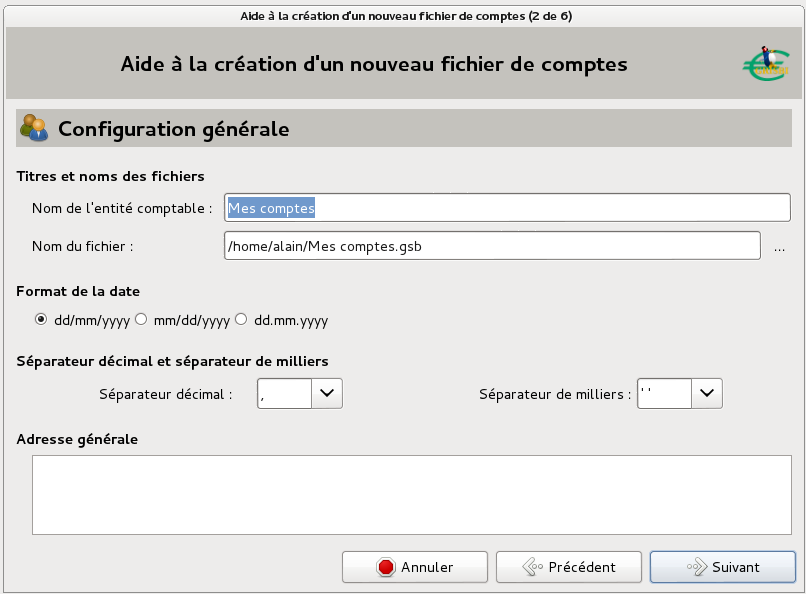
\includegraphics[scale=0.5]{image/screenshot/start_file_create}
\end{center}
\caption{Configuration générale du fichier de comptes}
\label{start-file-create-img}
\end{figure}
% image centre
\fi

\begin{enumerate} 
 \item choose the name of the accounting entity whose accounts you are managing, for example \og My accounts \fg{}, which can be chosen as the title of the Grisbi application home page,
\item enter the name of the accounts file with its complete tree; Grisbi defaults to the same name as the reporting entity, but you can change it
\item check the  \menu{Encrypt Grisbi} box if you wish to \gls{encrypt} the accounts file,
\item select the \indexword{date format}\index{date format} with one of the two buttons: dd/mm/yyyy for day/month/year, or  mm/dd/yyyy for month/day/year,
\item choose the decimal \indexword{separator}\index{separator} and the thousands from the drop-down lists,
 \item fill in the address (optional),
 \item  confirm with the  \menu{Forward} button;
\end{enumerate}

\item selection of the base \indexword{currency}\index{currency} :
\begin{enumerate} 
 \item click on the chosen currency in the list,
\item check the "include obsolete currencies" box if you also want to display old currencies,
\item confirm with the \menu{Forward} button;
\end{enumerate}

\item selection of the  \indexword{list of categories}\index{catgories !types} you will use :
\begin{enumerate} 
 \item click on your desired category, either the \menu{Standard category list} or the \menu{Empty list} \footnote{\strong{Translators Note:} Users installing the program on a system with a French Language interface will find different categories are offered including some for business users} 
\item check the \menu{Display foreign category sets} box to check if other categories are available\footnote{\strong{Translators Note:} This option is mainly for the benefit of users of a computer system with the French Language interface who will then be shown the two English categories mentioned in the previous step}
\item confirm with the \menu{Forward} button;
\end{enumerate}

\item Enter details of \indexword{banks}\index{banques !définition} holding your accounts :
\begin{enumerate} 
 \item click  \menu{Add} to define a bank; fill in the details of the bank (name, bank code, etc.), then confirm with the \menu{Add} to add the bank,
\item select a bank from the list and click the \menu{Remove} button to delete a bank, then confirm in the window that opens,
\item repeat actions a and b as many times as necessary,
\item  confirm with the \menu{Forward}  button to go to the next step, \menu{Creating a new account} ;
\end{enumerate} 

\item configuration completed: the configuration of the accounts file is complete, and this window offers you to choose one of the two methods of creating your first account
\ifIllustration compte\refimage{start-account-choice-img} :
\else compte :
\fi

\ifIllustration
% image centre
\begin{figure}[ht]
\begin{center}
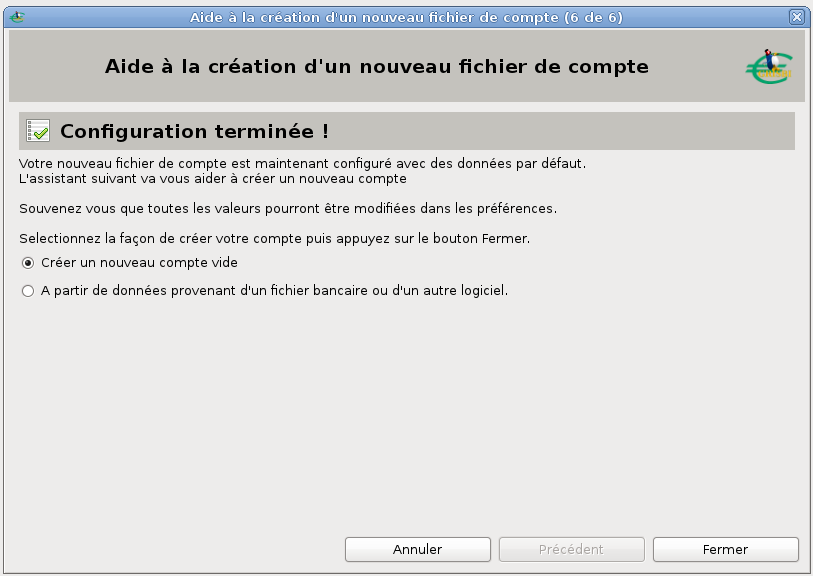
\includegraphics[scale=0.5]{image/screenshot/start_account_choice}
\end{center}
\caption{Choix du premier compte}
\label{start-account-choice-img}
\end{figure}
% image centre
\fi

\begin{itemize}
\item \menu{Create a new empty account} : if you check this line, then if you confirm with the \menu{Close} button, this window closes and the new account creation wizard starts. See  \vref{accounts-new}, \menu{Creating a new account},  which fully describes this procedure, then return to this page ;

\item \menu{From data from a bank file or other software} : if you check this line and then confirm with the \menu{Close} button ,  this window closes and the Import Data Wizard of a file account by Grisbi starts. See the \vref{move-import-importinit} section, \menu{Importing Account Files from Another Programme into Grisbi}, which fully describes this procedure, then return to this page.
\end{itemize}
\end{enumerate}

% tiquette du paragraphe suivant, pour que les liens hypertexte dans account.tex et QIF.tex  arrivent bien dessus
\label{start-newfile-end}

\textit{\textbf{In one way or another}}, you have now created your accounts file, as well as the first account of this file.

%espace pour changement de thme
\vspacepdf{5mm}

If you want to create other accounts now, select the \menu{Edit - New Account} to create another account (see the \vref{accounts-new}, \menu{ Creating a new account} section).

%espace pour changement de thme
\vspacepdf{5mm}

Otherwise, you can start using the account you just created or the one from which you just imported the data.

% espace avant Attention ou Note  : 5 mm
\vspacepdf{5mm}

\strong{Warning} : in general, it is inadvisable to have accents or spaces in the names of directories and files used by Grisbi. If so, rename them now. For example, spaces can be replaced by underscores (\underline{ }).

% saut de page pour titre solidaire
\newpage


\section{Saving your accounts file\label{start-save}}

Your operations are not written as you enter them as they might be in other software; you must therefore save your account file before exiting. Do not worry, Grisbi warns you if you have not done so.

You can configure the options for saving the account file in the  \menu{ Edit - Preferences} menu, see the section \vref{setup-general-files-manage}, \menu{Managing Account Files.}.


\section{Import from other personal accounting software}

See the \vref{move-import-importinit} section to import account files from another program into Grisbi. For the moment, Grisbi supports \gls{Gnucash}, \gls{OFX}, \GLS{CSV} and \GLS{QIF} formats.



\myclearemptydoublepage

%%%%%%%%%%%%%%%%%%%%%%%%%%%%%%%%%%%%%%%%%%%%%%%%%%%%%%%%%%%%%%%%%
% Contents : The home chapter
% $Id : grisbi-manuel-home.tex, v 0.4 2002/10/27 Daniel Cartron
% $Id : grisbi-manuel-home.tex, v 0.5.0 2004/06/01 Loic Breilloux
% $Id : grisbi-manuel-home.tex, v 0.6.0 2011/11/17 Jean-Luc Duflot
% some of its content was in menus chapter :
% $Id: grisbi-manuel-menus.tex, v 0.5.0 2004/06/01 Loic Breilloux
% $Id : grisbi-manuel-home.tex, v 0.8.9 2012/04/27 Jean-Luc Duflot
% $Id : grisbi-manuel-home.tex, v 1.0 2014/02/12 Jean-Luc Duflot
%%%%%%%%%%%%%%%%%%%%%%%%%%%%%%%%%%%%%%%%%%%%%%%%%%%%%%%%%%%%%%%%%

\chapter{Opening screen\label{home}}

\strong{Translators Note:} This chapter is currently under revision by {Jean-Luc \familyname{Duflot}}\footnote{email \urlJeanLucDuflotEmail{} Github site \urlJeanLucGit{}} which is fortunate as the user interface is not quite as described by this version.  Differences are highlighted in the text. In addition until the other chapters are translated many of the cross references lead to dead-ends at the moment.

When the application starts, Grisbi displays this
\ifIllustration opening screen \refimage{home-img} page.
\else d'accueil.
\fi
This opening screen can be accessed at any time by clicking on the  \menu{Accounts} tab. 

You can view the Grisbi window in full screen display \indexword{full screen mode}\index{affichage !plein écran}\index{plein écran !affichage} using the function key \key{F11}, and toggle between full screen and normal mode with the same key.

\ifIllustration
% image centrée
\begin{figure}[htbp]
\begin{center}
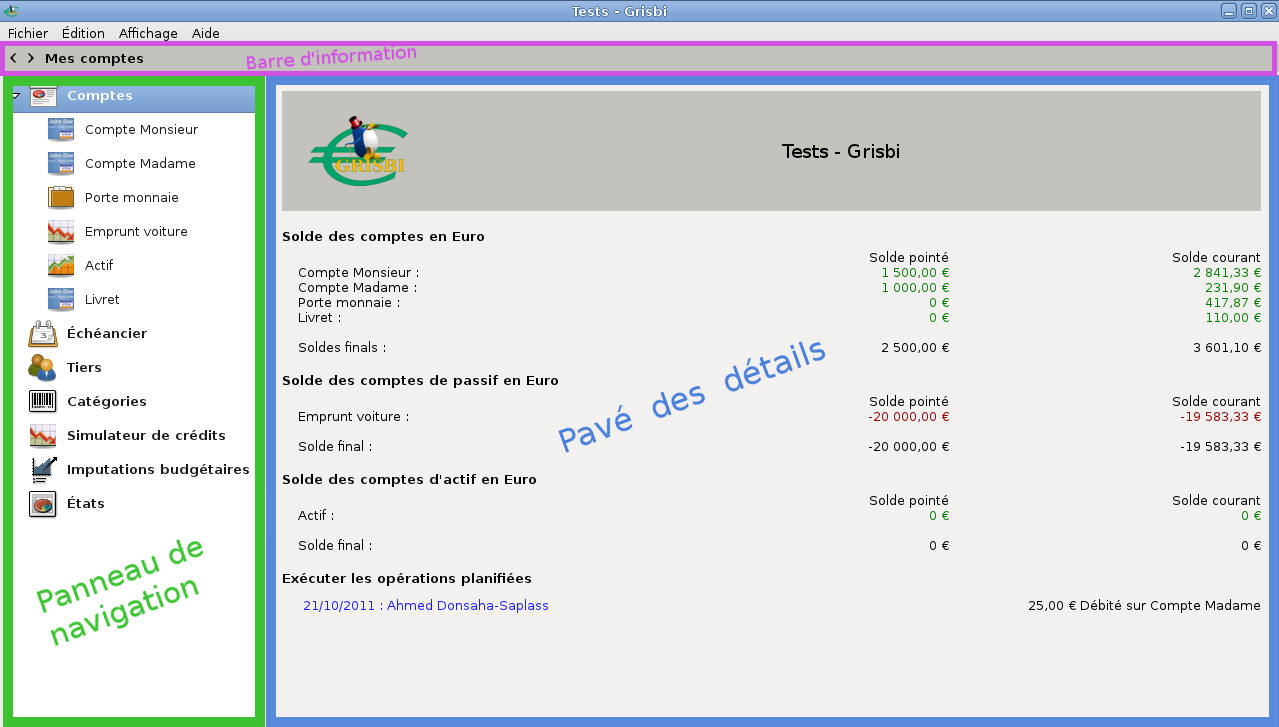
\includegraphics[scale=0.35]{image/screenshot/home}
\end{center}
\caption{Accounts summary page}
\label{home-img}
\end{figure}
% image centrée
\fi

All Grisbi screens have the same general appearance. It displays a menu bar that gives access to most of Grisbi's important features, and three main areas:

\begin{itemize}
	 \item the information bar, under the menu bar;
	 \item the navigation panel;
	 \item the main screen area.
\end{itemize}

\ifIllustration 
These three zones, specific to Grisbi, are outlined in different colors in the figure to identify them \refimage{home-img}.
\else
\fi

\section{Information bar\label{home-synthesis}}

The information bar displays the name of the current tab displayed, and can display, to the far right, the current balance if one of the accounts is selected for display in the main screen area.

% espace pour changement de thème
\vspacepdf{5mm}

To select one of the tabs displayed in the navigation panel click one or more times on one of the two small triangles on the top left of the panel.  The items displayed are : \menu{Accounts}, \menu{Scheduler}, \menu{Payees}, \menu{Credits simulator}, \menu{Categories}, \menu{Budgetary lines} and \menu{Reports}.  If the \menu{Accounts} and \menu{Reports} items have been expanded to display their sub categories these will also be displayed one by one.

% Pas de commande au clavier pour cette fonction
\textbf{Note} : These triangle symbols can be replaced, depending on the theme of the desktop environment or window manager you are using, by other characters such as +, -,>, <, and so on.

% espace pour changement de thème
\vspacepdf{5mm}
The content of the selection is displayed in the main screen area.

% espace pour changement de thème
\vspacepdf{5mm}
These features can be used instead of clicking directly in the navigation panel when the Information Bar window width is reduced to zero and you can not access it directly.


\section{Navigation panel\label{home-accounting}}

The navigation pane displays in bold the list of tabs:  \menu{Accounts}, \menu{Scheduler}, \menu{Payees}, \menu{Credits simulator}, \menu{Categories}, \menu{Budgetary lines} et \menu{Reports}. By clicking on the small black triangle to the left of the  \menu{Accounts} or \menu{Reports} tabs,  you can scroll or roll up the list of their sub-tabs. You can change the order of tabs and sub-tabs by clicking on one of them and dragging it up or down the list.

\textbf{Note} : These triangles can be replaced, depending on the theme of the desktop environment or window manager you are using, by other characters such as +, -,>, <, and so on.

% espace pour changement de thème
\vspacepdf{5mm}

You can select one of these tabs or sub-tabs by clicking on its name. You can also move the selection in this list of tabs and sub-tabs with the \key{Up Arrow}, \key{Down Arrow}, \key{Page Up} ou \key{Page Down} keys, or with the mouse wheel. 

% espace pour changement de thème
\vspacepdf{5mm}
The content of the selection is displayed in the main screen area.

% espace pour changement de thème
\vspacepdf{5mm}
You can reduce or enlarge the width of the navigation panel by clicking on the thin vertical bar between this panel and the main screen area, and moving it. If the width of the window has been reduced to zero, or enlarged to the maximum of the width of the Grisbi window, the thin vertical bar may be to the left or to the right of the window.  Locate this and slide it back to the desired location.

% espace pour changement de thème
\vspacepdf{5mm}

The \indexword{context menus}\index{context menus},  accessible by a right-click of the mouse, are available on the elements of this panel and offer the following functions::

\begin{itemize}
	 \item On \menu{Accounts} :
		\begin{itemize}
			 \item \menu{New account} ;
		\end{itemize}
	 \item On any account : 
		\begin{itemize}
			 \item \menu{New account},
			 \item \menu{Remove this account} ;
		\end{itemize}
	 \item On \menu{Payees} :
		\begin{itemize}
			 \item \menu{New payee},
			 \item \menu{Delete selected payee},
			 \item \menu{Edit selected payee},
			 \item \menu{Manage payees},
			 \item \menu{Remove unused payees} ;
		\end{itemize}
	 \item On \menu{Categories} : 
		\begin{itemize}
			 \item \menu{New category},
			 \item \menu{Delete selected category},
			 \item \menu{Edit selected category},
			 \item \menu{Import a file of categories (.csgb)},
			 \item \menu{Export the list of categories (.csgb)} ;
		\end{itemize}
	 \item On \menu{Budgetary lines} :
		\begin{itemize}
			 \item \menu{New budgetary line},
			 \item \menu{Delete selected budgetary line},
			 \item \menu{Edit selected budgetary line},
			 \item \menu{Import a file of budgetary lines (.isgb)},
			 \item \menu{Export the list of budgetary lines (.isgb)} ;
		\end{itemize}
	 \item On \menu{Report} : \menu{New report} ;
	 \item On any report : 
		\begin{itemize}
			 \item \menu{New report},
			 \item \menu{Remove this report}.
		\end{itemize}
\end{itemize}

\ifIllustration
\else
% saut de page pour titre solidaire
\newpage
\fi


\section{Details window\label{home-details}}

The main screen area displays all the details on the tabs or sub-tab selected by the Information Bar or Navigation Panel. This is the main work area of Grisbi.
You can reduce or enlarge its width by clicking on the thin vertical bar between this window and the navigation panel, and dragging it. If the width of the this panel has been reduced to zero or enlarged to the maximum of the width of the Grisbi window, the thin vertical bar may be to the left or to the right of the window.  Locate this and slide it back to the desired location.
 
\subsection{The summary screen\label{home-details-homepage}}

To return to the opening screen which provides an overview of the entire accounts file, select the Accounts tab; the main screen area then displays, from top to bottom:

\strong{Translators Note:} This section needs revision as the user interface is slightly different from this translation of the original French.

\begin{itemize}
	 \item in a box on a gray background, the \menu{Grisbi} icon on the left and on the right the \indexword{title}\index{title display !titre}\index{home page !page d'accueil} of the accounts file you currently have loaded, in the form  \og assigned name - Grisbi\fg{} ; ??you can define this name in one of three ways the \menu{Edit preferences} menu (see the paragraph \vref{setup-display-addresses-titles}, \menu{Titles})?? ; this can be useful if you manage multiple accounting entities:

		\begin{itemize}
			 \item The \menu{Accounting Entity} : This is the name you use to identify the type of account e.g. \og My Accounts \fg{} or \og Business\fg{}, which you entered when the account file was created; you can edit it here in the   \menu{Account Name field} ; this can be useful if you manage multiple  \indexword{accounting entities}\index{entité comptable}, 
			 \item The \menu{Account holder} :the name of the owner (or  account manager) of the last account accessed; if the holder is not defined in the account properties, Grisbi displays the name of this account,
			 \item le \menu{Accounts file name} :  This is the name of the file in the current directory, in the form  \file{name\_of\_\_your\_file.gsb}, and this is the default choice;
		\end{itemize}
		
	 \item for each currency separately, for all accounts and \indexword{groups of accounts}\index{groupe de comptes},  under the label \menu{Reconciled balance} and \menu{Current balance} :
		\begin{itemize}
			 \item the balance of the bank and cash accounts, the partial balance of the groups of accounts and their Global balance,
% saut de ligne pour indentation correcte de la note dans la liste

			 \textbf{Note} : you can adjust the display order of the partial balances of the account groups (see the section \vref{setup-general-home-partBalance}, \menu{Partial balances of the list of accounts}).			 
			 \item the balance of the liability accounts and their final balance,
			 \item the balance of the asset accounts and their final balance;
		\end{itemize}
	\item the \indexword{alerts from automatically scheduled entries}\index{alerte !opération planifiée} with their date, wording and amount, according to the choices made in the \menu{Edit - Preferences menu} (see th section \vref{setup-general-planned}, \menu{Timeline}) ;
	\item the list of accounts whose balance has fallen below the  \menu{minimum authorized balance} ;
	\item the list of accounts whose balance has fallen below the  \menu{required Minimum Balance}.
\end{itemize}

% espace avant Attention ou Note  : 5 mm
\vspacepdf{5mm}


\textbf{Note} : For definitions of \menu{Minimum Allowable Balance} and \menu{Desired  minimum balance}, see the \vref{accounts-properties}, \menu{Account Properties} section.

% espace pour changement de thème
\vspacepdf{5mm}

The account labels are displayed in black; as the mouse moves over any of the entries, this colour changes to gray.
A balance greater than the desired Minimum Balance is displayed in dark green; as the mouse cursor moves over the line, its colour changes to light green.


The account labels are displayed in black{\couleur} ; as the mouse cursor moves over the line of one of these, its colour changes to gray {\couleur}.
A balance greater than the  \menu{desired Minimum Balance}  is displayed in dark green {\couleur} ; as the cursor moves over the line, its colour changes to light green {\couleur}.



A balance less than the \menu{Minimum Balance Required} and greater than the \menu{Minimum Balance authorized} is displayed in orange{\couleur} ; as the pointer passes on its line, this color changes to light orange{\couleur}.
A balance less than the  \menu{Minimum Authorized Balance}  is displayed in red{\couleur} ; as the pointer passes over its line, this color changes to light red{\couleur}.

When you move the mouse pointer over the line of an account, any color change indicates that if you click (right or left) with the mouse, the records contained in the highlighted account is displayed, as if the account had been selected with the information bar or navigation panel.

A partial balance can be specified for a group of accounts  If defined this is displayed in black{\couleur}.If it is negative, it may appear in dark red{\couleur}, (see  \vref{setup-general-home-partBalance}, \menu{Partial balances for a list of accounts}). A partial balance line does not change color when the mouse pointer is over it, because you can not view the individual entries for of an group of accounts.

% espace pour changement de thème
\vspacepdf{5mm}
You can configure certain aspects of the display of this home page in the \menu{Edit - Preferences - Main - Main Page} on the Menu Bar or in the \menu{Properties} tab of each account :
\begin{itemize}
	 \item \menu{\indexword{Fonts}\index{polices}, \indexword{logo}\index{logo} et \indexword{coulours}\index{couleurs}} : section \vref{setup-display-logo} ;
	 \item \menu{?? Securities ??} : section \vref{setup-display-addresses-titles} ;
	 \item \menu{Calculation of balances} : paragraph \vref{setup-general-home-balance} ;
	 \item \menu{Partial balances from the list of accounts} : paragraph \vref{setup-general-home-partBalance} ;
	 \item \menu{Scheduler alerts} : section \vref{setup-general-planned} ;
	 \item Accounts below the \menu{\indexword{Minimum authorised balance}}\index{solde !minimal autorisé} : section \vref{accounts-properties} ;
	 \item Accounts below the \menu{\indexword{desired Minimum Balance}}\index{solde !minimal voulu} : section  \vref{accounts-properties}.
\end{itemize}

In particular, if you find a spelling error in this page, you can correct it: see the paragraph \vref{setup-general-home-final}, \menu{?? Pluriel de final ??} !

\ifIllustration
% saut de page pour paragraphe solidaire
\newpage
\fi

\section{menu bar\label{home-menus}}

As in many graphics applications, most of Grisbi's important features are accessible through the menus in the \indexword{Menu Bar}\index{barre de menus}. The features are detailed below.


\subsection{Menu \menu{Fichier}\label{home-menus-file}}

This menu includes the following functions :

>> CHECKED TO HERE  use the example file <<

%New account file: 
%Open: 
%Latest files:
%Save: 
%Save As: 
%Import a file: 
%Export to QIF / CSV file: 
%Create an archive: 
%Export an archive to a GSB / QIF / CSV file: 
%Debug the account file: 
%Make the account file anonymous: 
%Make the QIF file anonymous: 
%Debug mode: 
%Close: 
%Leave: Grisbi farm; 

\begin{itemize}
	\item \menu{Nouveau fichier de comptes} : creates a new account file; the current file is closed and a new empty file is created with an empty account (shortcut key \key{Ctrl}\key{N}),  see the \vref{start-newfile} section ; not to be confused with the creation of a new account;
	\item \menu{Ouvrir} : open an accounts file  (shortcut key  \key{Ctrl}\key{O}) ;
	\item \menu{Derniers fichiers} : displays the list of the last n files opened with Grisbi (only if there have been several); this number is configurable in the \menu{Edition - Préférences}, see the \vref{setup-general-files-manage}, \menu{Gestion des fichiers de compte} section ;
	\item \menu{Enregistrer} : Saves the current account file  (shortcut key \key{Ctrl}\key{S}) ;
	\item \menu{Enregistrer sous} : opens a file manager to save the current accounts file with the name and location of your choice; Grisbi defaults to the current directory, the name of the current accounts file, with the \file{.gsb} extension ;
	\item \menu{Importer un fichier} :starts the file import wizard of another software; see  \vref{move-import-importinit} ;
	\item \menu{Exporter vers un fichier QIF/CSV} :starts the Export Account File Wizard; see \vref{move-export} ;	
	\item \menu{Créer une archive} : starts the archive creation wizard; see \vref{datamanagement-history-new} ;	
	\item \menu{Exporter une archive vers un fichier GSB/QIF/CSV} : starts the archive export wizard; see \vref{datamanagement-history-export} ;
	\item \menu{Déboguer le fichier de compte} :Starts the debug wizard for this file, which will help you look for inconsistencies in your account file; see  \vref{maintenance-file-debug} ;
	\item \menu{Rendre anonyme le fichier de comptes} :starts the wizard that produces an anonymous copy of your account file; this file can be attached to a bug report; see \vref{maintenance-file-anonymous} ;	
	\item \menu{Rendre anonyme le fichier QIF} :  starts the wizard that produces an anonymous copy of this file; this file can be attached to a bug report; see \vref{maintenance-QIF-anonymous} ;	
	\item \menu{Mode de débogage} : puts Grisbi in debug mode, which creates a log file of events; see \vref{maintenance-debug-mode} ; 	
	\item \menu{Fermer} : closes the current accounts file; Grisbi offers to save it if you have not already done it (keyboard shortcut \key{Ctrl}\key{W}) ;
	\item \menu{Quitter} : ferme Grisbi ; Grisbi prompts you to save the account file if you have made any changes (raccourci-clavier \key{Ctrl}\key{Q}).
\end{itemize}


\subsection{Menu \menu{Édition}\label{home-menus-edit}}

Ce menu comprend les fonctions suivantes :

%itemize
%Edit operation: see transactions-modify section, Editing an operation;
%New operation: see transactions-new section, Entering a new transaction;
%Delete an operation: see transactions-delete section, Deleting an operation;
%Use the selected operation as a template: see transactions-model section, Operation selected as template;
%Clone the operation: see transactions-duplicate section, Cloning an operation;
%Convert to scheduled operation: see the transactions-schedule section, Converting an operation to a planned operation;
%Move the operation to another account: see the transactions-move section, Moving an operation to another account;
%New account: see accounts-new section, Creating a new account;
%Delete the current account: see the accounts-delete section, Deleting an account;
%Preferences:.
%itemize

\begin{itemize}
	\item \menu{Editer l'opération} : see \vref{transactions-modify}, \menu{Modification d'une opération} ;
	\item \menu{Nouvelle opération} : see \vref{transactions-new}, \menu{Saisie d'une nouvelle opération} ;
	\item \menu{Supprimer une opération} : see \vref{transactions-delete}, \menu{Suppression d'une opération} ;
	\item \menu{Utiliser l'opération sélectionnée comme modèle} : see \vref{transactions-model}, \menu{Opération sélectionnée comme modèle} ;
	\item \menu{Cloner l'opération} : see \vref{transactions-duplicate}, \menu{Clonage d'une opération} ;
	\item \menu{Convertir en opération planifiée} : see \vref{transactions-schedule}, \menu{Conversion d'une opération en opération planifiée} ;
	\item \menu{Déplacer l'opération vers un autre compte} :see \vref{transactions-move}, \menu{Déplacement d'une opération vers un autre compte} ;
	\item \menu{Nouveau compte} : see \vref{accounts-new}, \menu{Création d'un nouveau compte} ;
	\item \menu{Supprimer le compte courant} :see \vref{accounts-delete}, \menu{Suppression d'un compte} ;
	\item \menu{Préférences} :  allows you to configure Grisbi; see the \vref{setup}, \menu{Configuration de Grisbi} chapter.
\end{itemize}


\subsection{Menu \menu{Affichage}\label{home-menus-display}}

This menu includes the following functions : 



\begin{itemize}
	 \item \menu{Montrer le formulaire de saisie d'opérations} ; 
	 \item \menu{Montrer les opérations rapprochées} (raccourci-clavier \key{Alt}\key{R}) ;
	 \item \menu{Montrer les lignes d'archives} (raccourci-clavier \key{Altl}\key{L}) ;
	 \item \menu{Montrer les \indexword{comptes clos}}\index{compte !clos} ;
	 \item \menu{Montrer une ligne par opération} ;
	 \item \menu{Montrer deux lignes par opération} ;
	 \item \menu{Montrer trois lignes par opération} ;
	 \item \menu{Montrer quatre lignes par opération} ;
	 \item \menu{Réinitialiser la largeur des colonnes} ; permet de remettre les colonnes des listes d'opérations à leur largeur d'origine.
\end{itemize}


\subsection{Menu \menu{Aide}\label{home-menus-help}}

>>> DONE TO HERE



Most of the choices in this menu give links to websites. In order for these links to work, you must have specified to Grisbi the navigation software (or browser) that you wish to use, in the \menu{Édition - Préférences} (see \vref{setup-general-programs}, \menu{Programmes}). Le menu \menu{Aide}  includes the following choices :

\begin{itemize}
	\item \menu{Manuel} : opens your browser to the \og Grisbi User Manual page \fg{} (shortcut key  \key{Ctrl}\key{H}) ;
	\item \menu{Démarrage rapide} : opens your browser to the \og Grisbi Quick Start page \fg{} ;
	\item \menu{Traduction} : opens your browser to the \og Translate Grisbi \fg{}, to help us to widen the internationalization of Grisbi ;
	\item \menu{À propos de Grisbi} : displays the program information box: you will find details about the version, the link to Grisbi's site, the acknowledgements page (contributors to the project) and the user license ;
	\item \menu{Site Web de Grisbi} : opens your browser to the \lang{Grisbi}\footnote{\urlGrisbi{}} web site ;
	\item \menu{Signaler une anomalie} : opens your browser to the \lang{Grisbi Bug Tracker page}\footnote{\urlBugTracker{}} to allow you to report a bug that you have discovered. You can also follow on this page the evolution of the corrections made to the reported bugs;
	\item \menu{Astuce du jour} : opens a dialog box that displays a tip of use, different each time Grisbi starts; you can successively display all the tips, and choose whether or not the display of the tip of the day when starting Grisbi. To remove or reactivate the tip of the day, see \vref{setup-display-messages-trick}, \menu{Astuce du jour}.
\end{itemize}


\section{Raccourcis-clavier\label{home-shortcuts}}


Keyboard shortcuts make it easy to enter data and navigate through Grisbi's windows, avoiding the need to move and click. By using the ones corresponding to the most common manipulations for you, you improve your ergonomics \indexword{ergonomie}\index{ergonomie} by limiting the important movements of your arms.
 
Grisbi has a number of keyboard shortcuts, presented here according to different themes (see also  \vref{introduction-manual-conventions}, \menu{Conventions typographiques du présent manuel}).
%introduction-manual-conventions, Typographical Conventions in this manual).

\subsection{Application et fichiers}

\begin{itemize}
	\item New accounts file : \key{Ctrl}\key{N}
	\item Open an account file : \key{Ctrl}\key{O}
	\item Register the account file : \key{Ctrl}\key{S}
	\item Close the account file : \key{Ctrl}\key{W}
	\item Close Grisbi : \key{Ctrl}\key{Q}
\end{itemize}


\subsection{Panneau de navigation}

\begin{itemize}
	\item Select a tab or account: \key{ Arrow Up}, \key{Arrow Down}, \key{Page Up} ou \key{Page Down}
\end{itemize}

\subsection{List of operations and planned operations}

\begin{itemize}
	\item Select an operation: \key{Enter}
	\item Move selection:\key{Arrow Up} ou \key{Arrow Down}
	\item New operation:  \key{Enter} on empty line, or \key{Ctrl}\key{T}
	\item Modify an operation: \key{Enter}
	\item Delete an operation: \key{Delete} ;
	\item Point or detach an operation:\key{Ctrl}\key{P}
	\item Reconcile or unhook an operation: \key{Ctrl}\key{R}
	\item Show or hide archival lines: \key{Altl}\key{L}
\end{itemize}


\subsection{Entry form }

\begin{itemize}
	\item The \key{Enter} is configurable : it can be set to either move in the input form, or to validate the entry
	\item Move to the next field : \key{Tab} (depending on your configuration choice)
	\item Cancel the current entry : \key{Esc}
	\item Accept auto-complete : \key{Tab} or \key{Enter} (depending on your configuration choice)
	\item  Euro symbol : \key{AltGr}\key{e}
\end{itemize}

\subsection{Drop down lists}

\begin{itemize}
	 \item Open a list : \key{Page Down} ou \key{Down Arrow}
	 \item Move in the list : \key{Up Arrow}, \key{Down Arrow}, \key{Page Up} or \key{Page Down}
	 \item Validate a choice within a list: \key{Enter}
	 \item Currencies, ??exercises?? and methods of payment:
		\begin{itemize}
			\item open list : \key{Space} ; 
			\item move in the list: \key{Up Arrow} ou \key{Down Arrow} ;
			\item validate the item in the list : \key{Space}.
		\end{itemize}
\end{itemize}


\subsection{Dates entered on the calendar}

itemize
Opens a calendar (on the date field): Ctrl Enter
Closes the calendar without changing the date: Esc
Validate the selected date: Enter
Next or previous day: + or -, Right Arrow or Left Arrow
Previous or next week: Arrow Up or Arrow Down
Previous or next month: Page Up or Page Down
First day or last day of the month: Start or End
itemize

\begin{itemize}
	\item Opens a calendar (on the date field) : \key{Ctrl}\key{Enter}
	\item Closes the calendar without changing the date : \key{Esc}
	\item Validate the selected date : \key{Enter}
	\item Next or previous day : \key{+} ou \key{-}, \key{Right Arrow} or \key{Left Arrow}
	\item Previous or next week : \key{Up Arrow} or \key{Down Arrow}
	\item Previous or next month : \key{Page Up} or \key{Page Down}
	\item First day or last day of the month : \key{Start} or \key{End}
\end{itemize}


\subsection{Dates entered on keyboard }

\begin{itemize}
	\item Next or previous day : \key{+} ou \key{-}
	\item Previous or next week : \key{Shift} \key{+} ou \key{Majuscule} \key{-}
	\item Previous or next month : \key{Page Up} ou \key{Page Down}
	\item Previous or Next Year : \key{Shift} \key{Page Up} ou \key{Shift} \key{Page Down}
	\item Validate the selected date \key{Enter}
\end{itemize}


\subsection{Payees, categories, budget allocations, credit simulator, historical data and forecasts}

\begin{itemize}
	\item Move selection : \key{Up Arrow}, \key{Down Arrow}, \key{Page Up} ou \key{Page Down}
%Ces raccourcis ne fonctionnent plus :
%	\item afficher les sous-catégories ou sous-imputations budgétaires (sur une catégorie ou une imputation budgétaire) : \key{Espace} ;
%	\item afficher les opérations des sous-catégories ou sous-imputations budgétaires (sur une sous-catégorie ou une sous-imputation budgétaire) : \key{Espace}.
\end{itemize}


\subsection{States and Configuration}

\begin{itemize}
	\item Select another tab : \key{Up Arrow}, \key{Down Arrow}, \key{Page Up}, \key{Page Down}
	\item Navigate between the tab panel and the different options in the settings panel : \key{Tab}, \key{Up Arrow}, \key{Down Arrow}, \key{Left Arrow} et \key{Right Arrow}
\end{itemize}

\subsection{Help}

\begin{itemize}
	\item Open your browser on the Grisbi User Manual page \key{Ctrl}\key{H}
\end{itemize}














\myclearemptydoublepage

%%%%%%%%%%%%%%%%%%%%%%%%%%%%%%%%%%%%%%%%%%%%%%%%%%%%%%%%%%%%%%%%%
% Contents: The QIF chapter
% $Id: grisbi-manuel-QIF.tex, v 0.4 2002/10/27 Daniel Cartron
% $Id: grisbi-manuel-QIF.tex, v 0.5.0 2004/06/01 Loic Breilloux
% $Id: grisbi-manuel-QIF.tex, v 0.6.0 2011/11/17 Jean-Luc Duflot
% $Id: grisbi-manuel-QIF.tex, v 0.8.9 2012/04/27 Jean-Luc Duflot
% $Id: grisbi-manuel-QIF.tex, v 1.0 2014/02/12 Jean-Luc Duflot
%%%%%%%%%%%%%%%%%%%%%%%%%%%%%%%%%%%%%%%%%%%%%%%%%%%%%%%%%%%%%%%%%


\chapter{Export and import of accounts\label{move}}

You can not directly use data that has been created by other personal accounting applications in Grisbi, and vice versa. Because these applications work differently, their data is structured differently, so you need to convert their data structure before you can use it. 

This conversion can not be done at once on all data, but must be done separately for each account managed by the application. To convert each of these accounts, you must first \og export \fg{}them from the original application and then \og import \fg{} them into the destination application.

% espace avant Attention ou Note  : 5 mm
\vspacepdf{5mm}

\strong{Warning} :  do not confuse the \og accounts file \fg{}which contains all the data of all the accounts created for the management of an accounting entity (in Grisbi, this file has the \gls{extension} \file{.gsb}), and the \og account files\fg{}, which are files that contain only data from one account at a time, and created only to export or import that data from one accounting application to another. These \og account files  \fg{}  must have a  \gls{file format} (or extension) that must be compatible with the original application AND the destination application.
% espace après Attention ou Note  : 5 mm
\vspacepdf{5mm}

Grisbi currently supports \gls{Gnucash}, \gls{OFX}, \gls{CSV} and \gls{QIF} personal accounting data formats.

\section{Importing accounts from another accounting application\label{move-import}}

If you want to use account data that has been created
in another accounting application in Grisbi, you must first export each of the accounts of this application individually to a set of files, then import these same files into Grisbi.

\subsection{Export an account file from the other accounting application \label{move-import-exportinit}}

The first step is, in the originating personal accounting application, to export each account in a file in the chosen format. The chosen format must be compatible with the export formats supported by the original application \emph{and} compatible with import to Grisbi.

The export procedure is obviously different for each accounting application, so refer to its documentation. If you want to export all accounts, you will need to get as many files as you have accounts managed by the application.


\subsection{Importing account files from another accounting application to Grisbi\label{move-import-importinit}}

\textbf{Note} : Grisbi allows you to import one or more account files in one operation. Although you can import the account files one by one, it is important to import all the account files at the same time, so that Grisbi can recreate the links between the accounts, especially with regard to the transfer operations.
% espace après Attention ou Note  : 5 mm
\vspacepdf{5mm}

For more information on the \indexword{account types}\index{types de compte} that Grisbi can manage, see the \vref{accounts-type}, \menu{Grisbi account types} section.

You can define which date will be used for assigning a financial year to
each imported operation, see \vref{setup-general-import-financialyear}, \menu{Definition of Financial Year}.

When you import a file, Grisbi allows you to establish an association between a string of characters in this file and a payee. For example, all labels containing \og rent \fg{}  may be associated with a payee that represents your landlord. This must be configured in the \menu{Edit - Preferences } menu (see the \vref{setup-general-importLinks}, \menu{Associations for Import} section).

% espace pour changement de thème
\vspacepdf{5mm}

In the Grisbi \menu{File} menu, choose the option  \menu{Import
file\ldots{ }}, which opens the import wizard window. The import of the account files takes place in five steps :

\begin{enumerate}
	\item Launches the import assistant; confirm with the \menu{Forward} button;
	\item Selection of the account files to import :	
		\begin{enumerate}
			\item click the button \menu{Add file to import} button : a file manager window opens,	
			\item look for the directory where these account files are,
			\item select one or more account files (with the combination   \key{Ctrl}\key{Click} and \key{Shift}\key{Click}); you can also change the \gls{locale} (\gls{character encoding}) of the files to import from the \menu{Encoding} drop-down menu,
			\item validate the window to return to the account file selection window,
			\item when the desired files are checked, you can validate the selection with the \menu{Forward} button;
		\end{enumerate}		  
	\item Complete the import of the files: if everything went well, this window gives the list of the account files which will be imported; continue the import by confirming with the \menu{Forward} button;
	\item Review: you can review each account and choose the following actions \strong{Translators Note:} this paragraph has not been checked against Grisbi so could still contain translation errors \ifIllustration \refimage{QIF-import-files-setup-img} :
	% image centrée
	\begin{figure}[htbp]
	\begin{center}
	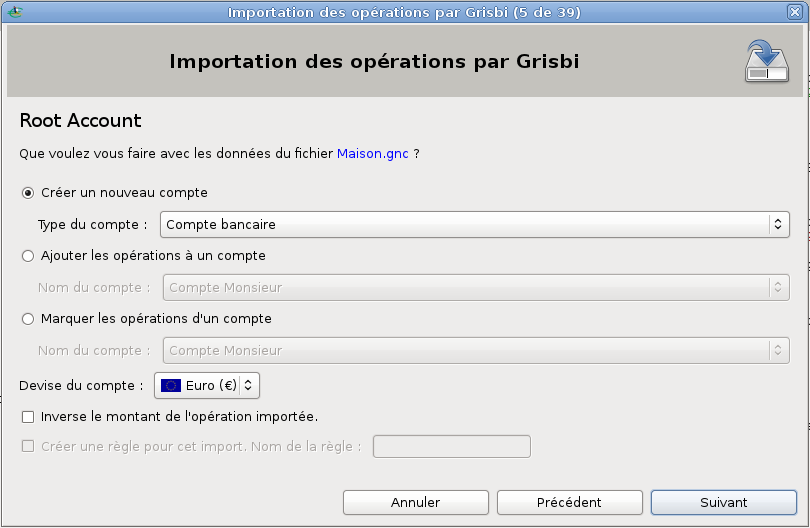
\includegraphics[scale=0.5]{image/screenshot/QIF_import_files_setup}
	\end{center}
	\caption{Setting up each imported account}
	\label{QIF-import-files-setup-img}
	\end{figure}
	% image centrée
	\else  :
	\fi
	
		\begin{itemize}
			\item create a new account,
			\item add a scheduled transaction to an account: If scheduled transactions are found within the specified time interval, a specific window opens to find out what you want to do: either merge these scheduled transaction with the corresponding imported entry, or add them imported transaction in addition to those (see \vref{setup-general-import-parameters}, \menu{Import Settings}),
			\item check the scheduled transactions : if there are \indexword{orphaned transactions}\index{opération !orpheline}  a window will open at the end of the import to know what you want to do: either add them or ignore them,
			\item set the currency of the account (or create a new one),
			\item   reverse the amount of the transaction (useful for credit card accounts for example),
			\item create a fast import rule if the file is in QIF or OFX format,
			\item when everything is correct, confirm the import with the \menu{Next} button;
		\end{itemize}
	
	 \item Confirm the end of the import: confirm with the \menu{Close} button.
\end{enumerate}

If, and only if you have created your account file just before this account data import, return to the end of the  \vref{start-newfile-end}, \menu{Creating a New Account File}. Go directly to the end of the account file creation process, at the paragraph beginning with \emph{In one way or another\ldots{ }}, which will prompt you to create other accounts right away.

%espace pour changement de thème
\vspacepdf{5mm}
Otherwise, you can start using the account you just created.

\section{Export accounts from Grisbi\label{move-export}}

If you want to use account data created by Grisbi in another accounting application, you must first export this data to files and then import them into the other application using these files. The file format chosen must be compatible with the export by Grisbi \emph{and} compatible with the import by the destination application.
 
In the \menu{File} menu select the \menu{Export accounts as QIF/CSV file\ldots{ }} that opens the Export Accounts Wizard. There are four steps to exporting accounts:

\begin{enumerate}
	\item Starting the assistant; this window indicates that, since the QIF and CSV file formats do not support currency, all transactions will be converted into the currency of their respective account; confirm with the \menu{Forward} button;
	\item Select the accounts to export by clicking in the corresponding box; confirm with the  \menu{Forward} button;
	\item For each account, define the name of the file, the destination directory and the export format, then validate with the \menu{Forward} button \ifIllustration \refimage{QIF-export-img} ;
	% image centrée
	\begin{figure}[t]
	\begin{center}
	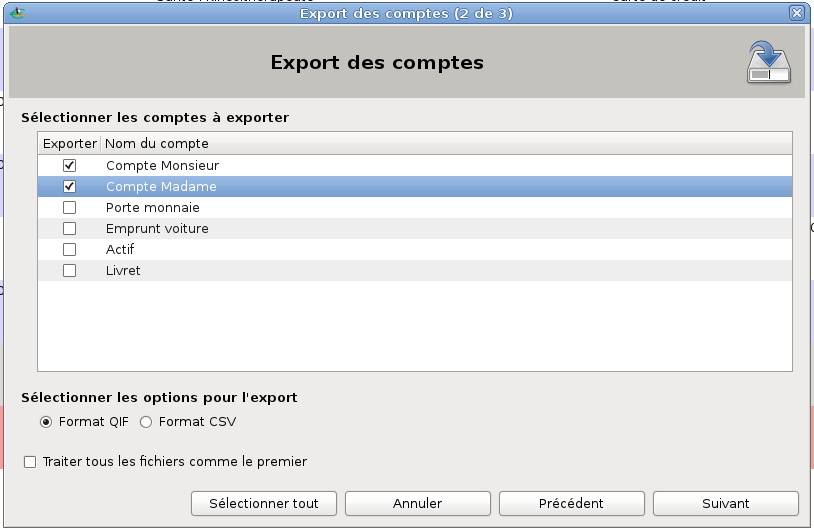
\includegraphics[scale=0.5]{image/screenshot/QIF_export}
	\end{center}
	\caption{Acount export}
	\label{QIF-export-img}
	\end{figure}
	% image centrée
	\else  ;
	\fi
	
	\item The completion of the export window is displayed; confirm with the \menu{Close} button.
\end{enumerate}

\strong{Warning}: in general, it is inadvisable to have accents or spaces in the names of directories and files used by Grisbi. If so, rename them now. For example, spaces can be replaced by underscores (\_).












\myclearemptydoublepage

%%%%%%%%%%%%%%%%%%%%%%%%%%%%%%%%%%%%%%%%%%%%%%%%%%%%%%%%%%%%%%%
% Contents : The data management chapter
% $Id : grisbi-manuel-datamanagement.tex, v 0.8.9 2012/04/27 Jean-Luc Duflot
% $Id : grisbi-manuel-datamanagement.tex, v 1.0 2014/02/12 Jean-Luc Duflot
%%%%%%%%%%%%%%%%%%%%%%%%%%%%%%%%%%%%%%%%%%%%%%%%%%%%%%%%%%%%%%%%%

\chapter{Data management\label{datamanagement}}

The data you enter into Grisbi must be carefully preserved and protected against accidental loss. Grisbi provides three tools to address this issue : \menu{Account file management}, \menu{Backups} and \menu{Archives}.

\section{Managing the account files\label{datamanagement-files}}

You can set the following management options:

\begin{itemize}
	\item automatically load last file on startup;
	\item automatically on exit;
	\item \indexword{Force saving}\index{enregistrement !forçage} of locked files ;
	\item \indexword{Encrypt}\index{fichier de comptes !chiffrement}\index{chiffrement !fichier de comptes} Grisbi file;
	\item\indexword{\gls{Compress}} Grisbi file\index{fichier de comptes !compression}\index{compression !fichier de comptes} ;
	\item Memorise last opened files.
\end{itemize}

All of these options are explained in detail and can be configured in the \menu{Edit - Preferences} menu (see \vref{setup-general-files-manage}, \menu{Managing Account Files}).


\section{Data management-backup\label{datamanagement-backup}}

In general, no matter what data you have on your computer's hard drive, you need to make backups of it, for the simple reason that \emph{any data storage system has a limited lifetime}. Making backups is designed to limit the risk of data loss. 

Grisbi allows you to make automatic backups of your accounts file. These backups should be stored in a special directory or a special \gls{partition} of your computer's disk, with backups of all your other data, which would then allow you to easily back up this directory or partition, preferably on different types of media, independent of the computer, and put in a safe place.

% espace avant Attention ou Note  : 5 mm
\vspacepdf{5mm}
\textbf{Note}:  take these tips seriously and do not take risks with your data, this can save you many setbacks\ldots
% espace après Attention ou Note  : 5 mm
\vspacepdf{5mm}

Grisbi can automatically save, in a directory to be defined, either a single backup file that is replaced regularly, or backup files that accumulate in this directory.
The backup files have a name of the form \file{name\_of\_file\_YYYYMMDDTHHMMSS.gsb}, where \emph{name\_of\_file} is the name of your accounts file, \emph{YYYYMMDD} is the date in year-month-days, \emph{T}  is a separator, and \emph{HHMMSS}  is the time in hours- minutes-seconds. This format is based on the ISO 8601 international date format, which permits, among other things, the automatic sorting in alphanumeric and chronological order in your backup directory.

%espace pour changement de thème
\vspacepdf{5mm}
Grisbi provides you the following backup options:

\begin{itemize}
	\item the creation of a single backup file, otherwise the backup files are added to their directory;
	\item the \indexword{\gls{compression} of the backup file}\index{fichier de sauvegarde !compression}\index{compression !fichier de sauvegarde}, to occupy less disk space;
	\item backup after opening the account file; 
	\item backup before saving the account file; 
	\item setting the interval between two backups, in minutes;
	\item setting the \indexword{backup directory}\index{répertoire de sauvegarde}\index{fichier de sauvegarde !répertoire}.
\end{itemize}

%espace pour changement de thème
\vspacepdf{5mm}
All of these options are described in detail and can be configured in the \menu{Edit - Preferences} menu (see \vref{setup-general-files-backup}, \menu{Backups}).


\section{Archives\label{datamanagement-history}}

%An archive is a little like \og placing in parentheses \fg{} some of the entries from all the accounts in your account file.

Entries inside an archive are no longer displayed and can no longer be processed, but are preserved. You can always unarchive an existing archive at any time to access its data. 

When you use Grisbi, you enter transactions into your different accounts. These operations are all stored in the computer's memory and hard disk, and a few of these are displayed on the screen. The display and processing of account entries consumes memory and microprocessor time.

As time goes by, there are more and more operations recorded, so their display and processing require more and more memory space and microprocessor time. Your computer (depending on its specification) will eventually start to run Grisbi more slowly. 

To limit this loss of performance in the display and the processing, in particular in report generation or in the search for information, Grisbi prompts you to choose a portion of your entries and to put them in an archive, that is, to set them apart so that they are not affected by future postings or operation.

Archiving can be manual or automated. Grisbi considers that beyond three thousand operations in an account, the entries become too slow, so on the one hand it warns you if you exceed this number of transactions and prompts you to manually archive a section of them. Alternatively, it can let you archive these three thousand transactions by automatically launching an assistant.

Whether you do an archiving manually or with the assistant, the counting process is then reset and Grisbi will offer you the same thing again after three thousand additional operations.



\subsection{Archives in the list of transactions\label{datamanagement-history-list}}

The \indexword{display of an archive}\index{archive !affichage} appears at the top of the list of operations for \emph{each account},  in the form of an operation line on a green{\couleur} background, indicating its date of creation, its name and its creation parameters. (dates and financial year or report name), as well as \ifIllustration the \indexword{ number of archived operations}\index{archive !nombre d'opérations} \emph{for the account displayed}, and the \indexword{total number of transaction}\index{opération !nombre total} in your accounts file\refimage{datamanagement-history-line-img}.

% image centrée
\begin{figure}[htbp]
\begin{center}
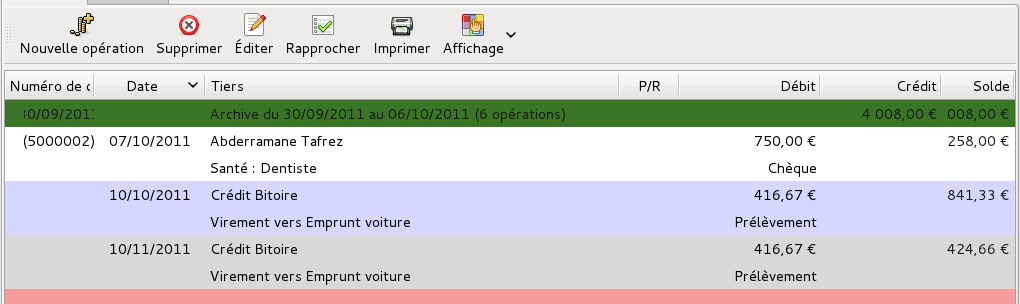
\includegraphics[scale=0.5]{image/screenshot/datamanagement_history_line}
\end{center}
\caption{Archive line displayed}
\label{datamanagement-history-line-img}
\end{figure}
% image centrée
\else the \indexword{ number of archived operations}\index{archive !nombre d'opérations} \emph{for the account displayed}, and the \indexword{total number of transactions}\index{opération !nombre total} in your accounts file.
\fi


You can show or hide all archive rows in the list of operations for all accounts by selecting the \menu{View - Show Lines Archive}, or by clicking the \menu{View} tool on the toolbar, and then click selecting \menu{Show Archive Lines} from its drop-down list.

If you want to view the operations inside an archive, you can open this archive by double-clicking on its line: after validation in the window that appears, the operations are displayed in the list.

\textbf{Note}: this is only an opening of the archive for display, and in no case this archive is deleted. The next time Grisbi is used, the green line of the archive will reappear at the top of the list for each account. For a true deletion of the archive, see the \vref{datamanagement-history-remove}, \menu{Deleting an archive} section.



\subsection{Creating and archive\label{datamanagement-history-new}}

To create an archive, follow these steps:

\begin{enumerate}
	\item in the menu bar, select \menu{File - Archive transactions\ldots{}} : The Archive Creation Wizard window is displayed; confirm with the \menu{Forward} button;
	\item in the following window, you can choose the operation selection mode to archive  \ifIllustration archiver\refimage{datamanagement-history-create-img}:
	% image centrée
	\begin{figure}[htbp]
	\begin{center}
	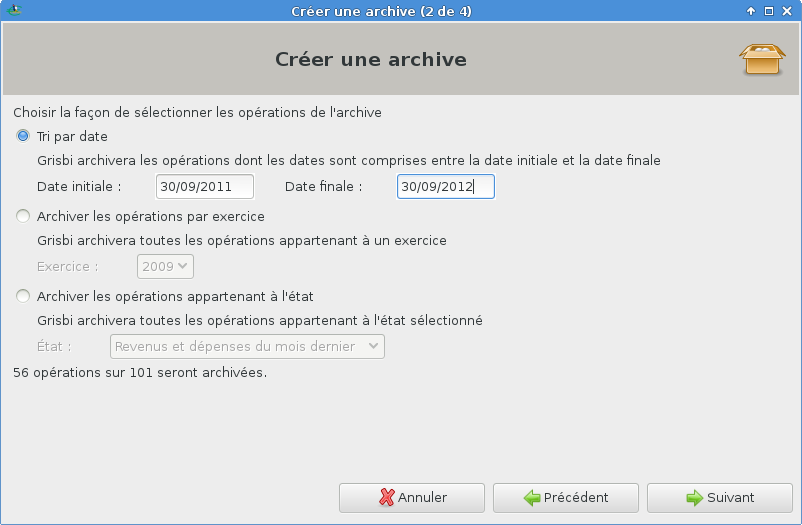
\includegraphics[scale=0.5]{image/screenshot/datamanagement_history_create}
	\end{center}
	\caption{Creating an archive}
	\label{datamanagement-history-create-img}
	\end{figure}
	% image centrée
	\else archiver :
	\fi
	
		\begin{itemize}
			\item \menu{Archive by Date}: enter the \menu{Initial date} and \menu{Final date} in the appropriate fields,
			\item \menu{Archive transactions by financial year}: Select an available year from the drop-down list,
			\item \menu{Archive transactions by report}: Select an available report from the drop-down list;
% saut de ligne pour indentation correcte de la note dans la liste

			\textbf{Note}: the last line in the window indicates either an error in entering these parameters, the number of transactions that will be archived and the total number of operations in your accounts file.  
		\end{itemize}
	\item confirm with the \menu{Forward} btton;
	\item in the next window, enter the name you want for this archive; confirm with the  \menu{Apply} button;
	\item the last window informs you that the archive has been created, and displays the \indexword{number of archived transactions}\index{archive !nombre d'opérations}, number of transactions and the total number of transactions of your accounts file;  \emph{all accounts taken together};  validate with the \menu{Back} button to create another archive, otherwise by the \menu{Close} button.
\end{enumerate}

\textbf{Note}: In case Grisbi has become slower after creating an archive, you can configure it to not load the close operations (R) on startup, in order to increase its speed, see the \ref{transactions-functions}, \menu{tool bar}).

% espace après Attention ou Note  : 5 mm
\vspacepdf{5mm}
The archive appears at the very top of the list of operations \emph{for each account} (see the \vref{datamanagement-history-list} section, \menu{Archives in the list of transactions}).


\subsection{Creation warning and automatic creation of archives\label{datamanagement-history-auto}}

When a certain number of registered transactions is reached, Grisbi can first of all warn you that this quantity of operations has not yet been archived, on the other hand automatically start the creation of an archive (see \vref{setup-general-archives-create}, \menu{warning and automatic creation}).

By clicking on the box labelled \menu{Automatically create an archive if necessary}, you enable the automatic archiving function.

With the label \menu{Warn if more transactions \ldots{ } are not archived}, you can set this number of operations. The default value is 3000.


\subsection{Parameters of an archive\label{datamanagement-history-parameters}}
You can consult the parameters that were defined during the creation of an archive, in the 
\menu{Edit - Preferences - Archives} menu. For this see the \vref{setup-general-archives-existing}, \menu{Existing Archives}.


\subsection{Editing an archive\label{datamanagement-history-modify}}

You can only \indexword{change the name of an archive}\index{archive !modification} in the \menu{Edit - Preferences } menu. For this see the \vref{setup-general-archives-remove}, \menu{Edit the archive} section.


\subsection{Deleting an archive\label{datamanagement-history-remove}}

You can \indexword{delete an existing archive}\index{archive !suppression} , in the menu \menu{Edit - Preferences} menu. There are two separate delete functions: deleting an archive while  \emph{retaining} its transactions,and deleting an archive while  \emph{deleting}  all its operations. For this see \vref{setup-general-archives-remove}, \menu{Edit the archive}. 


\subsection{Export an archive\label{datamanagement-history-export}}

Allows you to create a file containing the archive, in order to store it, or to use it in another Grisbi account file or in another accounting application. Exporting can only be done through \indexword{\gls{GSB}}\index{gsb}, \indexword{\gls{QIF}}\index{qif} or \indexword{\gls{CSV}}\index{csv}.

% espace avant Attention ou Note  : 5 mm
\vspacepdf{5mm}
\strong{Caution}: QIF and CSV file formats do not support currency, and all transactions will be converted to the currency of their respective account.
% espace après Attention ou Note  : 5 mm
\vspacepdf{5mm}



To export an archive, follow these steps:

\begin{enumerate}
	\item in the menu bar, select \menu{Export an archive to a GSB, QIF or CSV file ... } : the archive export wizard window is displayed; confirm with the \menu{Forward} button;
	\item a table displays the list of existing archives with their name and, as the case may be, their initial and final dates, their exercise or the name of the report; select the archive to export by checking the box in its line; confirm with the \menu{Forward} button;
	\item a file manager window is displayed; optionally modify the name of the file under which the archive will be exported, the folder where it will be saved and the format of the export file; confirm with the \menu{Forward} button;
	\item the last window informs you that the archive has been exported; confirm with the \menu{Close} button.
\end{enumerate}










\myclearemptydoublepage

%%%%%%%%%%%%%%%%%%%%%%%%%%%%%%%%%%%%%%%%%%%%%%%%%%%%%%%%%%%%%%%%%
% Contents : The accounts chapter
% $Id : grisbi-manuel-accounts.tex, v 0.4 2002/10/27 Daniel Cartron
% $Id : grisbi-manuel-accounts.tex, v 0.5.0 2004/06/01 Loic Breilloux
% some of its content was in tips chapter : 
% $Id : grisbi-manuel-tips.tex, v 0.4 2002/10/27 Daniel Cartron
% $Id : grisbi-manuel-accounts.tex, v 0.6.0 2011/11/17 Jean-Luc Duflot
% some of its content was in tips chapter :
% $Id : grisbi-manuel-tips.tex, v 0.5.0 2004/06/01 Loic Breilloux
% $Id : grisbi-manuel-accounts.tex, v 0.8.9 2012/04/27 Jean-Luc Duflot
% $Id : grisbi-manuel-accounts.tex, v 1.0 2014/02/12 Jean-Luc Duflot
% some of its content was in transactions chapter :
% $Id : grisbi-manuel-transactions.tex, v 0.8.9 2012/04/27 Jean-Luc Duflot
%%%%%%%%%%%%%%%%%%%%%%%%%%%%%%%%%%%%%%%%%%%%%%%%%%%%%%%%%%%%%%%%%

\chapter{Gestion des comptes\label{accounts} }

Note: This chapter is currently being translated by Bob Anderson 

\section{Liste des comptes\label{accounts-list}}


\section{Sélection d'un compte\label{accounts-selection}}

\section{Propriétés d'un compte\label{accounts-properties}}



\section{Création d'un nouveau compte\label{accounts-new}}



\section{Modification d'un compte\label{accounts-modify} }



\section{Suppression d'un compte\label{accounts-delete} }


\section{Types de compte de Grisbi\label{accounts-type}}

\subsection{Type compte bancaire\label{accounts-type-bank}}



\subsubsection{Compte bancaire, courant, d'épargne ou de carte bancaire à débit immédiat\label{accounts-type-bank-misc}}


\subsubsection{Compte de carte de crédit\label{accounts-type-bank-creditcard}}


\subsubsection{Compte d'attente\label{accounts-type-bank-waiting}}


\subsubsection{Compte d'avances\label{accounts-type-bank-advance}}



\subsection{Type compte de caisse\label{accounts-type-cash}}


\subsection{Type compte de passif\label{accounts-type-liabilities}}

\subsubsection{Compte d'emprunt\label{accounts-type-liabilities-loan}}


\subsubsection{Compte de carte bancaire à débit différé\label{accounts-type-cash-deferredCards}}


\subsection{Type compte d'actif\label{accounts-type-assets}}



\section{Conversion d'un compte en euros\label{accounts-switcheuro}}




\myclearemptydoublepage

%%%%%%%%%%%%%%%%%%%%%%%%%%%%%%%%%%%%%%%%%%%%%%%%%%%%%%%%%%%%%%%%%
% Contents : The transactions chapter
% $Id : grisbi-manuel-transactions.tex,v 0.4 2002/10/27 Daniel Cartron
% $Id : grisbi-manuel-transactions.tex, v 0.5.0 2004/06/01 Loic Breilloux
% some of its content was in tips chapter  : 
% $Id : grisbi-manuel-tips.tex, v 0.4 2002/10/27 Daniel Cartron
% $Id : grisbi-manuel-transactions.tex, v 0.6.0 2011/11/17 Jean-Luc Duflot
% some of its content was in tips chapter :
% $Id : grisbi-manuel-tips.tex, v 0.5.0 2004/06/01 Loic Breilloux
% $Id : grisbi-manuel-transactions.tex, v 0.8.9 2012/04/27 Jean-Luc Duflot
% $Id : grisbi-manuel-transactions.tex, v 1.0 2014/02/12 Jean-Luc Duflot
% some of its content was in accounts chapter :
% $Id : grisbi-manuel-accounts.tex, v 0.8.9 2012/04/27 Jean-Luc Duflot
%%%%%%%%%%%%%%%%%%%%%%%%%%%%%%%%%%%%%%%%%%%%%%%%%%%%%%%%%%%%%%%%%

\chapter{Opérations d'un compte\label{transactions}}

Note: This chapter still awaits translation...


\section{Barre d'outils\label{transactions-functions}}


\section{Liste des opérations\label{transactions-list}}


\subsection{Description\label{transactions-list-description}}



\subsection{Champs d'information et de saisie\label{transactions-list-fields}}


\subsection{Gestion des champs d'information\label{transactions-list-fields-manage}}

\subsubsection{Ajout d'un champ d'information\label{transactions-list-fields-add}}


\subsubsection{Modification d'un champ d'information\label{transactions-list-fields-modify}}


\subsubsection{Suppression d'un champ d'information\label{transactions-list-fields-remove}}


\subsubsection{Déplacement d'un champ d'information\label{transactions-list-fields-move}}


\subsection{Tris\label{transactions-list-sorts}}


\section{Formulaire de saisie\label{transactions-form}}


\section{Solde pointé\label{transactions-balance}}


\section{Sélection d'une opération \label{transactions-selection}}


\section{Saisie d'une nouvelle opération\label{transactions-new}}


\subsection{Commandes principales au clavier\label{transactions-new-keyboard}}


\subsection{Saisie de date au clavier\label{transactions-new-dates}}


\subsection{Saisie de date au calendrier\label{transactions-new-calendar}}


\subsection{Listes déroulantes\label{transactions-new-lists}}


\subsection{Saisie de formules\label{transactions-new-numbers}}

\subsection{Remise de chèques ou d'espèces\label{transactions-new-cheque}}


\subsection{Virements\label{transactions-new-transfer}}


\subsubsection{Virements externes\label{transactions-new-transfer-external}}

\subsubsection{Virements internes\label{transactions-new-transfer-internal}}

\subsubsection{Contre-opération d'un virement\label{transactions-new-transfer-associatedOperation}}

\subsection{Avances : consentement et réception\label{transactions-new-advance}}

\subsection{Rappel automatique d'une opération\label{transactions-new-recall}}


\section{Saisie d'une opération en devises\label{transactions-currencies}}


\section{Saisie d'une opération avec tiers virtuel\label{transactions-virtualThird}}


\section{Ventilation d'une opération\label{transactions-breakdown}}

\subsection{Saisie de l'opération ventilée\label{transactions-breakdown-master}}


\subsection{Saisie des sous-opérations ventilées\label{transactions-breakdown-slave}}


\subsection{Validation de l'opération ventilée\label{transactions-breakdown-validation}}


\subsection{Rappel automatique d'une opération ventilée\label{transactions-breakdown-recall}}


\section{Modification d'une opération\label{transactions-modify}}


\section{Suppression d'une opération\label{transactions-delete}}


\section{Opération sélectionnée comme modèle\label{transactions-model}}


\section{Clonage d'une opération\label{transactions-duplicate}}


\section{Conversion d'une opération en opération planifiée\label{transactions-schedule}}


\section{Déplacement d'une opération vers un autre compte\label{transactions-move}}


\section{Nouveau tiers, catégorie ou imputation budgétaire\label{transactions-fillcombo}}


\section{Impression de la liste des opérations\label{transactions-print}}


%XXXXXXXXXXXXXXXXXXXXXXXXXXXXXXXXXXXXXXXXXXXXXXXXXXXXXXXXXXXXXXXXXXXXXXXXXXXXXXXXXX
%
% [benj] supprimé car franchement, ça n'a rien à faire ici.
%
% PLEASE NOTE !  DO NOT TRANSLATE THE FOLLOWING SECTION
%\section{Quelques mots sur un anglicisme trop répandu}
%
%On voit régulièrement dans les documentations, livres et autres articles,
%publiés sur l'Internet et ailleurs, le mot \emph{complétion}. Ceci est un
%horrible anglicisme. 
%
%Que l'on assimile un mot anglais lorsque le mot français équivalent n'existe pas
%peut se comprendre, encore que le néologisme intelligent me semble préférable.
%Il ne s'agit bien sûr pas de tomber dans le ridicule de nos académiciens qui
%traduisent mail par mèl et CD-Rom par cédérom. Passons sur leur manque
%d'imagination alors qu'ils ont su par autrefois créer des mots comme disquette,
%informatique et ordinateur, qui n'existent nulle part ailleurs !
%
%Dans le cas précis du mot \emph{complétion} un traducteur du \emph{Guide de
%l'administration réseau sous linux,} Editions O'Reilly, avait cru bien faire en
%essayant de créer le mot \emph{complétement} (avec un accent aigu) qui voulait
%signifier \emph{action de compléter}. L'initiative était louable mais ô combien
%risquée \ldots En effet lorsque l'on s'essaye à ce genre d'exercice de style, il est
%prudent de maîtriser tous les rouages de la langue. Et en l'occurrence il existe
%une règle dite la \emph{règle de l'ernance} (page 56 du \emph{Bescherelle
%Orthographe}) \footnote{Si quelqu'un possède ce livre je serais très heureux
%qu'il me fasse parvenir le texte exact de cette règle. Je ne l'ai 
%malheureusement plus\ldots} qui explique parfaitement le mécanisme de
%changement d'accent entre un verbe et le substantif dérivé
%\footm{André Cianfarini, qui se définit lui-même comme \emph{un développeur autodidacte qui n'a jamais fini sa thèse de grammaire pour cause de relations passionnelles avec l'informatique} me communique les précisions suivantes : 
%\begin{quote}
%C'est un processus phonologique qui est à l'origine de ces
%transformations ; pour simplifier, on pourrait le résumer ainsi :
%un "e" fermé (l'avant-dernier "e" de "préférer" par exemple) devient un
%"e" ouvert (l'avant-dernier "e" de "je préfère" par exemple) lorsque la
%syllabe qui le suit est atone.
%\end{quote} 
%}. Si ce malheureux
%traducteur l'avait connue il n'aurait pas commis cet affreux barbarisme\ldots
%
%Et si avant toute chose ce traducteur avait eu l'idée de vérifier dans son
%dictionnaire que le mot n'existait pas déjà\ldots il aurait trouvé :
%
%\begin{description}
%
%\item [complètement]n.m. Action de compléter : \emph{le complètement
%d'un livre}. 
%
%\end{description}
%
%Et j'ai bien pris soin de chercher ce mot dans le plus vieil exemplaire du
%\emph{Larousse universel} en ma possession, soit l'édition de 1949 !
%
%Donc adoptons sans aucun remord le mot complètement, et, puisque cette action
%est automatique, allons sans crainte jusqu'à écrire auto-complètement, ce qui
%est parfaitement compréhensible, intuitif et 100\% français !
%
%Cocorico !
%
%Et puissent ces quelques lignes tordre définitivement le cou au mot complétion,
%cette \emph{affreuseté non-permissable} ! ;-)
%
%from now you can translate again

\myclearemptydoublepage

%%%%%%%%%%%%%%%%%%%%%%%%%%%%%%%%%%%%%%%%%%%%%%%%%%%%%%%%%%%%%%%%%
% Contents : The reconciliation chapter
% $Id : grisbi-manuel-reconciliation.tex, v 0.4 2002/10/27 Daniel Cartron
% $Id : grisbi-manuel-reconciliation.tex, v 0.5.0 2004/06/01 Loic Breilloux
% $Id : grisbi-manuel-reconciliation.tex, v 0.6.0 2011/11/17 Jean-Luc Duflot
% $Id : grisbi-manuel-reconciliation.tex, v 0.8.9 2012/04/27 Jean-Luc Duflot
% $Id : grisbi-manuel-reconciliation.tex, v 1.0 2014/02/12 Jean-Luc Duflot
%%%%%%%%%%%%%%%%%%%%%%%%%%%%%%%%%%%%%%%%%%%%%%%%%%%%%%%%%%%%%%%%%

\chapter{Rapprochement bancaire\label{reconciliation}}

Note: This chapter still awaits translation...

\section{Rapprochement d'un compte\label{reconciliation-account}}

\subsection{Description\label{reconciliation-account-description}}

\subsection{Procédure de rapprochement\label{reconciliation-account-howto} }


\section{Gestion des rapprochements des comptes\label{reconciliation-manage}}


\subsection{Gestion des paramètres des rapprochements\label{reconciliation-manage-parameters}}

\subsection{Contenu d'un rapprochement\label{reconciliation-manage-content}}

\subsubsection{Tri des opérations par \menu{No rapprochement}\label{reconciliation-manage-content-sort}}



\subsubsection{État des opérations appartenant à un \menu{No rapprochement} connu\label{reconciliation-manage-content-report}}


\section{Résolution de problèmes de rapprochement\label{reconciliation-solve}}


\subsection{Rapprochement sur un compte nouveau\label{reconciliation-solve-new}}

\subsection{Rapprochement sur un compte ancien\label{reconciliation-solve-old}}




\myclearemptydoublepage

%%%%%%%%%%%%%%%%%%%%%%%%%%%%%%%%%%%%%%%%%%%%%%%%%%%%%%%%%%%%%%%%%
% Contents : The planned transactions chapter
% $Id : grisbi-manuel-planned.tex, v 0.4 2002/10/27 Daniel Cartron
% $Id : grisbi-manuel-planned.tex, v 0.5.0 2004/06/01 Loic Breilloux
% $Id : grisbi-manuel-planned.tex, v 0.6.0 2011/11/17 Jean-Luc Duflot
% $Id : grisbi-manuel-planned.tex, v 0.8.9 2012/04/27 Jean-Luc Duflot
% $Id : grisbi-manuel-planned.tex, v 1.0 2014/02/12 Jean-Luc Duflot
%%%%%%%%%%%%%%%%%%%%%%%%%%%%%%%%%%%%%%%%%%%%%%%%%%%%%%%%%%%%%%%%%

\chapter{Échéancier\label{plannedtransactions}}

Note: This chapter still awaits translation...


\section{Barre d'outils\label{plannedtransactions-functions}}


\section{Liste des opérations planifiées\label{plannedtransactions-list}}


\subsection{Description\label{plannedtransactions-list-description}}


\subsection{Tris\label{plannedtransactions-list-sorts}}

\section{Formulaire de saisie des opérations planifiées\label{plannedtransactions-form}}


\section{Calendrier et prévisions\label{plannedtransactions-calendar}}


\section{Sélection d'une opération planifiée\label{plannedtransactions-selection}}


\section{Nouvelle opération planifiée\label{plannedtransactions-new}}


\section{Ventilation d'une opération planifiée\label{plannedtransactions-breakdown}}


\section{Modification d'une opération planifiée\label{plannedtransactions-modify}}



\section{Clonage d'une opération planifiée\label{plannedtransactions-duplicate}}

\section{Remarques des opérations planifiées\label{plannedtransactions-comments}}


\section{Exécution d'une opération planifiée\label{plannedtransactions-execution}}


\section{Suppression d'une opération planifiée\label{plannedtransactions-remove}}




\myclearemptydoublepage

%%%%%%%%%%%%%%%%%%%%%%%%%%%%%%%%%%%%%%%%%%%%%%%%%%%%%%%%%%%%%%%%%
% Contents : The search chapter 
% $Id : grisbi-manuel-search.tex, v 0.4 2002/10/27 Daniel Cartron
% $Id : grisbi-manuel-search.tex, v 0.5.0 2004/06/01 Loic Breilloux
% $Id : grisbi-manuel-search.tex, v 0.6.0 2011/11/17 Jean-Luc Duflot
% $Id : grisbi-manuel-search.tex, v 0.8.9 2012/04/27 Jean-Luc Duflot
% $Id : grisbi-manuel-search.tex, v 1.0 2014/02/12 Jean-Luc Duflot
%%%%%%%%%%%%%%%%%%%%%%%%%%%%%%%%%%%%%%%%%%%%%%%%%%%%%%%%%%%%%%%%%

\chapter{Recherches\label{search} }

Note: This chapter still awaits translation...

\section{Recherche dans les listes d'opérations et d'opérations planifiées\label{search-list} }


\section{Recherche dans les tiers, catégories ou imputations budgétaires\label{search-simple} }

\section{Recherche par états\label{search-advanced} }




\myclearemptydoublepage

%%%%%%%%%%%%%%%%%%%%%%%%%%%%%%%%%%%%%%%%%%%%%%%%%%%%%%%%%%%%%%%%%
% Contents : The third parties chapter
% $Id : grisbi-manuel-third.tex, v 0.4 2002/10/27 Daniel Cartron
% $Id : grisbi-manuel-third.tex, v 0.5.0 2004/06/01 Loic Breilloux
% some of its content was in tips chapter : 
% $Id : grisbi-manuel-tips.tex, v 0.4 2002/10/27 Daniel Cartron
% $Id : grisbi-manuel-third.tex, v 0.6.0 2011/11/17 Jean-Luc Duflot
% some of its content was in tips chapter :
% $Id : grisbi-manuel-tips.tex, v 0.5.0 2004/06/01 Loic Breilloux
% $Id : grisbi-manuel-third.tex, v 0.8.9 2012/04/27 Jean-Luc Duflot
% $Id : grisbi-manuel-third.tex, v 1.0 2014/02/12 Jean-Luc Duflot
%%%%%%%%%%%%%%%%%%%%%%%%%%%%%%%%%%%%%%%%%%%%%%%%%%%%%%%%%%%%%%%%%

\chapter{Tiers\label{thirdparties}}

Note: This chapter still awaits translation...


\section{Barre d'outils\label{thirdparties-functions}}


\section{Liste des tiers\label{thirdparties-list}}


\section{Sélection d'un tiers\label{thirdparties-selection}}


\section{Les opérations d'un tiers\label{thirdparties-transactions}}


\section{Création d'un tiers\label{thirdparties-new}}


\section{Modification d'un tiers\label{thirdparties-modify}}


\section{Gestion des tiers\label{thirdparties-management}}


\section{Suppression d'un tiers\label{thirdparties-delete}}


\section{Tiers inutilisés\label{thirdparties-unused}}


\section{Tiers virtuels\label{thirdparties-virtualCreate}}




\myclearemptydoublepage

%%%%%%%%%%%%%%%%%%%%%%%%%%%%%%%%%%%%%%%%%%%%%%%%%%%%%%%%%%%%%%%%%
% Contents : The categories chapter
% $Id : grisbi-manuel-categories.tex, v 0.4 2002/10/27 Daniel Cartron
% $Id : grisbi-manuel-categories.tex, v 0.5.0 2004/06/01 Loic Breilloux
% some of its content was in tips chapter : 
% $Id : grisbi-manuel-tips.tex, v 0.4 2002/10/27 Daniel Cartron
% $Id : grisbi-manuel-categories.tex, v 0.6.0 2011/11/17 Jean-Luc Duflot
% some of its content was in tips chapter :
% $Id : grisbi-manuel-tips.tex, v 0.5.0 2004/06/01 Loic Breilloux
% $Id : grisbi-manuel-categories.tex, v 0.8.9 2012/04/27 Jean-Luc Duflot
% $Id : grisbi-manuel-categories.tex, v 1.0 2014/02/12 Jean-Luc Duflot
%%%%%%%%%%%%%%%%%%%%%%%%%%%%%%%%%%%%%%%%%%%%%%%%%%%%%%%%%%%%%%%%%

\chapter{Catégories\label{categories}}

Note: This chapter still awaits translation...

\section{Barre d'outils\label{categories-functions}}


\section{Liste des catégories et des sous-catégories\label{categories-list}}


\section{Sélection d'une catégorie ou d'une sous-catégorie\label{categories-selection}}


\section{Les opérations d'une catégorie ou d'une sous-catégorie\label{categories-transactions}}


\section{Création d'une catégorie ou d'une sous-catégorie\label{categories-new}}


\section{Modification d'une catégorie ou d'une sous-catégorie\label{categories-modify}}


\section{Transfert d'opérations dans une autre sous-catégorie\label{categories-transfer}}


\section{Gestion des sous-catégories\label{categories-management}}


%
\section{Suppression d'une catégorie ou d'une sous-catégorie\label{categories-delete}}


\section{Import et export\label{categories-importexport} }


\subsection{Import d'une liste de (sous-) catégories\label{categories-importexport-import} }


\subsection{Export de vos (sous-) catégories\label{categories-importexport-export} }



\myclearemptydoublepage

%%%%%%%%%%%%%%%%%%%%%%%%%%%%%%%%%%%%%%%%%%%%%%%%%%%%%%%%%%%%%%%%%
% Contents : The budgetary lines chapter
% $Id : grisbi-manuel-budgetlines.tex, v 0.4 2002/10/27 Daniel Cartron
% $Id : grisbi-manuel-budgetlines.tex, v 0.5.0 2004/06/01 Loic Breilloux
% some of its content was in tips chapter  : 
% $Id : grisbi-manuel-tips.tex, v 0.4 2002/10/27 Daniel Cartron
% $Id : grisbi-manuel-budgetlines.tex, v 0.6.0 2011/11/17 Jean-Luc Duflot
% some of its content was in tips chapter  :
% $Id : grisbi-manuel-tips.tex, v 0.5.0 2004/06/01 Loic Breilloux
% $Id : grisbi-manuel-budgetlines.tex, v 0.8.9 2012/04/27 Jean-Luc Duflot
% $Id : grisbi-manuel-budgetlines.tex, v 1.0 2014/02/12 Jean-Luc Duflot
%%%%%%%%%%%%%%%%%%%%%%%%%%%%%%%%%%%%%%%%%%%%%%%%%%%%%%%%%%%%%%%%%

\chapter{Imputations budgétaires\label{budgetarylines}}

Note: This chapter still awaits translation...

\section{Barre d'outils\label{budgetarylines-functions}}


\section{Liste des imputations budgétaires\label{budgetarylines-list}}

\section{Sélection d'une (sous-) imputation budgétaire\label{budgetarylines-selection}}


\section{Les opérations d'une (sous-) imputation budgétaire\label{budgetarylines-transactions}}

\section{Création d'une (sous-) imputation budgétaire\label{budgetarylines-new}}


\section{Modification d'une (sous-) imputation budgétaire\label{budgetarylines-modify}}


\section{Transfert d'opérations dans une autre sous-imputation\label{budgetarylines-transfer}}


\section{Gestion des sous-imputations budgétaires\label{budgetarylines-management}}


\section{Suppression d'une (sous-) imputation budgétaire\label{budgetarylines-delete}}


\section{Import et export\label{budgetarylines-importexport}}


\subsection{Import d'une liste de (sous-) imputations budgétaires\label{budgetarylines-importexport-import} }

\subsection{Import d'une liste de (sous-) catégories\label{budgetarylines-importexport-importCategories} }

\subsection{Export de vos (sous-) imputations budgétaires\label{budgetarylines-importexport-budgetary}}



\myclearemptydoublepage

%%%%%%%%%%%%%%%%%%%%%%%%%%%%%%%%%%%%%%%%%%%%%%%%%%%%%%%%%%%%%%%%%
% Contents : The financialyear chapter
% $Id : grisbi-manuel-financialyear.tex, v 0.6.0 2011/11/17 Jean-Luc Duflot
% some of its content was in tips chapter  : 
% $Id : grisbi-manuel-tips.tex, v 0.4 2002/10/27 Daniel Cartron
% $Id : grisbi-manuel-financialyear.tex, v 0.8.9 2012/04/27 Jean-Luc Duflot
% $Id : grisbi-manuel-financialyear.tex, v 1.0 2014/02/12 Jean-Luc Duflot
%%%%%%%%%%%%%%%%%%%%%%%%%%%%%%%%%%%%%%%%%%%%%%%%%%%%%%%%%%%%%%%%%

\chapter{Exercices\label{financialyear}}

Note: This chapter still awaits translation...

\section{Exemples d'utilisation}


\section{Mise en place des exercices\label{financialyear-start}}


\section{Création, modification et suppression d'un exercice}







\myclearemptydoublepage

%%%%%%%%%%%%%%%%%%%%%%%%%%%%%%%%%%%%%%%%%%%%%%%%%%%%%%%%%%%%%%%
% Contents : The credit simulator chapter
% $Id : grisbi-manuel-credit.tex, v 0.8.9 2012/04/27 Jean-Luc Duflot
% $Id : grisbi-manuel-credit.tex, v 1.0 2014/02/12 Jean-Luc Duflot
%%%%%%%%%%%%%%%%%%%%%%%%%%%%%%%%%%%%%%%%%%%%%%%%%%%%%%%%%%%%%%%%%


\chapter{Simulation de crédits\label{credit}}

Note: This chapter still awaits translation...


\section{Barre d'outils\label{credit-functions}}


\section{Simulateur de crédits\label{credit-simulation}}


\subsection{Définition du crédit\label{credit-simulation-definition}}

\subsection{Liste des crédits simulés\label{credit-simulation-list}}


\section{Tableau d'amortissement\label{credit-amortization}}


\subsection{Définition du crédit\label{credit-amortization-definition}}

\subsection{Tableau d'amortissement détaillé\label{credit-amortization-details}}


\section{Simulation d'un nouveau crédit\label{credit-new}}


\section{Export d'une simulation de crédits ou d'un tableau d'amortissement\label{credit-export}}

\section{Impression d'une simulation de crédits ou d'un tableau d'amortissement\label{credit-print}}



\myclearemptydoublepage

%%%%%%%%%%%%%%%%%%%%%%%%%%%%%%%%%%%%%%%%%%%%%%%%%%%%%%%%%%%%%%%%%
% Contents : The budget chapter
% $Id : grisbi-manuel-budget.tex, v 0.8.9 2012/04/27 Jean-Luc Duflot
% $Id : grisbi-manuel-budget.tex, v 1.0 2014/02/12 Jean-Luc Duflot
%%%%%%%%%%%%%%%%%%%%%%%%%%%%%%%%%%%%%%%%%%%%%%%%%%%%%%%%%%%%%%%%%

\chapter{Budgets prévisionnels\label{budget}}

Note: This chapter still awaits translation...


\section{Données historiques\label{budget-data}}


\subsection{Barre d'outils\label{budget-data-functions}}

\subsection{En-tête des données historiques\label{budget-data-source}}

\subsection{Tableau des données historiques\label{budget-data-table}}


\subsection{Graphiques sur les données historiques\label{budget-data-chart}}

\subsubsection{Graphiques en secteurs}

\subsubsection{Graphiques temporels}


\section{Prévisions\label{budget-estimate}}

\subsection{Barre d'outils\label{budget-estimate-functions}}


\subsection{En-tête des prévisions\label{budget-estimate-summary}}

\subsection{Tableau des prévisions\label{budget-estimate-table}}


\subsection{Graphiques sur les prévisions\label{budget-ertimate-chart}}

\subsubsection{Mode graphique ligne}

\subsubsection{Mode graphique colonne}

\section{Tableau d'amortissement\label{budget-amortization}}


\subsection{Barre d'outils\label{budget-amortization-functions}}

\subsection{Données du crédit\label{budget-amortization-data}}


\subsection{Tableau d'amortissement détaillé\label{budget-amortization-table}}


\section{Création d'un budget prévisionnel\label{budget-create}}


\subsection{Configuration générale des budgets\label{budget-create-general}}


\subsection{Validation et configuration d'un budget prévisionnel\label{budget-create-configure}}


\subsection{Sélection des données historiques\label{budget-create-selection}}



\subsection{Ajustement des prévisions\label{budget-create-adjust}}


\section{Modification d'un budget prévisionnel\label{budget-modify}}


\section{Création d'un tableau d'amortissement\label{budget-amortizationCreate}}


\section{Suppression d'un tableau de données historiques, de prévisions ou d'amortissement\label{budget-remove}}


\section{Export d'un tableau de données historiques, de prévisions ou d'amortissement\label{budget-export}}


\section{Impression d'un tableau de données historiques, de prévisions ou d'amortissement\label{budget-print}}




\myclearemptydoublepage

%%%%%%%%%%%%%%%%%%%%%%%%%%%%%%%%%%%%%%%%%%%%%%%%%%%%%%%%%%%%%%%%%%%%%%%%%%%%
%% Contents : The bankcard management chapter  : new chapter
%% $Id : grisbi-manuel-bankcardmanagement, v 1.0 2014/02/12 Jean-Luc Duflot
%%%%%%%%%%%%%%%%%%%%%%%%%%%%%%%%%%%%%%%%%%%%%%%%%%%%%%%%%%%%%%%%%%%%%%%%%%%%

\chapter{Gestion des cartes bancaires et leurs prévisions\label{bankcard} }

Note: This chapter still awaits translation...

\section{Carte bancaire à débit immédiat\label{bankcard-quickCard}}

\subsection{Gestion d'une carte bancaire à débit immédiat\label{bankcard-quickCard-manage}}

\subsection{Prévisions pour une carte bancaire à débit immédiat\label{bankcard-quickCard-budget}}


\section{Carte bancaire à débit différé\label{bankcard-deferredCard}}


\subsection{Gestion manuelle d'une carte bancaire à débit différé\label{bankcard-deferredCard-manage}}


\subsection{Gestion automatique et prévisions pour une carte bancaire à débit différé\label{bankcard-deferredCard-budget}}


\subsubsection{Création d'un compte carte, des catégories et des tiers}


\subsubsection{Configuration d'un compte carte et du compte principal}

\subsubsection{Configuration des quatre fonctionnalités}


\subsubsection{Création de l'opération planifiée}


\subsubsection{Utilisation des quatre fonctionnalités}

 
\section{Carte de crédit\label{bankcard-creditCard}}


\section{Porte-monnaie électronique\label{bankcard-purse}}
 



\myclearemptydoublepage

%%%%%%%%%%%%%%%%%%%%%%%%%%%%%%%%%%%%%%%%%%%%%%%%%%%%%%%%%%%%%%%
% Contents : The association chapter
% $Id : grisbi-manuel-association.tex, v 0.6.0 2011/11/17 Jean-Luc Duflot 
% some of its content was in tips chapter : 
% $Id : grisbi-manuel-tips.tex, v 0.4 2002/10/27 Daniel Cartron
% some of its content was in accounts chapter :
% $Id : grisbi-manuel-accounts.tex, v 0.5.0 2004/06/01 Loic Breilloux
% $Id : grisbi-manuel-association.tex, v 0.8.9 2012/04/27 Jean-Luc Duflot
% $Id : grisbi-manuel-association.tex, v 1.0 2014/02/12 Jean-Luc Duflot
%%%%%%%%%%%%%%%%%%%%%%%%%%%%%%%%%%%%%%%%%%%%%%%%%%%%%%%%%%%%%%%%%


\chapter{Comptabilité d'association\label{association}}

Note: This chapter still awaits translation...


\section{Introduction à la comptabilité d'association\label{association-intro}}


\section{Comptabilité d'association simple\label{asso-simple}}


\subsection{Premier cas de figure\label{asso-simple-firstCase}}


\subsection{Deuxième cas de figure\label{asso-simple-secondCase} }


\section{Comptabilité d'association et de petite entreprise avec plan comptable\label{association-plan}}


\subsection{Création d'une comptabilité d'association ou de petite entreprise avec plan comptable\label{association-plan-creation}}


\subsection{Reprise d'une comptabilité dans Grisbi\label{association-plan-opening}}
 

\subsection{Mouvements entre comptes\label{association-plan-activity}}


\subsection{Comptabilité analytique\label{association-plan-analytic}}


\subsection {Travaux de fin d’exercice} \label{association-plan-closingWork}

\subsubsection {Dépréciation des biens immobilisés} 

\subsubsection {Comptabilisation des stocks}


\subsection {Documents de synthèse} \label{association-plan-synthesis}


\subsection {Paramétrage des états synthétiques de clôture d'un exercice\label{association-plan-synthesis-parameters}}


\subsubsection {Paramètres communs à ces trois états :}

		
\subsubsection {Paramètres pour l'état Situation patrimoniale (Bilan) :}		
			
	
\subsubsection {Paramètres pour l'état Produits et Charges de l'exercice (Résultat) :}		
			

\subsubsection {Paramètres pour l'état Comptabilité Analytique :}
		

\subsection {Clôture d'un exercice\label{association-plan-closingResult}}


\subsubsection {Solde des comptes de produits et charges, Résultat et Bilan :}


\subsubsection {Clôture et réouverture des comptes :}


\section {Réponses aux exercices} \label{association-answer}




	
	
	
	
	


\myclearemptydoublepage

%%%%%%%%%%%%%%%%%%%%%%%%%%%%%%%%%%%%%%%%%%%%%%%%%%%%%%%%%%%%%%%%%
% Contents : The use of the reports chapter
% $Id : grisbi-manuel-reports.tex, v 0.4 2002/10/27 Daniel Cartron
% $Id : grisbi-manuel-reports.tex, v 0.5.0 2004/06/01 Loic Breilloux
% $Id : grisbi-manuel-reports.tex, v 0.6.0 2011/11/17 Jean-Luc Duflot
% $Id : grisbi-manuel-reports.tex, v 0.8.9 2012/04/27 Jean-Luc Duflot
% $Id : grisbi-manuel-reports.tex, v 1.0 2014/02/12 Jean-Luc Duflot
%%%%%%%%%%%%%%%%%%%%%%%%%%%%%%%%%%%%%%%%%%%%%%%%%%%%%%%%%%%%%%%%%

\chapter{États\label{reports}}

Note: This chapter still awaits translation...

\section{Introduction\label{reports-intro}}


\section{Barre d'outils\label{reports-functions}}


\section{Sélection d'un état\label{reports-selection}}


\section{Les états préformatés}


\section{Création d'un nouvel état}


\section{Modification d'un état\label{reports-modify}}


\section{Clonage d'un état}


\section{Suppression d'un état\label{reports-delete}}


\section{Import et export\label{reports-importexport} }


\subsection{Import d'un état\label{reports-importexport-import} }


\subsection{Export d'un état\label{reports-importexport-export} }

\section{Impression d'un état\label{reports-print}}













\myclearemptydoublepage

%%%%%%%%%%%%%%%%%%%%%%%%%%%%%%%%%%%%%%%%%%%%%%%%%%%%%%%%%%%%%%%%%
% Contents : The creation of a report chapter
% $Id : grisbi-manuel-reports-creation.tex, v 0.4 2002/10/27 Daniel Cartron
% $Id : grisbi-manuel-reports-creation.tex, v 0.5.0 2004/06/01 Loic Breilloux
% $Id : grisbi-manuel-reports-creation.tex, v 0.6.0 2011/11/17 Jean-Luc Duflot
% $Id : grisbi-manuel-reports-creation.tex, v 0.8.9 2012/04/27 Jean-Luc Duflot
% $Id : grisbi-manuel-reports-creation.tex, v 1.0 2014/02/12 Jean-Luc Duflot
%%%%%%%%%%%%%%%%%%%%%%%%%%%%%%%%%%%%%%%%%%%%%%%%%%%%%%%%%%%%%%%%%

\chapter{Création d'un état\label{reportscreation}}

Note: This chapter still awaits translation...

\section{Choix du modèle de l'état de départ\label{reportscreation-start}}


\section{Sélection des données\label{reportscreation-selection}}


\subsection{Dates (ou exercices)\label{reportscreation-selection-dates}}


\subsubsection{Dates}


\subsubsection{Exercices}


\subsection{Virements\label{reportscreation-selection-transfer}}


\subsection{Comptes\label{reportscreation-selection-accounts}}


\subsection{Tiers\label{reportscreation-selection-thirdparties}}


\subsection{Catégories\label{reportscreation-selection-categories}}


\subsection{Imputations budgétaires\label{reportscreation-selection-budgetarylines}}


\subsection{Textes\label{reportscreation-selection-text}}


\subsection{Montants\label{reportscreation-selection-amount}}

\subsection{Modes de règlement\label{reportscreation-selection-paiementmode}}


\subsection{Divers\label{reportscreation-selection-misc}}

\subsubsection{Opérations rapprochées}

\subsubsection{Détail des opérations ventilées}

\section{Organisation des données\label{reportscreation-organisation}}


\subsection{Groupement des données\label{reportscreation-organisation-group}}


\subsubsection{Regroupement des opérations\label{reportscreation-organisation-group-operations}}

\subsubsection{Organisation des niveaux de regroupement\label{reportscreation-organisation-group-levels}}

\subsection{Séparation des données\label{reportscreation-organisation-separation}}

\section{Affichage des données\label{reportscreation-display}}


\subsection{Généralités\label{reportscreation-display-general}}


\subsubsection{Tiers virtuel\label{reportscreation-display-general-virtualThird}}


\subsection{Titres\label{reportscreation-display-titles}}


\subsection{Opérations\label{reportscreation-display-transactions}}

\subsubsection{Inclure les renseignements suivants}


\subsubsection{Colonnes\label{reportscreation-display-transactions-coltitles}}


\subsubsection{Classement des opérations}

\subsubsection{Opérations cliquables\label{reportscreation-display-transactions-clickable}}

\subsection{Devises\label{reportscreation-display-currencies}}



\myclearemptydoublepage

%%%%%%%%%%%%%%%%%%%%%%%%%%%%%%%%%%%%%%%%%%%%%%%%%%%%%%%%%%%%%%%%%
% Contents : The setup chapter
% $Id : grisbi-manuel-setup.tex, v 0.4 2002/10/27 Daniel Cartron
% $Id : grisbi-manuel-setup.tex, v 0.5.0 2004/06/01 Loic Breilloux
% $Id : grisbi-manuel-setup.tex, v 0.6.0 2011/11/17 Jean-Luc Duflot
% $Id : grisbi-manuel-setup.tex, v 0.8.9 2012/04/27 Jean-Luc Duflot
% $Id : grisbi-manuel-setup.tex, v 1.0 2014/02/12 Jean-Luc Duflot
%%%%%%%%%%%%%%%%%%%%%%%%%%%%%%%%%%%%%%%%%%%%%%%%%%%%%%%%%%%%%%%%%

\chapter{Configuration de Grisbi\label{setup}}

Note: This chapter still awaits translation...


\section{Généralités\label{setup-general}}


\subsection{Fichiers\label{setup-general-files}}

\subsubsection{Gestion des fichiers de comptes\label{setup-general-files-manage}}


\subsubsection{Sauvegardes\label{setup-general-files-backup}}


\subsubsection{Fichier de configuration\label{setup-general-files-config}}

\subsection{Archives\label{setup-general-archives}}

\subsubsection{Archives existantes\label{setup-general-archives-existing}}

\subsubsection{Modifier l'archive\label{setup-general-archives-remove}}


\subsubsection{Avertissement et création automatique\label{setup-general-archives-create}}

\subsection{Importer\label{setup-general-import}}

\subsubsection{Paramètres pour l'import\label{setup-general-import-parameters}}


\subsubsection{Définition de l'exercice\label{setup-general-import-financialyear}}

\subsection{Associations pour l'import\label{setup-general-importLinks}}


\subsection{Programmes\label{setup-general-programs}}



\subsection{Échéancier\label{setup-general-planned}}


\subsection{Paramètres régionaux\label{setup-general-localisation}}


\subsubsection{Choisir le format de la date}\index{date !séparateur}\index{séparateur !date}\index{date !format\label{setup-general-localisation-date}}


\subsubsection{Choisir le séparateur décimal et le séparateur des milliers}\index{séparateur !milliers\label{setup-general-localisation-numbers}}

\subsection{Accueil\label{setup-general-home}}

\subsubsection{Pluriel de final\label{setup-general-home-final}}

\subsubsection{Calcul des soldes\label{setup-general-home-balance}}

\subsubsection{Soldes partiels de la liste des comptes\label{setup-general-home-partBalance}}


\section{Affichage\label{setup-display}}


\subsection{Polices, logo et couleurs\label{setup-display-logo}}


\subsubsection{Logo de Grisbi\label{setup-display-logo-icon}}


\subsubsection{Polices\label{setup-display-logo-fonts}}


\subsubsection{Couleurs\label{setup-display-logo-colors}}

\subsection{Messages et alertes\label{setup-display-messages}}


\subsubsection{Astuce du jour\label{setup-display-messages-trick}}

\subsubsection{Afficher les messages ou alertes suivants}


\subsection{Adresses et titres\label{setup-display-addresses}}

\subsubsection{Titres\label{setup-display-addresses-titles}}

\subsubsection{Adresses\label{setup-display-addresses-address}}

\subsection{Tiers, catégories et imputations budgétaires\label{setup-display-third}}

\subsubsection{Devises des totaux\label{setup-display-third-currencies}}

\subsubsection{Calcul des totaux\label{setup-display-third-sum}}

\subsubsection{Option de tri pour les opérations\label{setup-display-third-sort}}

\subsubsection{Action associée au double clic sur une sous-catégorie ou sous-imputation budgétaire\label{setup-display-third-mouse}}


\subsection{Éléments de l'interface\label{setup-display-toolbars}}


\subsubsection{Barre d'information}

\subsubsection{Panneau de navigation}

\subsubsection{Barre d'outils}

\section{Opérations\label{setup-operations}}


\subsection{Comportement de la liste\label{setup-operations-list}}


\subsubsection{Modes d'affichage\label{setup-operations-list-modes}}


\subsubsection{Option de tri primaire}

\subsubsection{Option de tri secondaire}

\subsubsection{Différenciation des comptes\label{setup-operations-list-differenciation}}

\subsection{Cellules de la liste des opérations\label{setup-operations-cells}}


\subsubsection{Prévisualisation de la liste des opérations\label{setup-operations-cells-display}}


\subsubsection{Contenu de la liste des opérations}\index{affichage !lignes d'opérations\label{setup-operations-cells-fields}}


\subsection{Messages avant suppression\label{setup-operations-remove}}


\subsection{Rapprochement\label{setup-operations-reconciliation}}

\subsubsection{Sélection de la date de fin de rapprochement\label{setup-operations-reconciliation-date}}

\subsubsection{Liste des rapprochements}\index{rapprochements !liste\label{setup-operations-reconciliation-list}}


\subsubsection{Rapprochement sélectionné}\index{rapprochement !caractéristiques\label{setup-operations-reconciliation-selection}}


\subsection{Options de tri pour les rapprochements\label{setup-operations-sort}}


\section{Formulaire des opérations\label{setup-form}}
 

\subsection{Contenu\label{setup-form-content}}


\subsubsection{Prévisualisation de la structure du formulaire\label{setup-form-content-display}}

\subsubsection{Contenu de la structure du formulaire\label{setup-form-content-fields}}


\subsection{Comportement\label{setup-form-behaviour}}


\subsection{Aide à la saisie du formulaire\label{setup-form-input}}


\section{Ressources\label{setup-resources}}


\subsection{Devises\label{setup-resources-currencies}}


\subsection{Liens entre devises\label{setup-resources-rate}}


\subsection{Banques\label{setup-resources-banks}}


\subsection{Exercices\label{setup-resources-financialyear}}


\subsection{Modes de règlement\label{setup-resources-modes}}


\section{Budget prévisionnel\label{setup-budget}}


\subsection{Généralités\label{setup-budget-general}}


\subsection{Données des comptes\label{setup-budget-data}}

\subsubsection{Type compte de passif\label{setup-budget-data-liability}}


\subsubsection{Type compte bancaire\label{setup-budget-data-bank}}


\subsubsection{Type compte de caisse\label{setup-budget-data-cash}}


\subsubsection{Type compte de passif avec carte bancaire à débit différé\label{setup-budget-data-liabilityWithCard}}

\subsubsection{Type compte bancaire avec carte bancaire à débit différé\label{setup-budget-data-bankWithCard}}

\subsubsection{Type compte de caisse avec carte bancaire à débit différé\label{setup-budget-data-cashWithCard}}


\subsubsection{Type compte d'actif\label{setup-budget-data-asset}}





\myclearemptydoublepage

%%%%%%%%%%%%%%%%%%%%%%%%%%%%%%%%%%%%%%%%%%%%%%%%%%%%%%%%%%%%%%%
% Contents : The maintenance chapter
% $Id : grisbi-manuel-maintenance.tex, v 0.8.9 2012/04/27 Jean-Luc Duflot
% $Id : grisbi-manuel-maintenance.tex, v 1.0 2014/02/12 Jean-Luc Duflot
%%%%%%%%%%%%%%%%%%%%%%%%%%%%%%%%%%%%%%%%%%%%%%%%%%%%%%%%%%%%%%%

\chapter{Outils de maintenance\label{maintenance}}

Note: This chapter still awaits translation...

\section{Déboguer le fichier de comptes\label{maintenance-file-debug}}

\section{Rendre anonyme le fichier de comptes\label{maintenance-file-anonymous}}

 
\section{Rendre anonyme le fichier QIF\label{maintenance-QIF-anonymous}}


\section{Mode de débogage\label{maintenance-debug-mode}}




\myclearemptydoublepage



%% Files editors not used anymore, so useless 
%%%%%%%%%%%%%%%%%%%%%%%%%%%%%%%%%%%%%%%%%%%%%%%%%%%%%%%%%%%%%%%%%%%
% Contents: The todo chapter
% $Id: grisbi-manuel-todo.tex, v 0.4 2002/10/27 Daniel Cartron
% $Id: grisbi-manuel-todo.tex, v 0.6.0 2011/11/17 Jean-Luc Duflot
% $Id: grisbi-manuel-todo.tex, v 0.8.8 2011/XX/XX Jean-Luc Duflot
%%%%%%%%%%%%%%%%%%%%%%%%%%%%%%%%%%%%%%%%%%%%%%%%%%%%%%%%%%%%%%%%%

% benj avec cedric : modifier ce fichier s'il vous plait. Loic

\chapter{Feuille de route\label{todo} }

Grisbi est un logiciel en évolution. Nous ajoutons des fonctionnalités en permanence.  Les fonctionnalités que nous désirons ajouter dans le futur sont détaillées dans la feuille de route qui suit.

Bien évidemment cette liste est autant une indication de ce que nous voulons faire qu'un appel à contribution.  N'hésitez pas à apporter votre coopération si Grisbi vous convient et encore plus s'il ne vous convient pas.


\section{Version 0.6}

\begin{itemize}
	\item gestion des budgets: possibilité de créer autant de budgets prévisionnels 	que d'exercices, basés soit sur les catégories soit sur les imputations budgétaires;	
	\item amélioration des listes d'opérations et du formulaire;	
	\item aide contextuelle;	
	\item astuces du jour;	
	\item mélioration de l'interface;	
	\item Import CSV et Gnucash.
	%\item Catégories fiscalisables et non fiscalisables: permettra de créer un état fiscal des revenus imposables et des déductions possibles;
\end{itemize}


\section{Version 0.7}

Il s'agit d'une version de numéro impair, donc une version de développement.

\begin{itemize}
	\item gestion des prêts: simulation de tous les prêts bancaires existants, impression de tableaux d'amortissement, automatisation des opérations de remboursement;	
	\item augmentation des critères d'affichage et de tri: par numéro de chèque,
	par numéro de rapprochement, par date croissante ou décroissante, etc., et ce dans tous les onglets.
\end{itemize}


\section{version 0.8}

\begin{itemize}
	\item ajout de graphiques basés sur les états, et possibilité de les imprimer et les exporter;	
	\item feuilles de style pour les états et graphiques: possibilité de personnaliser la mise en page (polices, couleurs, logos, etc.); possibilité d'exporter et d'importer ces feuilles de style; création d'une banque de styles sur le site internet;	
	\item barres d'outils: modification des barres en fonction du contexte, possibilité de les personnaliser.
	\item développement d'un langage de macros (python).
\end{itemize}

\section{version 0.9}

Il s'agit d'une version de numéro impair, donc une version de développement.


\section{version 1.0}

Voir le chapitre Introduction, section 2.3.4 : Nouveautés de la version 1.0


\section{version 2.0}

\begin{itemize}
	\item gestion des placements: portefeuille boursier;
	\item accès aux sites boursiers par internet et mise à jour automatique des 	informations.
\end{itemize}


\section{hors planning}

\subsection{traduction dans d'autres langues que l'anglais}

Opération non planifiable puisque dépendant de l'implication de nouveaux traducteurs.

%%\myclearemptydoublepage
%
%% Files editors not used anymore, so useless 
%%%%%%%%%%%%%%%%%%%%%%%%%%%%%%%%%%%%%%%%%%%%%%%%%%%%%%%%%%%%%%%%%%%
% Contents: The problems chapter
% $Id: grisbi-manuel-problems.tex, v 0.4 2002/10/27 Daniel Cartron
% $Id: grisbi-manuel-problems.tex, v 0.6.0 2011/11/17 Jean-Luc Duflot
% $Id: grisbi-manuel-problems.tex, v 0.6.0 2011/XX/XX Jean-Luc Duflot
%%%%%%%%%%%%%%%%%%%%%%%%%%%%%%%%%%%%%%%%%%%%%%%%%%%%%%%%%%%%%%%%%


\chapter{Problèmes, alertes et erreurs\label{problems}}

Un certain nombre de problèmes et erreurs prévisibles sont gérés directement par
Grisbi qui vous indique alors la nature du problème ou de l'erreur et vous
demande éventuellement d'intervenir. Certains messages sont aussi tout
simplement informatifs et ne seront pas traités ici.

\section{Problèmes connus\label{problems-known} }

\subsection{Permissions\label{problems-known-rights} }

Si vous êtes seul à utiliser votre fichier de comptes, l'idéal est que les permissions de votre fichier de compte soient à 600\footnote{ou encore -rw-~---~---},
c'est-à-dire que vous êtes le seul à pouvoir le lire et y écrire. Si vous êtes plusieurs à utiliser le fichier, l'idéal est alors de créer un groupe \file{grisbi}, de mettre les permissions du fichier de comptes à 660\footnote{ou encore -rw-~rw-~---}, et d'ajouter tous les utilisateurs autorisés dans ce groupe. Le fichier de comptes doit bien évidemment appartenir au groupe \file{grisbi}.
Grisbi vérifie à l'ouverture du fichier quelles sont les permissions et si elles ne sont pas égales à 600 il vous en avertit en affichant le message suivant: 

\begin{center}
\menu{Le fichier de comptes est lisible par tous}

\menu{(Ce message peut être désactivé dans le menu Configuration/Général.)} 
\end{center}

Cependant, dans le cadre d'une utilisation multi-utilisateurs, les permissions du
ficher doivent être à 660.

Si vous souhaitez avoir un fichier accessible par plusieurs utilisateurs, vous
aurez avantage à désactiver l'affichage de ce message avec le menu
\menu{Edition - Préférences - Affichage - /Messages et Alertes } (voir le paragraphe \vref{setup-display-messages}).

\subsection{Fichier de compte invalide}

Si Grisbi affiche le message suivant: 

\begin{center}
\menu{Fichier de compte invalide}
\end{center}

c'est que le fichier que vous essayez d'ouvrir n'a pas été créé par Grisbi.

\subsection{Version inconnue}

Si Grisbi affiche le message suivant: 

\begin{center}
\menu{Version inconnue}
\end{center}

c'est que le fichier que vous essayez d'ouvrir est bien un fichier Grisbi, mais d'une
version non compatible avec la version de Grisbi que vous utilisez. En général,
la version du fichier est supérieure à celle de Grisbi, sinon vous aurez plutôt 
le message ci-après.

\subsection{Fichier inférieur à la version 0.n.n}

Si la version de votre fichier de compte est trop ancienne, Grisbi affiche 
le message suivant: 

\begin{center}
\menu{Problème dans la récupération des opérations!}
\end{center}

En effet, Grisbi ne peut importer que les fichiers de la version précédente. Ce message
signifie que le fichier est trop vieux et qu'il vous faut passer par toutes les 
versions intermédiaires pour le transformer.

\subsection{Forcer l'enregistrement}

Le mode multi-utilisateurs de Grisbi permet uniquement une utilisation
successive et non simultanée du fichier de comptes. Pour indiquer que le fichier
est déjà ouvert par un utilisateur Grisbi positionne un drapeau à 1 dans
le fichier.

Si vous voulez ouvrir un fichier dans ce cas, Grisbi affiche le message suivant: 

\begin{center}
\menu{Attention le fichier semble déjà ouvert par un autre utilisateur ou n'a
pas été fermé correctement (plantage?).}

Vous ne pourrez enregistrer vos modifications qu'en activant l'option «Forcer
l'enregistrement» dans le menu Édition - Préférences - Généralités - Fichiers.
\end{center}

Vous pourrez ouvrir le fichier en consultation mais il est très fortement
déconseillé d'y faire quelque modification que ce soit.

Si vous avez activé l'option \menu{Forcer l'enregistrement}, à chaque fois que
vous ouvrirez le fichier Grisbi affichera le message suivant: 

\begin{center}
\menu{Attention le fichier semble déjà ouvert par un autre utilisateur ou n'a
pas été fermé correctement (plantage?).}

Cependant Grisbi va forcer l'enregistrement; cette option est déconseillée

sauf si vous êtes sûr que personne d'autre n'utilise le fichier pour le
moment.

La désactivation de cette option s'effectue dans le menu Édition - Préférences - Généralités - Fichiers.
\end{center}

Si l'option n'est pas activée, le menu \menu{Fichier/Enregistrer} ne sera pas
actif et vous ne pourrez pas enregistrer.

Il peut aussi se produire que Grisbi se plante et dans ce cas le drapeau n'a pas
pu se repositionner à 0. Dans ce cas, m\^eme si vous \^etes le seul utilisateur,
vous pouvez forcer l'enregistrement sans crainte. C'est la seule façon de
rétablir le drapeau dans un état correct. N'oubliez pas de revenir désactiver
l'option ensuite si vous n'utilisez pas Grisbi en mode multi-utilisateurs.

\section{Problèmes non connus}

Soit ces problèmes sont déjà connus et vous consulterez avec profit la F.A.Q.
sur le site de Grisbi, soit ils ne le sont pas encore et dans ce cas nous vous
remercions de nous transmettre un rapport de bug sur la \lang{liste de  
développement}\footnote{\urlListDevelEmail{}} ou mieux sur le \lang{gestionnaire de
bogues}\footnote{\urlBugTracker{}} du site de Grisbi.
%%\myclearemptydoublepage
%
%% Useless so don't include it
%%%%%%%%%%%%%%%%%%%%%%%%%%%%%%%%%%%%%%%%%%%%%%%%%%%%%%%%%%%%%%%%%%%
% Contents: The XML chapter
% $Id: grisbi-manuel-XML.tex, v 0.4 2002/10/27 Daniel Cartron
%%%%%%%%%%%%%%%%%%%%%%%%%%%%%%%%%%%%%%%%%%%%%%%%%%%%%%%%%%%%%%%%%

\chapter{Format d'enregistrement du fichier de comptes\label{xml}}

\section{Généralités\label{xml-general}}

Le fichier de comptes de Grisbi est enregistré au format XML. Il est 
visualisable avec n'importe quel éditeur, mais il est très fortement recommandé
de ne pas le modifier.

Le format XML est un format universel, ce qui permet à n'importe quel autre 
programme de pouvoir utiliser les données provenant de Grisbi, à condition qu'il 
reprenne le formatage de Grisbi. C'est pourquoi nous allons détailler ce 
formatage ci-après.

Un fichier XML stocke des informations de manière hiérarchique. On reconnait
un fichier XML à son en-tête: \xml{<?xml version="1.0"?>}.

Les données étant organisées de manière arborescente, on distingue des n{\oe}uds de 
l'arbre, se divisant en plusieurs branches, et des feuilles, qui sont des n{\oe}uds 
finals contenant l'information recherchée.

La manière dont ces n{\oe}uds se suivent et sont imbriqués est libre, mais on
peut contraindre la grammaire d'un fichier XML en fonction d'une DTD
(Document Type Definition, ou Définition de Type de Document), qui dictera
les combinaisons autorisées.

\section{Vue d'ensemble}

Le principe du XML est l'utilisation de balises, un peu comme le HTML, sauf
qu'en XML c'est le programmeur qui définit ses propres balises.

Une information est entourée par deux balises, la balise ouvrante qui ressemble
à \cmd{<balise>} et la balise fermante qui ressemble à \cmd{/<balise>}.

Par exemple le numéro de version utilisé pour enregistrer votre fichier s'écrit~:

 \cmd{<Version>0.3.2/<Version>}.

Les informations sont classées en sections. Les sections débutent et finissent 
par des balises portant leur nom. Exemple~: les informations de configuration 
générale sont comprises entre les balises \cmd{<Generalites>} et 
\cmd{/<Generalites>}.

Si une balise ne contient aucune information le XML écrit une balise
vide sous la forme \cmd{<balise/>}.

Dans la présentation de la structure du fichier de compte de Grisbi nous 
noterons "/" le fait qu'un élément est compris dans un autre.

Certaines balises ont un nom tellement explicite que nous nous contenterons de 
les citer sans autres explications.

\section{Organisation du fichier}

\subsection{Section de la configuration générale\label{xml-setup}}

Contenu de cette section~:

\begin{itemize}

\item \xml{<Grisbi>}~: c'est l'élément racine, ancêtre de tous les autres~;

\item \xml{<Grisbi>/<Generalites>}~: le bloc d'informations générales
relatives à la configuration de Grisbi~;

\item \xml{<Grisbi>/<Generalites>/<Version\_fichier>}~: le numéro de version 
du format de fichier. Ce numéro peut être différent du numéro de version de Grisbi~;

\item \xml{<Grisbi>/<Generalites>/<Version\_Grisbi>}~: le numéro de version de Grisbi~;

\item \xml{<Grisbi>/<Generalites>/<Fichier\_ouvert>}~: est utilisée pour le
verrouillage dans le mode multi-utilisateurs. 1~=~le fichier est ouvert, 
0~=~le fichier n'est pas ouvert ~;

\item \xml{<Grisbi>/<Generalites>/<Backup>}~: chemin et nom du fichier de 
sauvegarde~;

\item \xml{<Grisbi>/<Generalites>/<Titre>}~: le titre de votre fichier~;

\item \xml{<Grisbi>/<Generalites>/<Adresse\_commune>}~: l'adresse du titulaire du
compte~;

\item \xml{<Grisbi>/<Generalites>/<Adresse\_secondaire>}~: une deuxième zone 
adresse pour enregistrer par exemple l'adresse du trésorier de l'association~;

\item \xml{<Grisbi>/<Generalites>/<Utilise\_exercices>}~: 1~=~le fichier de compte
utilise les exercices, 0~=~il ne les utilise pas~;

\item \xml{<Grisbi>/<Generalites>/<Utilise\_IB>}~: 1~=~le fichier de compte
utilise les imputations budgétaires, 0~=~il ne les utilise pas~;

\item \xml{<Grisbi>/<Generalites>/<Utilise\_PC>}~: 1~=~le fichier de compte
utilise le champ \cmd{Pièces comptables}, 0~=~il ne l'utilise pas~;

\item \xml{<Grisbi>/<Generalites>/<Utilise\_info\_BG>}~: 1~=~le fichier de compte
utilise le champ \menu{Coordonnées bancaires}, 0~=~il ne l'utilise pas~;

\item \xml{<Grisbi>/<Generalites>/<Numero\_devise\_totaux\_tiers>}~: le numéro de
la devise utilisée pour les totalisations dans les onglets \menu{Tiers}
\menu{Catégories} et \menu{Imputations budgétaires}~;

\item \xml{<Grisbi>/<Generalites>/<Type\_affichage\_des\_echeances>}~: 0~=~mois,
1~=~2 mois, 2~=~année, 3~=~toutes, 4~=~personnalisée~;

\item \xml{<Grisbi>/<Generalites>/<Affichage\_echeances\_perso\_nb\_libre>}~: 
contenu de l'entrée pour l'affichage personnalisé des échéances~;

\item \xml{<Grisbi>/<Generalites>/<Type\_affichage\_perso\_echeances>}~: 0~=~
jours, 1~=~mois, 2~=~années~;

\item \xml{<Grisbi>/<Generalites>/<Numero\_derniere\_operation>}~: numéro de la 
dernière opération du fichier~;

\item \xml{<Grisbi>/<Generalites>/<Chemin\_logo>}~: le chemin d'accès au logo utilisé dans le fichier~; 

\item \xml{<Grisbi>/<Generalites>/<Affichage\_opes>}~: suite de 28 numéros séparés par des tirets déterminant l'affichage des informations dans l'onglet \menu{Opérations}.  Les 28 numéros représentent les quatre lignes, chacune de 7 colonnes. Les numéros des informations sont~:

	\begin{itemize}

	\item 1~=~Date de l'opération~;

	\item 2~=~Date de valeur~;

	\item 3~=~Tiers~;

	\item 4~=~Imputation budgétaire~;

	\item 5~=~Débit~;

	\item 6~=~Crédit~;

	\item 7~=~Solde~;

	\item 8~=~Montant en devise~;

	\item 9~=~Moyen de paiement~;

	\item 10~=~Numéro de rapprochement~;

	\item 11~=~Exercice~;

	\item 12~=~ Catégorie~;

	\item 13~=~P/R (opération pointée ou rapprochée)~;

	\item 14~=~Pièce comptable~;

	\item 15~=~Notes~;

	\item 16~=~Informations bancaires~;

	\item 17~=~Numéro de l'opération~;

	\item 18~=~Numéro de chèque.

	\end{itemize} 

Un zéro signifie qu'aucune information n'est affichée dans la cellule. Le paramétrage par défaut est~:
18-1-3-13-5-6-7-0-0-12-0-9-8-0-0-11-15-0-0-0-0-0-0-0-0-0-0-0

\item \xml{<Grisbi>/<Generalites>/<Rapport\_largeur\_col>}~: suite de 7 nombres séparés par des tirets, représentant la variation de la taille des 7 colonnes de l'onglet \menu{Opérations} en pourcentage (par défaut 11-13-30-3-11-11-11)~;

\item \xml{<Grisbi>/<Generalites>/<Ligne\_aff\_une\_ligne>}~: le numéro (de 0 à 3) de la ligne affichée lors de l'affichage des opérations sur une seule ligne dans l'onglet \menu{Opérations} (par défaut 0)~;

\item \xml{<Grisbi>/<Generalites>/<Lignes\_aff\_deux\_lignes>}~: les deux numéros (de 0 à 3), séparés par un tiret, des lignes affichées lors de l'affichage des opérations sur deux lignes dans l'onglet \menu{Opérations} (par défaut 0-1)~;

\item \xml{<Grisbi>/<Generalites>/<Lignes\_aff\_trois\_lignes>}~: les trois numéros (de 0 à 3), séparés par des tirets, des lignes affichées lors de l'affichage des opérations sur trois lignes dans l'onglet \menu{Opérations} (par défaut 0-1-3).

\end{itemize}

\subsection{Section relative aux comptes}

Cette section est une branche de l'arbre Grisbi et devrait donc
être notée

 \xml{<Grisbi>/<Comptes>}.

Afin de simplifier nous n'indiquerons pas l'élément racine \xml{<Grisbi>}
et nous commencerons à \xml{<Comptes>}. Cette remarque est valable pour toutes 
les sections qui suivront.

Voici le contenu de cette section~:

\begin{itemize}

\item \xml{<Comptes>/<Generalites>} est une sous-section qui décrit les points 
communs à tous les comptes du fichier~;

\item \xml{<Comptes>/<Generalites>/<Ordre\_des\_comptes>} est l'ordre dans
lequel les comptes sont affichés dans l'onglet \menu{Opérations} (configuré dans 
\menu{Configuration/Affichage}, voir le paragraphe \vref{setup-display}).
Les comptes sont désignés par leur numéro (voir ci-après) et séparés par des
tirets sans espace (exemple~: 3-2-0-1)~;

\item \xml{<Comptes>/<Generalites>/<Compte\_courant>}~: c'est le compte qui 
était affiché dans l'onglet \menu{Opérations} lors de la fermeture du fichier et 
qui le sera lors de sa ré-ouverture~;

\item \xml{<Comptes>/<Compte>} est un bloc d'informations renfermant tous les 
détails d'un compte donné. L'élément père \xml{<Comptes>} peut contenir 
plusieurs fils \xml{<Compte>} qui se suivent les uns les autres. Ils seront 
identifiés par leur numéro interne. Nous allons décrire ici la syntaxe attendue 
d'un tel compte.

\item \xml{<Comptes>/<Compte>/<Details>} ~: il s'agit de toutes les informations 
que vous avez saisies lors de la création du compte (ou peut-être après)~:

\item \xml{<Comptes>/<Compte>/<Details>/<Nom>}~: le nom que vous avez donné à 
votre compte~;

\item \xml{<Comptes>/<Compte>/<Details>/<No\_de\_compte >}~: le numéro de votre 
compte dans Grisbi~;

\item \xml{<Comptes>/<Compte>/<Details>/<Titulaire>}~: si  le titulaire du 
compte est différent du titulaire général~;

\item \xml{<Comptes>/<Compte>/<Details>/<Type\_de\_compte>}~: le type de compte 
( 0~=~bancaire,  1~=~espèces,  2~=~passif, 3~=~actif )~;

\item \xml{<Comptes>/<Compte>/<Details>/<Nb\_operations>}~: le nombre 
d'opérations enregistrées dans ce compte~;

\item \xml{<Comptes>/<Compte>/<Details>/<Devise>} ~: le numéro de la devise dans 
laquelle est tenu le compte~;

\item \xml{<Comptes>/<Compte>/<Details>/<Banque>} ~: le numéro de l'établissement 
bancaire tenant le compte~;

\item \xml{<Comptes>/<Compte>/<Details>/<Guichet>} ~: le code Guichet de 
l'établissement bancaire~;

\item \xml{<Comptes>/<Compte>/<Details>/<No\_compte\_banque>}~: le numéro de 
votre compte dans votre établissement bancaire~;

\item \xml{<Comptes>/<Compte>/<Details>/<Cle\_du\_compte>}~: la clé RIB~;

\item \xml{<Comptes>/<Compte>/<Details>/<Solde\_initial>}~;

\item \xml{<Comptes>/<Compte>/<Details>/<Solde\_mini\_voulu>}~;

\item \xml{<Comptes>/<Compte>/<Details>/<Solde\_mini\_autorise>}~;

\item \xml{<Comptes>/<Compte>/<Details>/<Solde\_courant>}~: pour accélérer les 
traitements Grisbi enregistre le solde de votre compte dans cette balise~;

\item \xml{<Comptes>/<Compte>/<Details>/<Date\_dernier\_releve>} ~: concerne les 
rapprochements~;

\item \xml{<Comptes>/<Compte>/<Details>/<Solde\_dernier\_releve>}~: concerne les 
rapprochements~;

\item \xml{<Comptes>/<Compte>/<Details>/<Dernier\_no\_de\_rapprochement>}~: 
concerne les rapprochements~;

\item \xml{<Comptes>/<Compte>/<Details>/<Compte\_cloture>}~: 0~=~Non, 1~=~Oui~;

\item \xml{<Comptes>/<Compte>/<Details>/<Affichage\_r>}~: si vous avez choisi d'avoir des caractéristiques d'affichage propres à chaque compte, cette balise détermine l'affichage des opérations rapprochées. 0~=~les opérations ne sont pas affichées, 1~=~elles le sont~;

\item \xml{<Comptes>/<Compte>/<Details>/<Nb\_lignes\_ope>}~: si vous avez choisi d'avoir des caractéristiques d'affichage propres à chaque compte, cette balise détermine le nombre de lignes affichées pour les opérations~;

\item \xml{<Comptes>/<Compte>/<Details>/<Commentaires>}~;

\item \xml{<Comptes>/<Compte>/<Details>/<Adresse\_du\_titulaire>}~;

\item \xml{<Comptes>/<Compte>/<Details>/<Nombre\_de\_types>}~: nombre de modes de paiement définis pour ce compte~;

\item \xml{<Comptes>/<Compte>/<Details>/<Type\_defaut\_debit>}~: le numéro du 
mode de paiement par défaut en débit~;

\item \xml{<Comptes>/<Compte>/<Details>/<Type\_defaut\_credit>}~: le numéro du 
mode de paiement par défaut en crédit~;

\item \xml{<Comptes>/<Compte>/<Details>/<Tri\_par\_type>}~: 0~=~tri par date 
lors du rapprochement, 1~=~tri par type d'opération~;

\item \xml{<Comptes>/<Compte>/<Details>/<Neutres\_inclus>}~: 1~=~les modes de paiement
neutres sont séparés en fonction du montant de l'opération (débit/crédit)~;

\item \xml{<Comptes>/<Compte>/<Details>/<Ordre\_du\_tri>}~: classement des modes
de paiement lors du rapprochement .

\end{itemize}

\subsubsection{Les types d'opérations du compte}

La balise suivante est une sous-sous-section qui se nomme 

\xml{<Comptes>/<Compte>/<Detail\_de\_Types>}. 

Elle décrit tous les types 
d'opérations paramétrés pour le compte. Le format change, à savoir que chaque 
type est contenu dans sa propre balise, incluant tous les paramètres le 
distinguant. La valeur des paramètres leur est affectée de la façon suivante~: 
\xml{Nom="Virement"} c'est-à-dire le nom du paramètre, le signe =, puis la 
valeur du paramètre entre guillemets. Un type d'opération est décrit par la
balise \xml{<Type>} contenant les paramètres suivants, séparés par des espaces~:

\begin{itemize}

\item \xml{<No>}~: numéro du type d'opération pour ce compte~;

\item \xml{<Nom>}~: le nom que vous donnez à ce type d'opération~;

\item \xml{<Signe>}~: 0=neutre, 1=débit, 2=crédit~;

\item \xml{<Affiche\_entree>}~: affiche l'entrée complémentaire (numéro de 
chèque ou de virement)~;

\item \xml{<Numerotation\_auto>}~: 1~=~incrémente le numéro en cours
lors de l'affichage de l'entrée complémentaire, 0~=~ne l'incrémente pas~;

\item \xml{<No\_en\_cours>}~: numéro en cours pour l'entrée complémentaire.

\end{itemize}

\subsubsection{Détail des opérations du compte}

La balise suivante est une sous-sous-section qui se nomme
\xml{<Comptes>/<Compte>/<Detail\_des\_operations>} et qui liste toutes les 
opérations du compte, ainsi que leurs lignes de ventilation. De même que les 
types, les opérations sont contenues dans une balise \xml{<Operation>} avec les 
paramètres suivants~:

\begin{itemize}

\item \xml{<No>}~: c'est le numéro de l'opération dans le fichier, tous comptes
confondus~;

\item \xml{<D>}~: la date de l'opération~;

\item \xml{<Db>}~: la date de valeur de l'opération~;

\item \xml{<M>}~: le montant (signé) de l'opération. A noter que bien que le 
formulaire de saisie présente deux zones, une pour les débits et une pour les 
crédits, le montant est enregistré dans un seul paramètre~;

\item \xml{<De>}~: le numéro de la devise utilisée~;

\item \xml{<Rdc>}~: c'est le Rez-de-chaussée. Heu, non, c'est l'indication de la 
devise à laquelle on applique le taux de change défini plus loin~:

\begin{itemize}

\item 1~: devise du compte~=~devise étrangère x taux de change~;

\item 0~: devise étrangère~=~devise du compte  x taux de change.

\end{itemize}

\item \xml{<Tc>}~: le taux de change permettant de passer de la devise du compte 
à la devise étrangère ou inversement~;

\item \xml{<Fc>}~: les frais de change, s'il y en a~;

\item \xml{<T>}~: le numéro du tiers~;

\item \xml{<C>}~: le numéro de la catégorie~;

\item \xml{<Sc>}~: le numéro de la sous-catégorie~;

\item \xml{<Ov>}~: 0~=~l'opération n'est pas ventilée, 1~=~l'opération est
ventilée~;

\item \xml{<N>}~: les notes~;

\item \xml{<Ty>}~: le numéro du type de l'opération tel que définit plus haut~;

\item \xml{<Ct>}~: l'information liée au type d'opération (n° de chèque, de 
virement,
etc.)~;

\item \xml{<P>}~: le statut de l'opération~: 0~=~non pointée, 1~=~pointée mais 
non 
rapprochée, 2~=~rapprochée~;

\item \xml{<A>}~: si l'opération est planifiée, définit son statut~: 1~=~
automatique, 0
= manuelle~;

\item \xml{<R>}~: le numéro du rapprochement~;

\item \xml{<E>}~: le numéro de l'exercice~;

\item \xml{<I>}~: le numéro de l'imputation budgétaire~;

\item \xml{<Si>}~: le numéro de la sous-imputation budgétaire~;

\item \xml{<Pc>}~: les références de la pièce comptable~;

\item \xml{<Ibg>}~: les informations Banque - Guichet~;

\item \xml{<Ro>}~: pour les virements, le numéro de l'opération de contrepartie 
;

\item \xml{<Rc>}~: pour les virements, le numéro du compte de contrepartie~;

\item \xml{<Va>}~: si l'opération est une ligne de ventilation, ce paramètre 
contient le 
numéro de l'opération-mère.

\end{itemize}

\subsection{Échéances}

Cette section traite des opérations planifiées et comprend les informations
suivantes~:

\begin{itemize}

\item \xml{<Echeances>/<Generalites>}~: la sous-section des généralités 
comprenant~:

\item \xml{<Echeances>/<Generalites>/<Nb\_echeances>}~: le nombre d'opérations 
planifiées~;

\item \xml{<Echeances>/<Generalites>/<No\_derniere\_echeance>}~: le numéro de la 
dernière opération planifiée~;

\item \xml{<Echeances>/<Detail\_des\_echeances>}~: Cette balise ouvre la liste
des opérations planifiées décrites dans une balise nommée 
\xml{<Echeances>/<Detail\_des\_echeances>/<echeance>}. Les paramètres
de cette balise correspondent aux champs à renseigner lors de la création de 
l'opération planifiée~:

\begin{itemize}

\item \xml{<No>}~: numéro d'ordre de l'opération planifiée~;

\item \xml{<Date>}~: date de la première échéance de l'opération 
planifiée~;

\item \xml{<Compte>}~: compte concerné par l'opération planifiée~;

\item \xml{<Montant>}~;

\item \xml{<Devise>}~;

\item \xml{<Tiers>}~;

\item \xml{<Categorie>}~;

\item \xml{<Sous-categorie>}~;

\item \xml{<Virement\_compte>}~: numéro de compte vers lequel ou duquel le virement
s'effectue~;

\item \xml{<Type>}~;

\item \xml{<Contenu\_du\_type>}~: lorsqu'un type d'opération affiche une entrée
complémentaire, mais non incrémentée automatiquement, le contenu de cette entrée 
est enregistré ici~;

\item \xml{<Exercice>}~;

\item \xml{<Imputation>}~: il s'agit de l'imputation budgétaire~;

\item \xml{<Sous-imputation>}~: voir ligne précédente~;

\item \xml{<Piece\_comptable>}~;

\item \xml{<Info\_banque\_guichet>}~;

\item \xml{<Notes>}~;

\item \xml{<Automatique>}~: 0~=~manuelle, 1~=~automatique~;

\item \xml{<Periodicite>}~: 0=une fois, 1=hebdo, 2=mensuel, 3=annuel, 
4=personnalisé~;

\item \xml{<Intervalle\_periodicite>}~: 0=jours, 1=mois, 2=années~;

\item \xml{<Periodicite\_personnalisee>}~: le nombre de jours/mois/années quand 
la périodicité est personnalisée~;

\item \xml{<Date\_limite>}.

\end{itemize}

\end{itemize}

\subsection{Tiers}

Cette section liste tous les tiers enregistrés dans le fichier de comptes~:

\begin{itemize}

\item \xml{<Tiers>/<Generalites>}~: cette sous-section contient comme d'habitude
le nombre de tiers et le numéro du dernier tiers enregistré~;

\item \xml{<Tiers>/<Generalites>/<Nb\_tiers>}~;

\item \xml{<Tiers>/<Generalites>/<No\_dernier\_tiers>}~;

\item \xml{<Tiers>/<Detail\_des\_tiers>}~: cette sous-section comprend autant de 
balises \xml{<Tiers>} que de tiers enregistrés. Chaque balise décrit un tiers 
avec les paramètres suivants~:

\begin{itemize}

\item \xml{<No>}~;

\item \xml{<Nom>}~;

\item \xml{<Informations>}~;

\item \xml{<Liaison>}~: 1~=~le tiers est lié à un autre logiciel, 0~=~le tiers 
n'est pas lié (sans intérêt pour l'instant).

\end{itemize}

\end{itemize}

\subsection{Catégories\label{xml-categories} }

Cette section est construite exactement sur le même principe que celle des tiers 
et comprend~:

\begin{itemize}

\item \xml{<Categories>/<Generalites>}~;

\item \xml{<Categories>/<Generalites>/<Nb\_Categories>}~;

\item \xml{<Categories>/<Generalites>/<No\_derniere\_categorie>}~;

\item \xml{<Categories>/<Detail\_des\_categories>}~: sous-section comportant les 
balises \xml{<Categorie>} dont chacune décrit une  catégorie~:

\begin{itemize}

\item \xml{<No>}~;

\item \xml{<Nom>}~;

\item \xml{<Type>}~: 1 indique que cette catégorie est normalement au débit, 0 
au crédit et 2 signifie spécial (concrètement, c'est une catégorie de virement 
ou d'opération ventilée)~;

\item \xml{<No\_derniere\_sous\_categorie>}.

\end{itemize}

\item \xml{<Categories>/<Sous\_categorie>}~: si la catégorie contient une ou 
plusieurs sous-catégories la balise \xml{<Categorie>} est suivie par une ou
plusieurs balises \xml{<Sous\_categorie>} contenant les paramètres suivants~:

\begin{itemize}

\item \xml{<No>}~: le numéro d'ordre de la sous-catégorie dans la catégorie (de
1 à n, n étant normalement égal au contenu de la balise 
\xml{<No\_derniere\_sous\_categorie>}, sauf si la dernière sous-catégorie a été 
supprimée~;

\item \xml{<Nom>}.

\end{itemize}

\end{itemize}

\subsection{Imputations budgétaires\label{xml-budgetlines} }

Cette section est exactement identique à celle des catégories, à ceci près que le 
mot catégorie est remplacé par le mot imputation~:

\begin{itemize}

\item \xml{<Imputations>/<Generalites>}~: cette sous-section contient le nombre 
d'imputations et le numéro de la dernière imputation enregistrée~;

\item \xml{<Imputations>/<Generalites>/<Nb\_imputations>}~;

\item \xml{<Imputations>/<Generalites>/<No\_derniere\_imputation>}~;

\item \xml{<Categories>/<Detail\_des\_imputations>}~: sous-section comportant 
les balises \xml{<Imputation>} dont chacune décrit une imputation~:

\begin{itemize}

\item \xml{<No>}~: le numéro d'ordre de l'imputation~;

\item \xml{<Nom>}~;

\item \xml{<Type>}~;

\item \xml{<No\_derniere\_sous\_imputation>}.

\end{itemize}

\item \xml{<Categories>/<Sous\_imputation>}~: si l'imputation contient une ou 
plusieurs sous-imputations la balise \xml{<Imputation>} est suivie par une ou
plusieurs balises \xml{<Sous\_imputation>} contenant les paramètres suivants~:
\begin{itemize}

\item \xml{<No>}~: le numéro d'ordre de la sous-imputation dans l'imputation (de
1 à n, n étant normalement égal au contenu de la balise 
\xml{<No\_derniere\_sous\_imputation>}, sauf si la dernière sous-imputation a 
été supprimée)~;

\item \xml{<Nom>}.

\end{itemize}

\end{itemize}

\subsection{Devises\label{xml-currencies} }

La gestion des devises est antérieure au passage à la monnaie unique, ce qui
explique qu'il reste un certain nombre de paramètres liés au passage à l'euro. 
Ces paramètres seront conservés encore quelque temps pour permettre l'import 
d'anciens fichiers, puis disparaîtront.

La section \xml{<Devises>} utilise la structure désormais familière des autres
sections du fichier~:

\begin{itemize}

\item \xml{<Devises>/<Generalites>}~: la sous-section des généralités, à savoir
:

\item \xml{<Devises>/<Generalites>/<Nb\_devises>}~;

\item \xml{<Devises>/<Generalites>/<No\_derniere\_devise>}.

\item \xml{<Devises>/<Generalites>/<Detail\_des\_devises>}~: la sous-section 
des détails, comprenant des balises  \xml{<Devise>} et leurs paramètres~:

\begin{itemize}

\item \xml{<No>}~;

\item \xml{<Nom>}~;

\item \xml{<Code>}~;

\item \xml{<Passage\_euro>}~: 1~=~la devise fait partie de la zone euro, 0~=~elle ne fait
pas partie de la zone euro~;

\item \xml{<Date\_dernier\_change>}~: la date du dernier taux de change saisi~;

\item \xml{<Rapport\_entre\_devises>}~: 1~=~le taux de la devise est égal à la 
devise en 
rapport multipliée par le taux de change, 0~=~pas de conversion~;

\item \xml{<Devise\_en\_rapport>}~: la devise en rapport avec la devise courante 
(ex: liaison franc-euro)~;

\item \xml{<Change>}~: taux de change entre les deux devises.

\end{itemize}

\end{itemize}

\subsection{Banques\label{xml-bank} }

Nous retrouvons la structure habituelle~:

\begin{itemize}

\item \xml{<Banques>}~;

\item \xml{<Banques>/<Generalites>}~;

\item \xml{<Banques>/<Generalites>/<Nb\_banques>}~;

\item \xml{<Banques>/<Generalites>/<No\_derniere\_banque>}~;

\item \xml{<Banques>/<Detail\_des\_banques>}~;

\begin{itemize}

\item \xml{<No>}~;

\item \xml{<Nom>}~;

\item \xml{<Code>}~: c'est le code banque de votre RIB~;

\item \xml{<Adresse>}~;

\item \xml{<Tel>}~;

\item \xml{<Mail>}~;

\item \xml{<Web>}~;

\item \xml{<Nom\_correspondant>}~;

\item \xml{<Fax\_correspondant>}~;

\item \xml{<Tel\_correspondant>}~;

\item \xml{<Mail\_correspondant>}~;

\item \xml{<Remarques>}.

\end{itemize}

\end{itemize}

\subsection{Exercices\label{xml-financialyear} }

Cette section s'étoffera probablement lors de l'introduction des budgets. Pour 
l'instant elle comporte~:

\begin{itemize}

\item \xml{<Exercices>/<Generalites>}~;

\item \xml{<Exercices>/<Nb\_exercices>}~;

\item \xml{<Exercices>/<No\_dernier\_exercice>}~;

\item \xml{<Exercices>/<Detail\_des\_exercices>}~:

\begin{itemize}

\item \xml{<No>}~;

\item \xml{<Nom>}~;

\item \xml{<Date\_debut>}~;

\item \xml{<Date\_fin>}~;

\item \xml{<Affiche>}~: 1~=~l'exercice est affiché dans la liste déroulante du 
formulaire des opérations, 0~=~il n'est pas affiché.

\end{itemize}

\end{itemize}

\section{Rapprochements\label{xml-reconciliation} }

Grisbi permettant de personnaliser le numéro des rapprochements, cette section 
enregistre simplement la liste des numéros personnalisés~:

\xml{<Rapprochements>}~;

\xml{<Rapprochements>/<Detail\_des\_rapprochements>}~;

\begin{itemize}

\item \xml{<No>}~: ce numéro est repris dans la balise \xml{<Operation>/<R>}~;

\item \xml{<Nom>}~: le numéro (ou nom) personnalisé.

\end{itemize}

\section{États\label{xml-reports} }

Cette section enregistre le paramétrage de tous vos états.
Nous retrouvons ici aussi la structure familière des autres sections. 

\begin{itemize}

\item  \xml{<Etats>/<Generalites>} est une sous-section commune à tous les états, et qui ne comporte pour l'instant qu'une seule information~;

\item  \xml{<Etats>/<Generalites>/<No\_dernier\_etat>} indique le numéro du dernier état~;

\item  \xml{<Etats>/<Detail\_des\_etats>} est une sous-section enregistrant le détail de tous les états créés~;

      \item  \xml{<Etats>/<Detail\_des\_etats>/<Etat>} marque le début d'un état~;

        \item  \xml{<Etats>/<Detail\_des\_etats>/<Etat>/<No>}~: c'est le numéro d'ordre de l'état dans votre fichier~;

        \item  \xml{<Etats>/<Detail\_des\_etats>/<Etat>/<Nom>} le nom que vous avez donné à votre état~;

        \item  \xml{<Etats>/<Detail\_des\_etats>/<Etat>/<Type\_classement>}~: organisation des niveaux de regroupement (par défaut 1/2/3/4/5/6)~:

		\begin{itemize}

		\item  1~=~catégorie~;

		\item  2~=~sous-catégorie~;

		\item  3~=~imputation budgétaire~;

		\item  4~=~sous-imputation budgétaire~;

		\item  5~=~compte~;

		\item  6~=~tiers.

		\end{itemize} 

        \item  suivent 17 balises déterminant l'affichage des opérations. Une valeur 0 indique que l'information n'est pas affichée, une valeur 1 que l'information est affichée~:

		\begin{itemize}
		
		\item  \xml{<Etats>/<Detail\_des\_etats>/<Etat>/<Aff\_r>}

		\item  \xml{<Etats>/<Detail\_des\_etats>/<Etat>/<Aff\_ope>}

		\item  \xml{<Etats>/<Detail\_des\_etats>/<Etat>/<Aff\_nb\_ope>}

		\item  \xml{<Etats>/<Detail\_des\_etats>/<Etat>/<Aff\_no\_ope>}

		\item  \xml{<Etats>/<Detail\_des\_etats>/<Etat>/<Aff\_date\_ope>}

		\item  \xml{<Etats>/<Detail\_des\_etats>/<Etat>/<Aff\_tiers\_ope>}

		\item  \xml{<Etats>/<Detail\_des\_etats>/<Etat>/<Aff\_categ\_ope>}

		\item  \xml{<Etats>/<Detail\_des\_etats>/<Etat>/<Aff\_ss\_categ\_ope>}

		\item  \xml{<Etats>/<Detail\_des\_etats>/<Etat>/<Aff\_type\_ope>}

		\item  \xml{<Etats>/<Detail\_des\_etats>/<Etat>/<Aff\_ib\_ope>}

		\item  \xml{<Etats>/<Detail\_des\_etats>/<Etat>/<Aff\_ss\_ib\_ope>}

		\item  \xml{<Etats>/<Detail\_des\_etats>/<Etat>/<Aff\_cheque\_ope>}

		\item  \xml{<Etats>/<Detail\_des\_etats>/<Etat>/<Aff\_notes\_ope>}

		\item  \xml{<Etats>/<Detail\_des\_etats>/<Etat>/<Aff\_pc\_ope>}

		\item  \xml{<Etats>/<Detail\_des\_etats>/<Etat>/<Aff\_rappr\_ope>}

		\item  \xml{<Etats>/<Detail\_des\_etats>/<Etat>/<Aff\_infobd\_ope>}

		\item  \xml{<Etats>/<Detail\_des\_etats>/<Etat>/<Aff\_exo\_ope>}
      
		\end{itemize} 

\item  \xml{<Etats>/<Detail\_des\_etats>/<Etat>/<Class\_ope>} indique comment seront triées les opérations à l'intérieur de chaque niveau de regroupement~:

		\begin{itemize}

		\item 0~=~classement par date~;

		\item 1~=~classement par numéro d'opération~; 

		\item 2~=~classement par tiers~;

		\item 3~=~classement par catégorie~;

		\item 4~=~classement par imputation budgétaire~;

		\item 5~=~classement par notes~;

		\item 6~=~classement par mode de paiement~;

		\item 7~=~classement par numéro de chèque~;

		\item 8~=~classement par pièce comptable~;

		\item 9~=~classement par références bancaires~;

		\item 10~=~classement par numéro de rapprochement.
		
		\end{itemize} 

\item  \xml{<Etats>/<Detail\_des\_etats>/<Etat>/<Aff\_titres\_col>}~: 0~=~n'affiche pas les titres des colonnes, 1~=~les affiche~;

\item  \xml{<Etats>/<Detail\_des\_etats>/<Etat>/<Aff\_titres\_chgt>}~: 0~=~n'affiche pas les titres à chaque changement de section, 1~=~les affiche~;

\item  \xml{<Etats>/<Detail\_des\_etats>/<Etat>/<Pas\_detail\_ventil>}~: 0~=~affiche le détail des opérations ventilées, 1~=~ne l'affiche pas~;

\item  \xml{<Etats>/<Detail\_des\_etats>/<Etat>/<Sep\_rev\_dep>}~: 0~=~ne sépare pas les opérations de recette et de dépense, 1~=~les sépare~;

\item  \xml{<Etats>/<Detail\_des\_etats>/<Etat>/<Devise\_gen>}~: numéro de la devise générale de l'état~;

\item  \xml{<Etats>/<Detail\_des\_etats>/<Etat>/<Incl\_tiers>}~: 0~=~la liste des tiers de cet état n'apparaît pas dans la liste déroulante des tiers du formulaire de saisie des opérations, 1~=~elle apparaît~;

\item  \xml{<Etats>/<Detail\_des\_etats>/<Etat>/<Ope\_click>}~: 0~=~les opérations ne sont pas interactives, 1~=~elles le sont~;

\item  \xml{<Etats>/<Detail\_des\_etats>/<Etat>/<Exo\_date>}~: 0~=~utilise une plage de dates, 1~=~utilise les exercices~;

\item  \xml{<Etats>/<Detail\_des\_etats>/<Etat>/<Detail\_exo>}~: indique quel exercice est utilisé~:

	\begin{itemize}

	\item 0~=~tous les exercices~;

	\item 1~=~l'exercice courant~;

	\item 2~=~l'exercice précédent~;

	\item 3~=~exercices personnalisés.

	\end{itemize} 

\item  \xml{<Etats>/<Detail\_des\_etats>/<Etat>/<No\_exo>}~: si les exercices sont personnalisés, indique la liste des exercices utilisés dans l'état sous forme de suite de nombres séparés par des tirets~;

\item  \xml{<Etats>/<Detail\_des\_etats>/<Etat>/<Plage\_date>}~: indique quelle plage de dates est utilisée~:

	\begin{itemize}

	\item 0~=~toutes les dates~;

	\item 1~=~dates personnalisées~;

	\item 2~=~cumul à ce jour~;

	\item 3~=~mois en cours~;

	\item 4~=~année en cours~;

	\item 5~=~cumul mensuel~;

	\item 6~=~cumul annuel~;

	\item 7~=~mois précédent~;

	\item 8~=~année précedente ~;

	\item 9~=~30 derniers jours~;

	\item 10~=~3 derniers mois~;

	\item 11~=~6 derniers mois~;

	\item 12~=~12 derniers mois.

	\end{itemize} 

\item  \xml{<Etats>/<Detail\_des\_etats>/<Etat>/<Date\_debut>}~: date de début pour les dates personnalisées~;

\item  \xml{<Etats>/<Detail\_des\_etats>/<Etat>/<Date\_fin>}~: date de fin pour les dates personnalisées~;

\item  \xml{<Etats>/<Detail\_des\_etats>/<Etat>/<Utilise\_plages>}~: 0~=~ne sépare pas les résultats par période, 1~=~les sépare~;

\item  \xml{<Etats>/<Detail\_des\_etats>/<Etat>/<Sep\_plages>}~: 0~=~résultats séparés par semaines, 1~=~résultats séparés par mois, 2 =résultats séparés par année~;

\item  \xml{<Etats>/<Detail\_des\_etats>/<Etat>/<Deb\_sem\_plages>}~: jour où la semaine commence~: 0=lundi, etc.

\item  \xml{<Etats>/<Detail\_des\_etats>/<Etat>/<Detail\_comptes>}~: 0~=~ne sélectionne pas les opérations en fonction du compte, 1~=~sélectionne en fonction du compte~;

\item  \xml{<Etats>/<Detail\_des\_etats>/<Etat>/<No\_comptes>}~: liste des comptes utilisés séparés par des /~; 

\item  \xml{<Etats>/<Detail\_des\_etats>/<Etat>/<Grp\_ope\_compte>}~: 0~=~ne regroupe pas les opérations par comptes, 1~=~les regroupe~;

\item  \xml{<Etats>/<Detail\_des\_etats>/<Etat>/<Total\_compte>}~: 0~=~n'affiche pas de total lors d'un changement de compte, 1~=~affiche un total~;

\item  \xml{<Etats>/<Detail\_des\_etats>/<Etat>/<Aff\_nom\_compte>}~: 0~=~n'affiche pas le nom du compte, 1~=~l'affiche~;

\item  \xml{<Etats>/<Detail\_des\_etats>/<Etat>/<Type\_vir>}~: détermine si les opérations de virement sont sélectionnées pour l'état ou non~:

	\begin{itemize}

	\item 0~=~les virements ne sont pas inclus~;

	\item 1~=~seuls les virements vers les comptes d'actif ou de passif sont inclus~;

	\item 2~=~seuls les virements de ou vers les comptes ne figurant pas dans l'état sont inclus~;

	\item 3~=~les comptes dont les virements sont inclus sont sélectionnés manuellement.

	\end{itemize} 

\item  \xml{<Etats>/<Detail\_des\_etats>/<Etat>/<No\_comptes\_virements>}~: suite de nombres, séparés par des barres obliques, représentant les numéros des comptes dont les virements sont inclus dans l'état~;

\item  \xml{<Etats>/<Detail\_des\_etats>/<Etat>/<Exclure\_non\_vir>}~: 0~=~les opérations qui ne sont pas des virements ne sont pas exclues de l'état, 1~=~elles le sont~;

\item  \xml{<Etats>/<Detail\_des\_etats>/<Etat>/<Categ>} ~: 0~=~les opérations ne sont pas sélectionnées en fonction de la catégorie, 1~=~elles le sont~;

\item  \xml{<Etats>/<Detail\_des\_etats>/<Etat>/<Detail\_
%
%% Useless so don't include it
%%%%%%%%%%%%%%%%%%%%%%%%%%%%%%%%%%%%%%%%%%%%%%%%%%%%%%%%%%%%%%%%%%%
% Contents: The FDL chapter
% $Id: grisbi-manuel-FDL.tex, v 0.4 2002/10/27 Daniel Cartron
%%%%%%%%%%%%%%%%%%%%%%%%%%%%%%%%%%%%%%%%%%%%%%%%%%%%%%%%%%%%%%%%%

\chapter{Licence de Documentation Libre GNU\label{gfdl}}

\section{Introduction}

Voici une adaptation non officielle de la Licence de Documentation
Libre du projet GNU. Elle n'a pas été publiée par la Free Software
Foundation et son contenu n'a aucune portée légale car seule la version
anglaise de ce document détaille le mode de distribution des logiciels
sous GNU FDL. Nous espérons cependant qu'elle permettra aux francophones
de mieux comprendre la FDL. 

\section{Licence de Documentation libre GNU Version 1.1, Mars 2000}

Copyright © Free Software Foundation, Inc.

59 Temple Place, Suite 330, Boston, MA 02111-1307 

États-Unis, 1989, 2000. 

La copie et la distribution de copies exactes de ce document
sont autorisées, mais aucune modification n'est permise. 

\section{Préambule} 

Le but de la présente Licence est de «libérer» un ouvrage,
un manuel, ou tout autre document écrit: assurer à chacun la liberté
véritable et complète de le copier et de le redistribuer, en le modifiant
ou non, commercialement ou non. De plus, la présente Licence garantit
à l'auteur et à l'éditeur un moyen d'être remerciés pour leur travail,
sans devoir assumer la responsabilité de modifications effectuées
par des tiers. 

La présente Licence est une variété de gauche d'auteur (\emph{copyleft}),
ce qui signifie que les travaux dérivés du document protégé doivent
être libres dans la même acception du mot « libre ». Elle complète
la Licence Publique Générale GNU ( GNU General Public License), qui
est une licence de gauche d'auteur conçue pour le logiciel libre. 

Nous avons conçu la présente licence dans le dessein de
l'utiliser pour les manuels de logiciels libres, car les logiciels
libres requièrent une documentation libre: un programme libre devrait
être accompagné de manuels offrant la même liberté que le programme
lui-même. Mais la présente Licence n'est pas limitée aux manuels de
logiciels; on peut l'utiliser pour tout travail textuel, indépendamment
du sujet, de son contenu, et de son mode de distribution (livre imprimé
ou autres). Nous recommandons la présente Licence principalement pour
les travaux à vocation d'instruction ou de référence. 


\section{Domaine d'application et définitions} 

La présente Licence s'applique à tout manuel ou travail
contenant une mention placée par le détenteur du copyright indiquant
que le document peut être distribué selon les termes de la présente
Licence. Le terme «Document», ci-dessous, se réfère à tout manuel
ou travail remplissant cette condition. Tout membre du public est
bénéficiaire de la licence et se trouve ici désigné par «vous». 

Une «Version Modifiée» du Document signifie: tout travail
contenant le Document, en intégralité ou en partie, aussi bien une
copie verbatim ou avec des modifications qu'une traduction dans une
autre langue. 

Une «Section Secondaire» est une annexe ou un avant-propos
du Document qui concerne exclusivement le rapport de l'éditeur ou
des auteurs du Document avec le sujet général du Document (ou des
domaines voisins) et ne contient rien qui puisse tomber directement
sous le coup du sujet général (par exemple, si le Document est en
quelque partie un manuel de mathématiques, une Section Secondaire
n'enseignera pas les mathématiques). Le rapport peut être une connexion
historique avec le sujet ou des domaines voisins, ou une précision
légale, commerciale, philosophique, éthique ou politique les concernant. 

Les «Sections Invariables» sont certaines Sections Secondaires
désignées par leurs titres comme Sections Invariables dans la mention
qui indique que le Document est couvert par la présente Licence. 

Les «Textes de Couverture» sont certains courts passages
du texte listés comme «Textes de Première de Couverture» ou «Textes
de Quatrième de Couverture» dans la mention qui indique que le Document
est couvert par la présente Licence. 

Une copie «Transparente» du Document signifie: une copie
lisible par une machine, réalisée dans un format dont les spécifications
sont disponibles au grand public, et dont le contenu peut être directement
visualisé et édité avec des éditeurs de texte génériques ou (pour
les images composées de pixels) avec des programmes de composition
d'images génériques ou (pour les figures techniques) un éditeur de
dessin vectoriel largement disponible, et qui soit approprié aux logiciels
qui mettent le texte en forme et le calibrent (formateurs de texte)
ou au transcodage automatique vers un assortiment de formats appropriés
aux formateurs de texte. Une copie réalisée dans un format de fichier
habituellement Transparent mais dont le balisage a été conçu pour
contrecarrer ou décourager des modifications ultérieures par le lecteur
n'est pas Transparente. Une copie qui n'est pas «Transparente» est
appelée «Opaque». 

Les formats appropriés aux copies Transparentes sont par
exemple l'ASCII brut sans balises, le format Texinfo, le format \LaTeX{},
SGML ou XML utilisant une DTD publiquement disponible, et l'HTML simple
et conforme à la norme, conçu en vue d'une modification manuelle.
Les formats Opaques incluent PostScript, PDF, les formats propriétaires
qui ne peuvent être lus et édités que par des traitements de texte
propriétaires, SGML et XML dont les DTD et/ou les outils de rendu
ne sont pas généralement disponibles, et l'HTML généré automatiquement
par certains traitements de texte à seule fin d'affichage. 

La «Page de Titre» désigne, pour un livre imprimé, la page
de titre proprement dite, plus les pages suivantes qui sont nécessaires
pour faire figurer, lisiblement, les éléments dont la présente Licence
requiert qu'ils apparaissent dans la Page de Titre. Pour les travaux
dont le format ne comporte pas de page de titre en tant que telle,
«Page de Titre» désigne le texte jouxtant l'apparition la plus marquante
du titre de ce travail, qui précède le début du corps du texte. 


\section{Copies VERBATIM} 

Vous pouvez copier et distribuer le Document sur tout support,
aussi bien commercialement que non, pour autant que la présente Licence,
les mentions de copyright, et les mentions de licence indiquant que
la présente Licence s'applique au Document soient reproduites sur
toutes les copies, et que vous n'ajoutiez aucune autre condition à
celles de la présente Licence. Vous ne pouvez pas user de moyens techniques
à des fins d'obstruction ou de contrôle de la lecture ou de la duplication
des copies que vous réalisez ou distribuez. Vous pouvez cependant
accepter des compensations en échange de la cession de copies. Si
vous distribuez un assez grand nombre de copies, vous devez aussi
suivre les conditions de la section Copies en quantité. 

Vous pouvez aussi prêter des copies, selon les mêmes conditions
que celles mentionnées ci-dessus, et vous pouvez exposer publiquement
des copies. 


\section{Copies en quantité} 

Si vous publiez des copies imprimées du Document à plus
de 100 exemplaires, et que la mention de la licence du Document exige
des Textes de Couverture, vous devez inclure les copies dans des couvertures
où figurent, clairement et lisiblement, tous ces Textes de Couverture:
les Textes de Première de Couverture sur la première de couverture,
et les Textes de Quatrième de Couverture sur la quatrième de couverture.
Les deux faces de la couverture doivent également clairement et lisiblement
vous identifier comme étant l'éditeur de ces copies. La première de
couverture doit présenter le titre complet, titre dont tous les mots
doivent être également mis en valeur et visibles. Vous pouvez ajouter
des éléments supplémentaires sur les couvertures. Toute copie avec
des changements limités aux couvertures, pour autant qu'ils préservent
le titre du Document et satisfont ces conditions, peut être considérée
comme une copie \emph{verbatim} à tous les autres égards. 

Si les textes destinés à l'une ou l'autre page de couverture
sont trop volumineux pour y figurer lisiblement, vous devez en mettre
les premiers (autant qu'il est raisonnablement possible) sur la couverture
proprement dite, et poursuivre sur les pages adjacentes. 

Si vous publiez ou distribuez des copies Opaques du Document
à plus de 100 exemplaires, vous devez soit inclure une copie Transparente
dans un format lisible par une machine, adapté au traitement automatisé,
en accompagnement de chaque copie Opaque, soit indiquer aux côtés
de ou dans chaque copie Opaque une adresse de réseau électronique
publiquement accessible, qui permette d'obtenir une copie Transparente
du Document, sans éléments ajoutés, à laquelle le grand public puisse
accéder pour téléchargement anonyme et sans frais en utilisant des
protocoles de réseau publics et standard. Si vous retenez la dernière
option, vous devez procéder prudemment et prendre les mesures nécessaires,
lorsque vous commencez la distribution de copies Opaques en quantité,
afin de vous assurer que cette copie Transparente demeurera accessible
au public pendant au moins une année après le moment de la distribution
(directement ou par l'intermédiaire de vos agents ou revendeurs) de
la dernière copie Opaque de cette édition. 

Il est souhaité, mais non exigé, que vous contactiez les
auteurs du Document bien avant la redistribution de tout grand nombre
de copies, afin de leur laisser la possibilité de vous fournir une
version mise à jour du Document. 


\section{Modifications} 

Vous pouvez copier et distribuer une Version Modifiée du
Document selon les conditions des sections Copies verbatim et Copies
en quantité qui précèdent, pourvu que vous diffusiez la Version Modifiée
sous couvert précisément de la présente Licence, avec la Version Modifiée
remplissant alors le rôle du Document, et ainsi autoriser la distribution
et la modification de la Version Modifiée à quiconque en possède une
copie. En complément, vous devez accomplir ce qui suit sur la Version
Modifiée: 

A. Utilisez dans la Page de Titre (et sur les couvertures,
le cas échéant) un titre distinct de celui du Document et de ceux
des précédentes versions (qui doivent, s'il en existe, être citées
dans la section «Historique» du Document). Vous pouvez utiliser le
même titre qu'une version précédant la vôtre si l'éditeur original
vous en donne la permission. 

B. Indiquez sur la Page de Titre, comme auteurs, une ou
plusieurs personnes ou entités responsables de l'écriture des modifications
de la Version Modifiée, ainsi qu'au moins cinq des principaux auteurs
du Document (ou tous les auteurs principaux, s'ils sont moins de cinq). 

C. Apposez sur la Page de Titre de nom de l'éditeur de la
Version Modifiée, en tant qu'éditeur. 

D. Préservez toutes les mentions de copyright du Document. 

E. Ajoutez une mention de copyright appropriée à vos modifications,
aux côtés des autres mentions de copyright. 

F. Incluez, immédiatement après les mentions de copyright,
une mention de licence qui accorde la permission publique d'utiliser
la Version Modifiée selon les termes de la présente Licence, sous
la forme présentée dans la section Addendum ci-dessous. 

G. Préservez dans cette mention de licence les listes complètes
des Sections Invariables et des Textes de Couverture exigés, données
dans la mention de licence du Document. 

H. Incluez une copie non altérée de la présente Licence. 

I. Préservez la section intitulée «Historique», et son titre,
et ajoutez-y un article indiquant au moins le titre, l'année, les
nouveaux auteurs, et l'éditeur de la Version Modifiée telle qu'elle
apparaît sur la Page de Titre. Si le Document ne contient pas de section
intitulée «Historique», créez-en une et indiquez-y le titre, l'année,
les auteurs et l'éditeur du Document tels qu'indiqués sur la Page
de Titre, puis ajoutez un article décrivant la Version Modifiée, comme
exposé dans la phrase précédente. 

J. Préservez, le cas échéant, l'adresse de réseau électronique
donnée dans le Document pour accéder publiquement à une copie Transparente
du Document, et préservez de même les adresses de réseau électronique
données dans le Document pour les versions précédentes, sur lequelles
le Document se fonde. Cela peut être placé dans la section « Historique ».
Vous pouvez omettre l'adresse de réseau électronique pour un travail
qui a été publié au moins quatre ans avant le Document lui-même, ou
si l'éditeur original de la version à laquelle il se réfère en donne
l'autorisation. 

K. Dans toute section intitulée «Remerciements» ou «Dédicaces»,
préservez le titre de section et préservez dans cette section le ton
et la substance de chacun des remerciements et/ou dédicaces donnés
par les contributeurs. 

L. Préservez toutes les Sections Invariables du Document,
non altérées dans leurs textes et dans leurs titres. Les numéros de
sections ou leurs équivalents ne sont pas considérés comme faisant
partie des titres de sections. 

M. Supprimez toute section intitulée «Approbations». Une
telle section ne doit pas être incluse dans la Version Modifiée. 

N. Ne changez pas le titre d'une section existante en «Approbations»
ou en un titre qui entre en conflit avec celui d'une Section Invariable
quelconque. 

Si la Version Modifiée inclut de nouvelles sections d'avant-propos
ou des annexes qui remplissent les conditions imposées aux Sections
Secondaires et ne contiennent aucun élément tiré du Document, vous
pouvez, à votre convenance, désigner tout au partie de ces sections
comme «Invariables». Pour ce faire, ajoutez leurs titres à la liste
des Sections Invariables dans la mention de licence de la Version
Modifiée. Ces titres doivent être distincts de tout autre titre de
section. 

Vous pouvez ajouter une section intitulée «Approbations»,
pourvu qu'elle ne contienne rien d'autre que l'approbation de votre
Version Modifiée par diverses parties -- par exemple, indication d'une
revue par les pairs ou bien que le texte a été approuvé par une organisation
en tant que définition de référence d'un standard. 

Vous pouvez ajouter un passage de cinq mots ou moins en
tant que Texte de la Première de Couverture, et un passage de 25 mots
ou moins en tant que Texte de Quatrième de Couverture, à la fin de
la liste des Textes de Couverture de la Version Modifiée. Toute entité
peut ajouter (ou réaliser, à travers des arrangements) au plus un
passage en tant que Texte de la Première de Couverture et au plus
un passage en tant que Texte de la Quatrième de Couverture. Si le
Document inclut déjà un texte de Couverture pour la même couverture,
précédemment ajouté par vous ou, selon arrangement, réalisé par l'entité
pour le compte de laquelle vous agissez, vous ne pouvez en ajouter
un autre; mais vous pouvez remplacer l'ancien, avec la permission
explicite de l'éditeur qui l'a précédemment ajouté. 

Le ou les auteur(s) et le ou les éditeur(s) du Document
ne confèrent pas par la présente Licence le droit d'utiliser leur
nom à des fins publicitaires ou pour certifier ou suggérer l'approbation
de n'importe quelle Version Modifiée. 


\section{Mélange de documents} 

Vous pouvez mêler le Document à d'autres documents publiés
sous la présente Licence, selon les termes définis dans la section
Modifications ci-dessus, traitant des versions modifiées, pour autant
que vous incluiez dans ce travail toutes les Sections Invariables
de tous les documents originaux, non modifiées, et en les indiquant
toutes comme Sections Invariables de ce travail dans sa mention de
licence. 

Le travail issu du mélange peut ne contenir qu'une copie
de cette Licence, et de multiples Sections Invariables identiques
peuvent n'être présentes qu'en un exemplaire qui les représentera
toutes. S'il existe plusieurs Sections Invariables portant le même
nom mais des contenus différents, faites en sorte que le titre de
chacune de ces sections soit unique, en indiquant à la fin de chacune
d'entre elles, entre parenthèses, le nom de l'auteur original ou de
l'éditeur de cette section s'il est connu, ou un numéro unique dans
les collisions restantes. Pratiquez les mêmes ajustements pour les
titres de sections, dans la liste des Sections Invariables de la mention
de licence de ce travail mélangé. 

Dans le mélange, vous devez regrouper toutes les sections
intitulées «Historique» dans les divers documents originaux, afin
de constituer une unique section intitulée «Historique»; combinez
de même toutes les sections intitulée «Remerciements», et toutes les
sections intitulées «Dédicaces». Vous devez supprimer toutes les sections
intitulées «Approbations». 


\section{Recueil de documents} 

Vous pouvez réaliser un recueil regroupant le Document et
d'autres documents publiés sous la présente Licence, et remplacer
les diverses copies de la présente Licence figurant dans les différents
documents par une copie unique incluse dans le recueil, pour autant
que vous suiviez les règles de la présente Licence relatives à la
copie \emph{verbatim} pour chacun de ces documents, dans tous les
autres aspects. 

Vous pouvez n'extraire qu'un seul document d'un tel recueil,
et le distribuer individuellement sous la présente Licence, pour autant
que vous insériez une copie de la présente Licence dans le document
extrait, et que vous suiviez la présente Licence dans tous ses autres
aspects concernant la reproduction verbatim de ce document. 


\section{Agrégation avec des travaux indépendants} 

Une compilation du Document ou de ses dérivés avec d'autres
documents ou travaux séparés et indépendants, ou bien sur une unité
de stockage ou un support de distribution, ne compte pas comme une
Version Modifiée de ce Document, pour autant qu'aucun copyright de
compilation ne soit revendiqué pour la compilation. Une telle compilation
est appelée une «agrégation», et la présente Licence ne s'applique
pas aux autres travaux contenus et ainsi compilés avec le Document,
sous prétexte du fait qu'ils sont ainsi compilés, s'ils ne sont pas
eux-mêmes des travaux dérivés du Document. 

Si les exigences de la section Copies en quantité en matière
de Textes de Couverture s'appliquent aux copies du Document, et si
le Document représente moins du quart de la totalité de l'agrégat,
alors les Textes de Couverture du Document peuvent n'être placés que
sur les couvertures qui entourent le document, au sein de l'agrégation.
Dans le cas contraire, ils doivent apparaître sur les couvertures
entourant tout l'agrégat. 

La traduction est considérée comme un type de modification,
de sorte que vous devez distribuer les traductions de ce Document
selon les termes de la section Modifications. La substitution des
Sections Invariables par des traductions requiert une autorisation
spéciale de la part des détenteurs du copyright, mais vous pouvez
ajouter des traductions de tout ou partie des Sections Invariables
en sus des versions originales de ces Sections Invariables. Vous pouvez
inclure une traduction de la présente Licence pourvu que que vous
incluiez la version originale, en anglais, de la présente Licence.
En cas de désaccord entre la traduction et la version originale, en
anglais, de la présente Licence, la version originale prévaudra. 


\section{Révocation} 

Vous ne pouvez copier, modifier, sous-licencier ou distribuer
le Document autrement que selon les conditions expressément prévues
par la présente Licence. Toute tentative de copier, modifier, sous-licencier
ou distribuer autrement le Document est nulle et non avenue, et supprimera
automatiquement vos droits relatifs à la présente Licence. De même,
les parties qui auront reçu de votre part des copies ou des droits
sous couvert de la présente Licence ne verront pas leurs licences
révoquées tant que ces parties demeureront en pleine conformité avec
la présente Licence. 


\section{Révisions futures de la présente licence} 

La \emph{Free Software Foundation} («fondation du logiciel
libre») peut publier de nouvelles versions révisées de la présente
\emph{GNU Free Documentation License} de temps à autre. Ces nouvelles
versions seront similaires, dans l'esprit, à la présente version,
mais peuvent différer dans le détail pour prendre en compte de nouveaux
problèmes ou de nouvelles inquiétudes. Consultez http://www.gnu.org/copyleft/. 

Chaque version de la Licence est publiée avec un numéro
de version distinctif. Si le Document précise qu'une version particulière
de la présente Licence, «ou toute version postérieure» s'applique,
vous avez la possibilité de suivre les termes et les conditions aussi
bien de la version spécifiée que de toute version publiée ultérieurement
(pas en tant que brouillon) par la \emph{Free Software Foundation}.
Si le Document ne spécifie pas un numéro de version de la présente
Licence, vous pouvez choisir d'y appliquer toute version publiée (pas
en tant que brouillon) par la \emph{Free Software Foundation}. 


\section{ADDENDUM: Comment utiliser la présente licence dans vos documents} 

Pour utiliser la présente Licence dans un document que vous
avez rédigé, insérez une copie de la présente Licence dans le document
et placez le copyright et les mentions de licence suivants juste après
la page de titre: 

\begin{verbatim}

{Copyright (c) ANNÉE VOTRE NOM. }

{Permission est accordée de copier, distribuer et/ou 
modifier ce document selon les termes de la Licence 
de Documentation Libre GNU (GNU Free Documentation 
License), version 1.1 ou toute version ultérieure 
publiée par la Free Software Foundation; avec les 
Sections Invariables qui sont LISTE DES TITRES; 
avec les Textes de Première de Couverture qui sont 
LISTE, et avec les Textes de Quatrième de Couverture 
qui sont LISTE. Une copie de la présente Licence est
incluse dans la section intitulée « Licence de 
Documentation Libre GNU ». }

\end{verbatim}

Si vous n'avez pas de Sections Invariables, écrivez, 
«sans Sections Invariables» au lieu d'en indiquer la 
liste. Si vous n'avez pas de Textes de Première de 
Couverture, écrivez «sans Texte de Première de 
Couverture» au lieu de «les Textes de Quatrième de 
Couverture qui sont LISTE»; et de la même manière 
pour les Textes de Quatrième de Couverture.

Si votre document contient des exemples non triviaux
 de code de programmation, nous recommandons de diffuser 
 ces exemples en parallèle sous la licence libre de 
 votre choix, comme la Licence Publique Générale GNU 
 ( GNU General Public License), afin de permettre
leur utilisation dans des logiciels libres. 




% Prints the index
\printindex


% Displays a note at the beginning of the glossary
\renewcommand{\glossarypreamble}{\textbf{Note}: la plupart des définitions des entrées de ce glossaire est issue des articles du même nom de l'encyclopédie libre et collaborative \lang{Wikipédia}\footnote{\urlWikipedia{}}. Bien que ces textes aient été modifiés et adaptés au contexte particulier de ce glossaire, l'auteur remercie Wikipédia de lui avoir fourni ces références.\newline} 


% Prints the glossary
% For pdf only; redefined in hva/macros.hva by an empty command in html
\printglossaries


\end{document}



